\chapter{Experiments and Results}
\label{chap-expr}
In this chapter, various sampling techniques outlined in Chapter \ref{chap-methods} are evaluated within the Gen-RKM framework using both synthetic datasets and real-world datasets. We begin with the basic experiment setup, including the datasets used, evaluation tools, and key hyperparameter settings in Section \ref{sec-expr-setup}. After that, we conducted experiments for both the supervised and unsupervised settings to validate their effectiveness. More specifically, Section \ref{sec-expr-supervised} primarily evaluates the performance of inverse frequency sampling in the supervised setting, while also studying and improving the applicability of conditional generation under unbalanced data. Next, Section \ref{sec-expr-unsupervised} examines the performance of RLS sampling in diversifying generation under the unsupervised manner. In addition, Iforest sampling (i.e., weighted sampling based on anomaly scores outputted from the Isolation Forest algorithm), an extension of RLS sampling, is also included in the comparison. Finally, a series of additional studies are conducted in Section \ref{subsec-additional-studies} to gain full insights into the strengths and weaknesses of our proposed methods. The Python code for the experiment part has been made publicly available on \href{https://github.com/wenjierong1999/Unbalanced-RKM}{GitHub}. 

\section{Experiment set-up}
\label{sec-expr-setup}

\subsection{Datasets}
\label{subsec-expr-datasets}
The following datasets are considered in the experiment part:
\begin{description}[leftmargin=0pt]
   \item[Synthetic ring/grid datasets] Two unbalanced synthetic datasets are generated following the setting in \cite{schreursLeverageScoreSampling2022}: an unbalanced ring with 4 minority modes (Ring) and an unbalanced grid (Grid) with 10 minority modes (shown in Figure \ref{fig-2d} below). Ring is a mixture of eight two-dimensional isotropic Gaussians in the 2D-plane with means $2.5 \times (\cos(\frac{2\pi}{8}i), \sin(\frac{2\pi}{8}i))$ and standard deviation 0.05 for $i\in{ 1, . . . , 8 }$. The probability of sampling from the first 4 consecutive Gaussians is only 0.05 times the probability of sampling from the last 4 modes. Grid is a mixture of 25 two-dimensional isotropic normals with a standard deviation of 0.05 and with means on a square grid with spacing 2. The first rectangular blocks of 2 × 5 adjacent modes are depleted with a factor of 0.05. 2500 samples are generated for each normal mode, thus 125 for each minority mode. 
\begin{figure}[H]
    \centering
    \begin{subfigure}{0.45\textwidth}
        \centering
        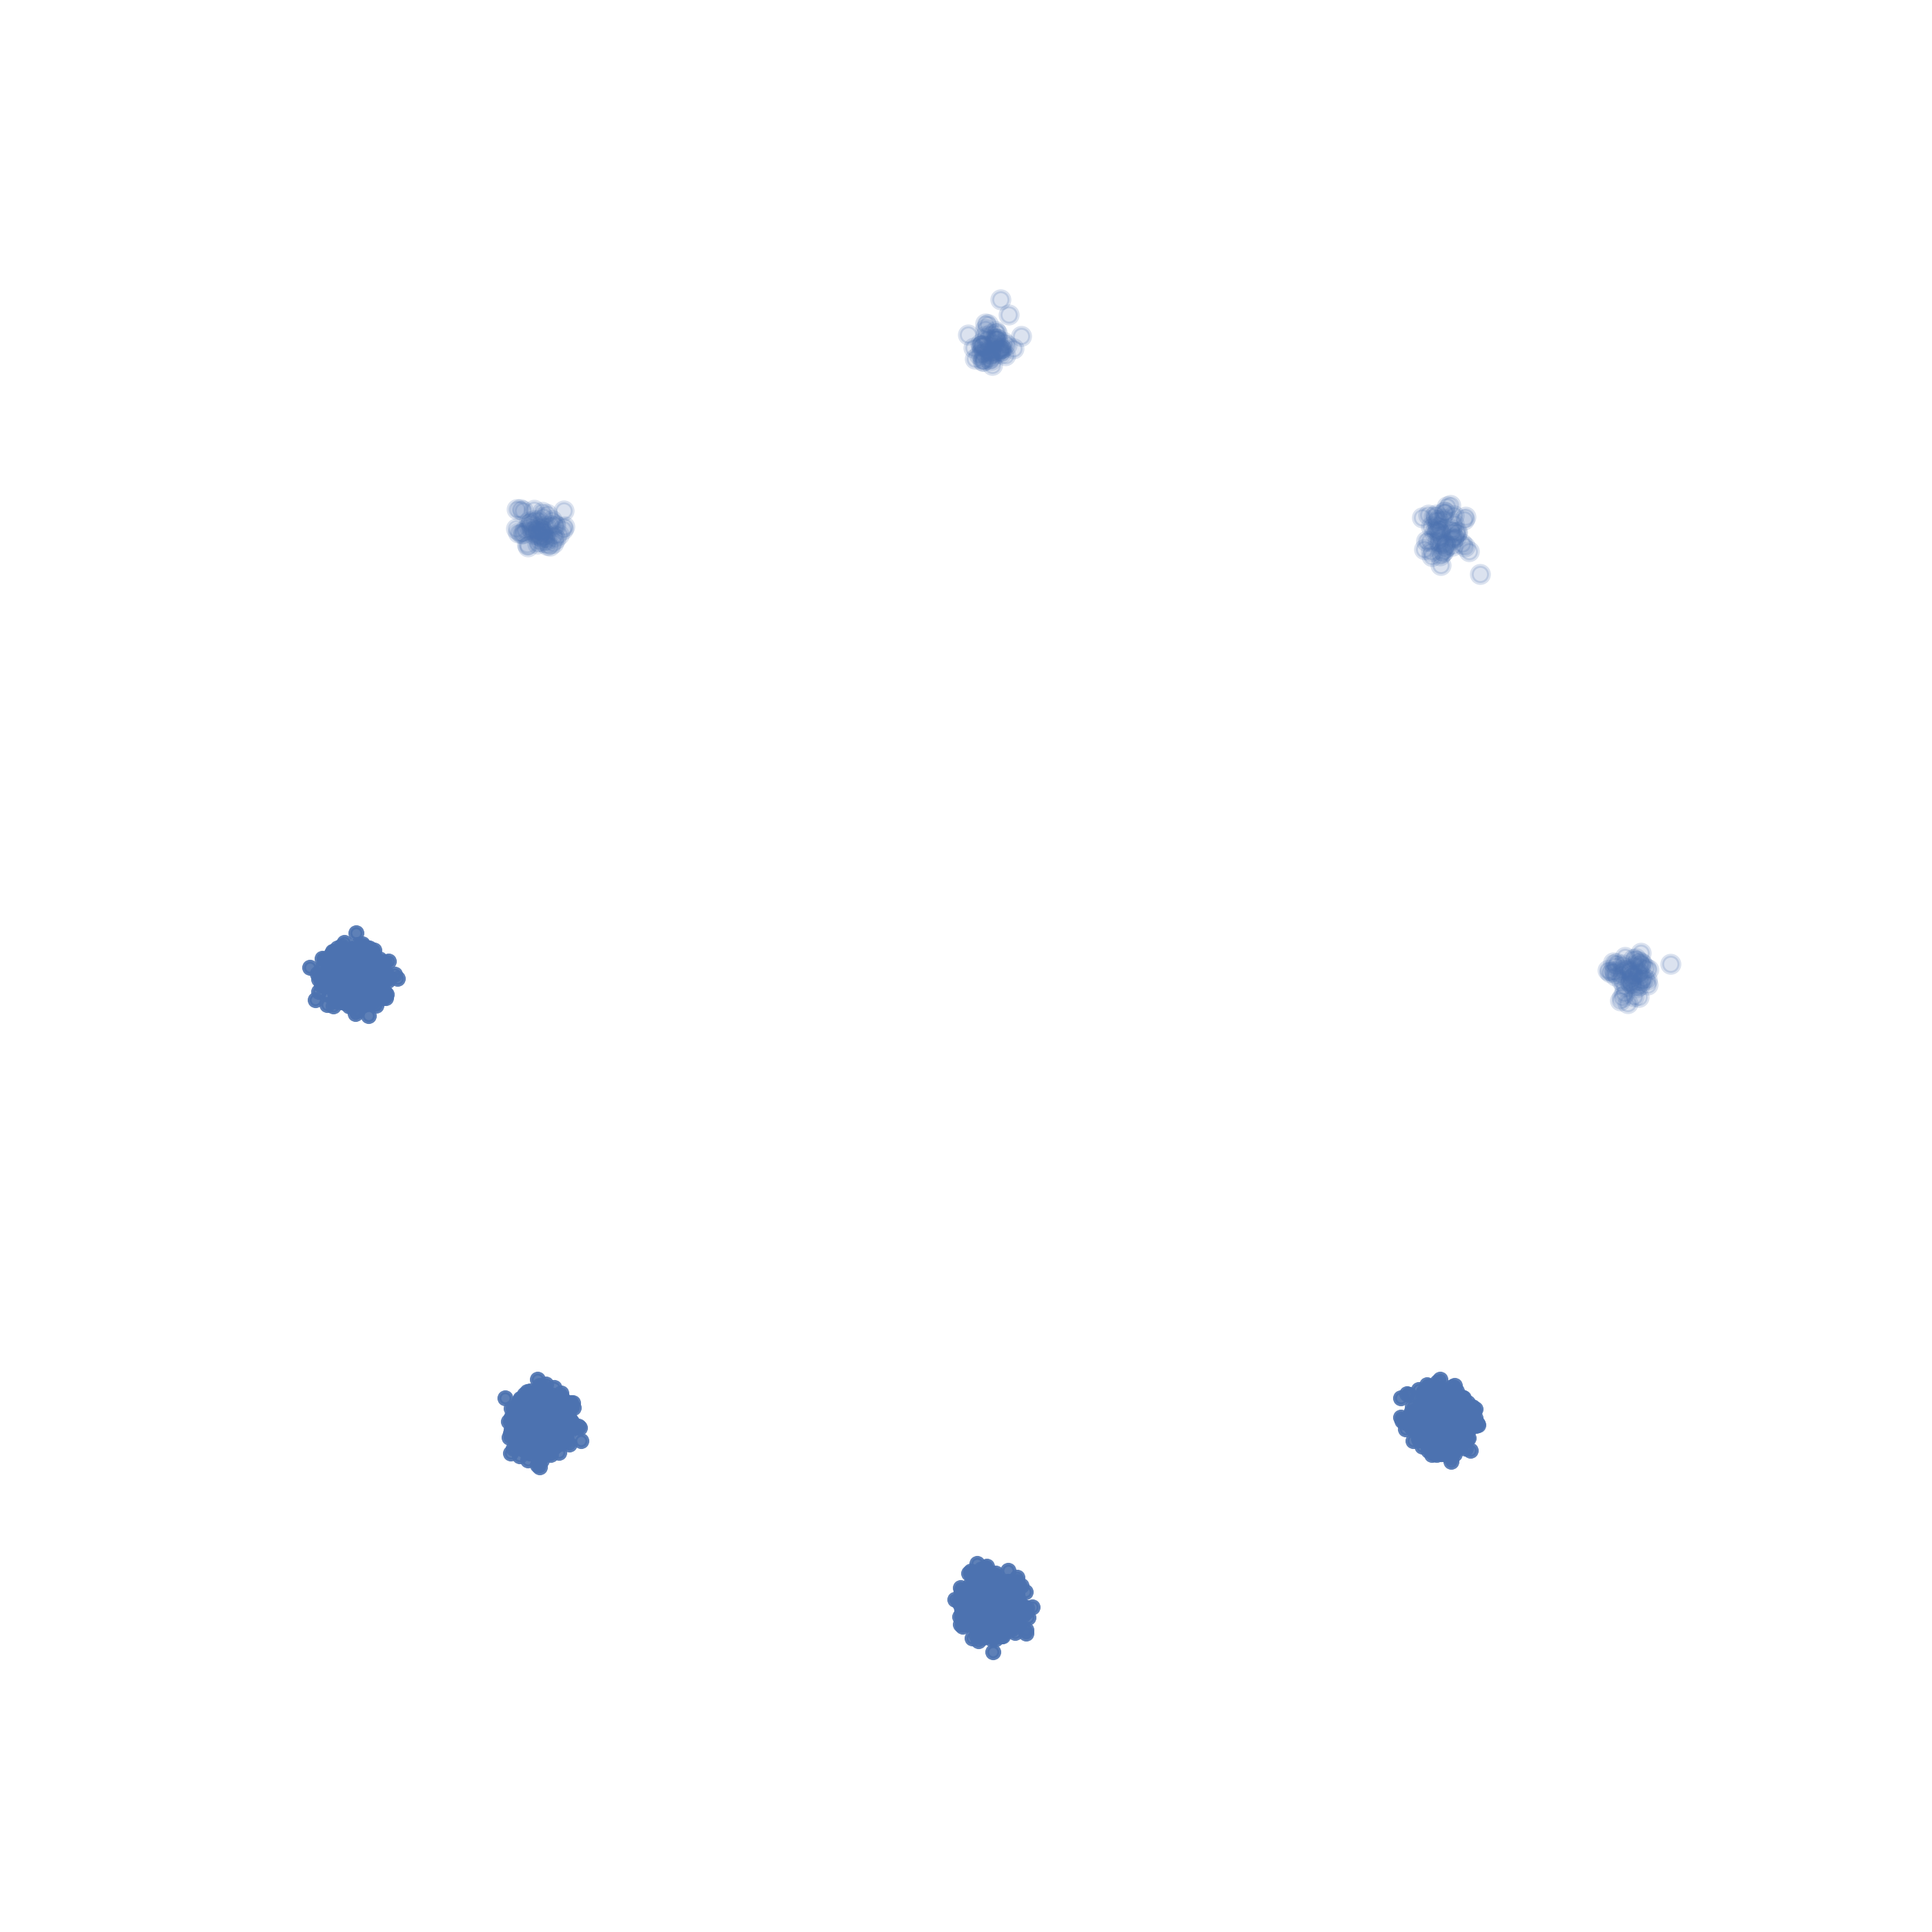
\includegraphics[width=0.8\textwidth]{Figures/Methods/ring_dataset.png}
    \end{subfigure}
    \hfill
    \begin{subfigure}{0.45\textwidth}
        \centering
        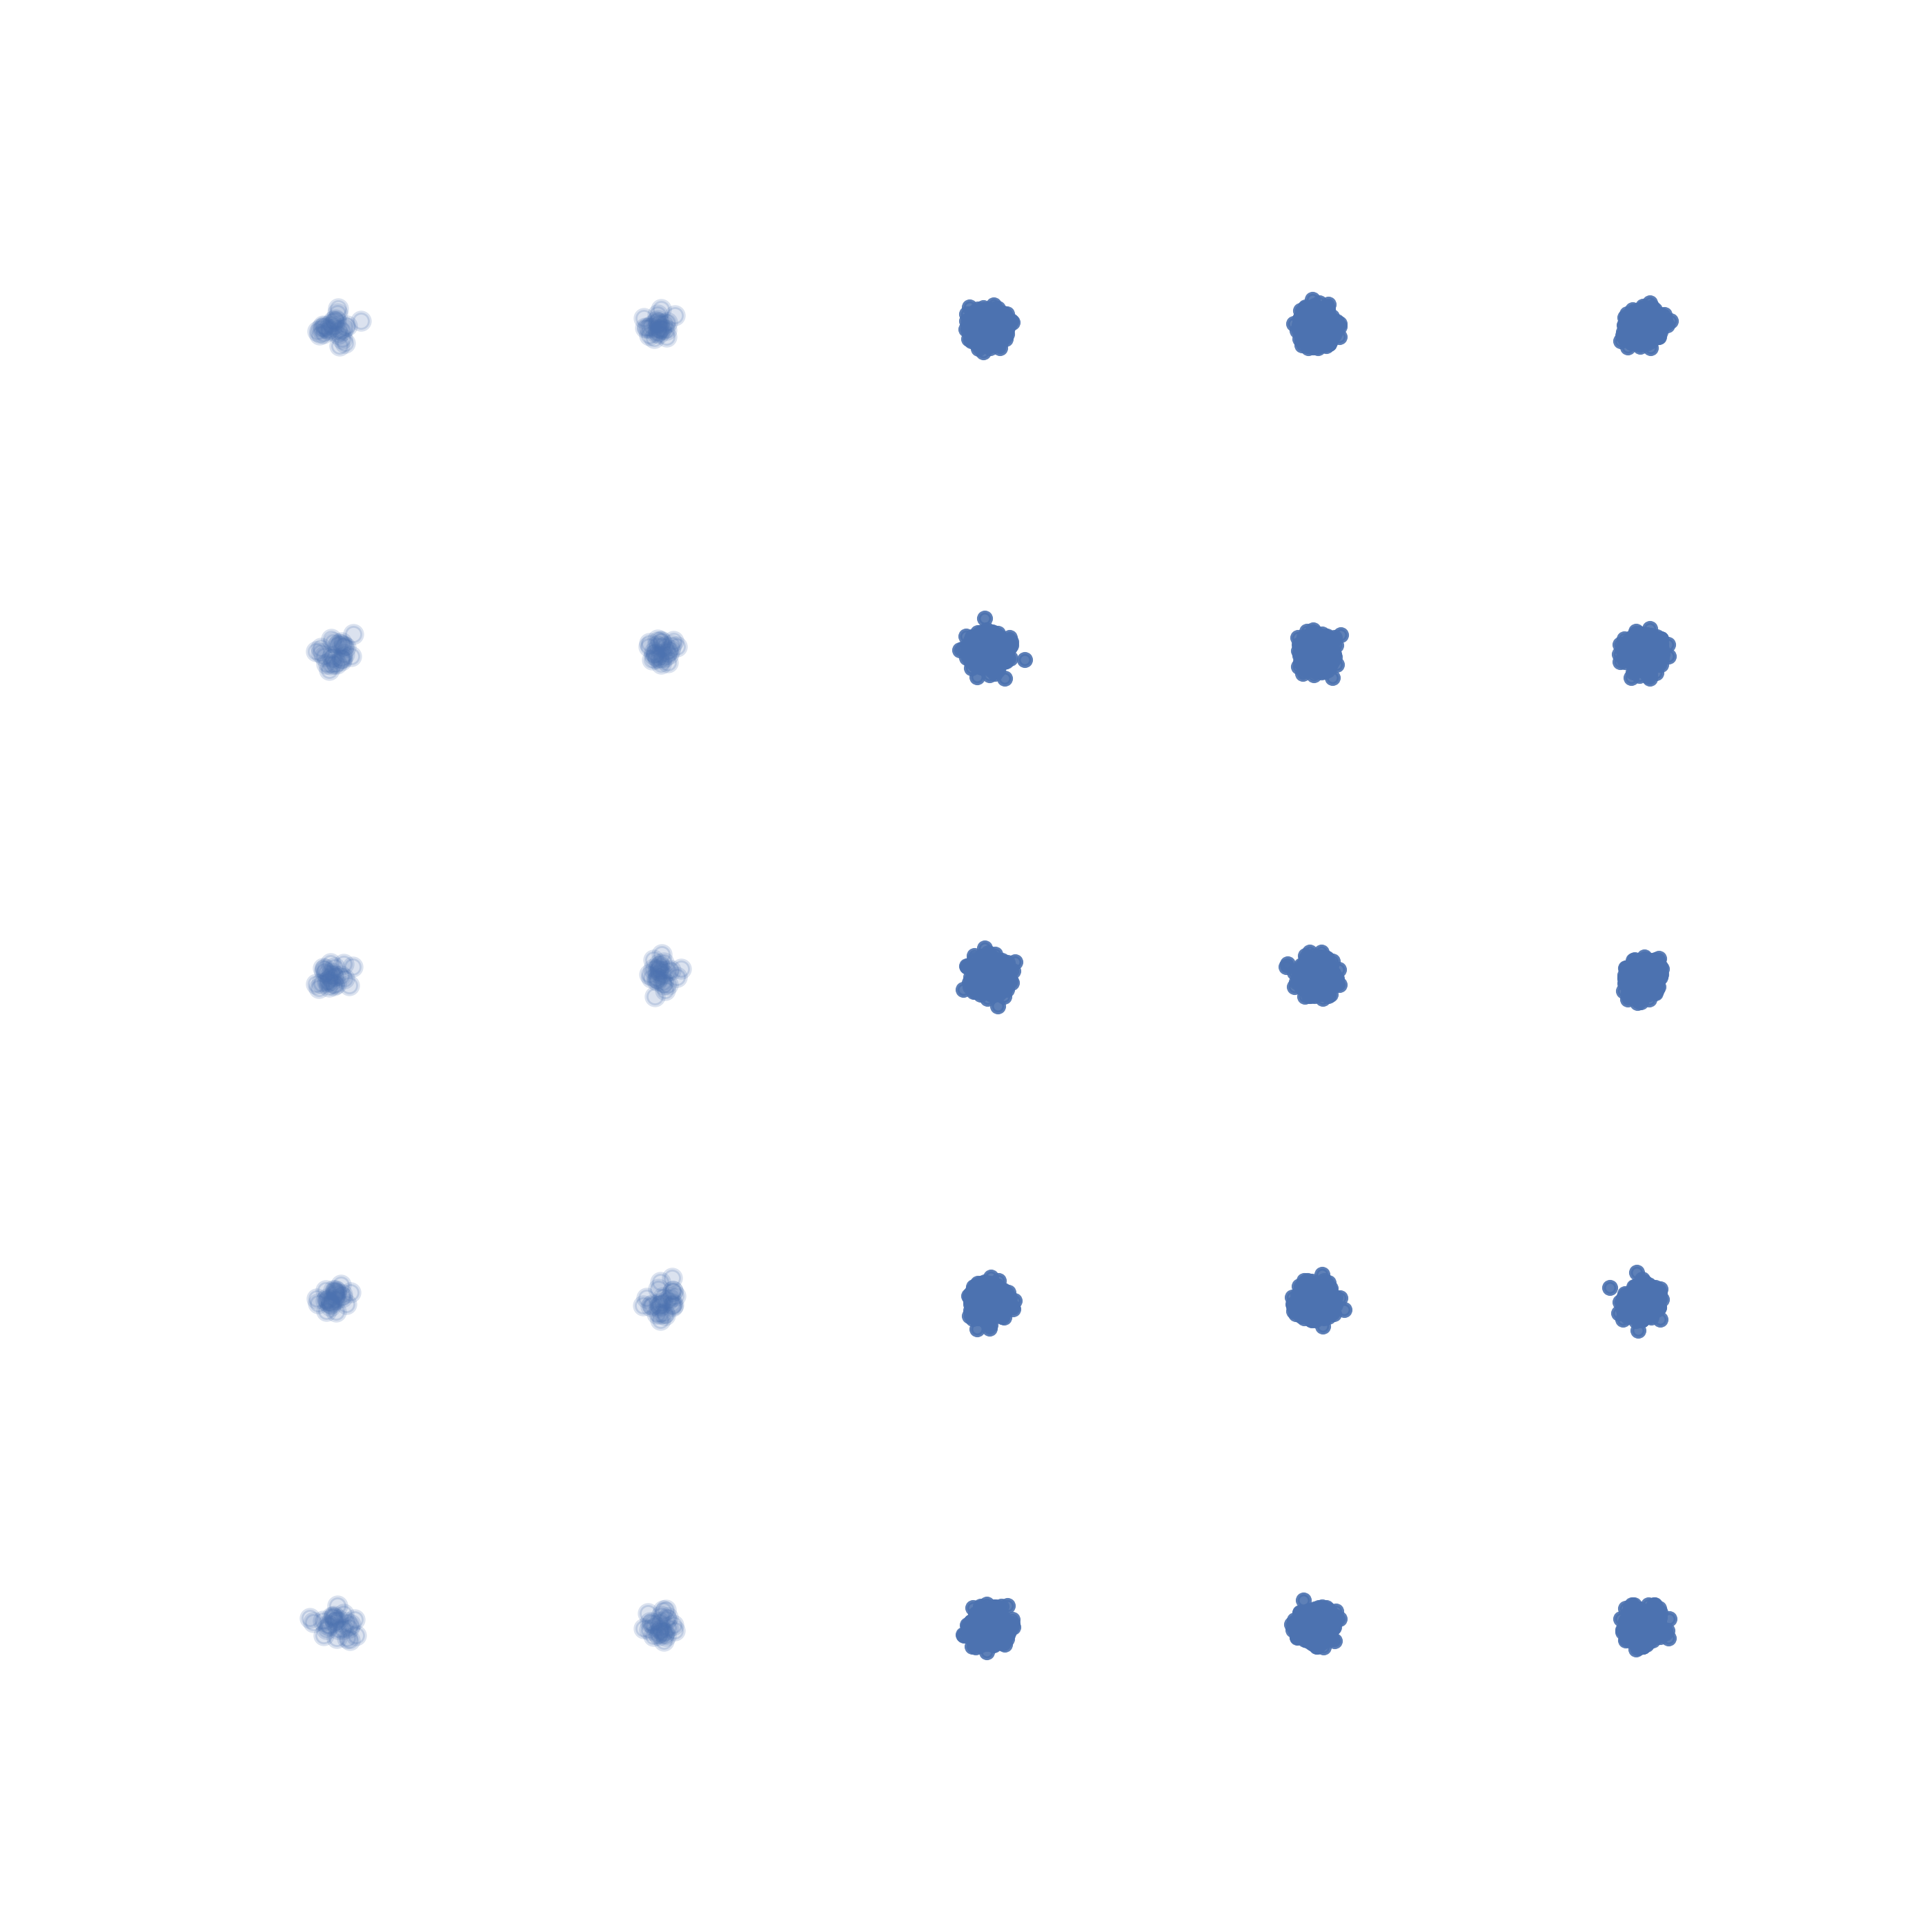
\includegraphics[width=0.8\textwidth]{Figures/Methods/grid_dataset.png}
    \end{subfigure}
    \caption{2D synthetic data: Ring(left) and Grid(right)}
    \label{fig-2d}
\end{figure}

    \item[Unbalanced 012-MNIST/MNIST dataset] For the natural dataset from the real world, we opt to employ MNIST as the first benchmark dataset for evaluating the effectiveness of different weighted sampling schemes. MNIST\cite{lecunGradientbasedLearningApplied1998} contains 60000 images of handwritten digits varying from 0 to 9, where the size of each image is fixed on $28\times 28$ with single color channel. We mainly consider two unbalanced variants of MNIST in our experiments. The first created dataset, namely unbalanced 012-MNIST, consists of only the digits 0, 1 and 2 where digit 2 is the minority class. Imbalance is artificially introduced by (randomly) reducing the number of digit 2 so that the probability of sampling digit 2 is smaller than that of sampling from other digits. The degree of depletion for digit 2 is determined by a specified imbalance ratio (i.e., ratio of the number of samples in minority class to the number of samples in majority class). The second dataset, unbalanced MNIST, consists of all the digits from 0 to 9. The digits 0, 1, 2, 3, and 4 have been selected as the minority classes, and their numbers are reduced as the same fashion in unbalanced 012-MNIST.  

    \item[Unbalanced Fashion MNIST dataset] Considering the relatively simple patterns of MNIST dataset, Fashion MNIST \cite{xiaoFashionMNISTNovelImage2017} is also used in our experiments for a more challenging replacement. Fashion MNIST consists of 60000 images of fashion items (e.g., different types of shoes and clothes) with 10 categories. Likewise in the MNIST setup, all images in Fashion MNIST are gray-scale with size $28\times 28$. Fashion MNIST is generally more complex due to the high variability in shapes and patterns among the images of different real fashion items. The same procedure in the MNIST case is leveraged to create the unbalanced version of Fashion MNIST dataset. Clothing and bag-related categories (T-shirt, Trouser, Pullover, Dress, Coat, Shirt, Bag) are set to minority classes while shoe-related categories (Sandal, Sneaker, Ankle boot) are considered as the majority classes. 
\end{description}


% For experiments on MNIST datasets, two unbalanced datasets out of MNIST are created. The first created dataset, unbalanced 012-MNIST, consists of only the digits 0, 1 and 2. The digit 2 is chosen as the minor class so that the probability of sampling 2 is smaller ($0.05p$, $0.10p$ and $0.30p$, $p$ is the sampling probability of majority classes) than that of sampling from the digit 0 or 1. The second dataset, unbalanced MNIST, consists of all the digits from 0 to 9. The digits 0, 1, 2, 3, and 4 have been selected as the minority classes, and their sampling probabilities are consistent with the minority class, digit 2, in the unbalanced 012-MNIST dataset.  


\subsection{Evaluation process \& metrics}
As for the evaluation part, 10k samples are randomly generated by each trained model. For the 2D synthetic datasets, valid samples are defined within 3 standard deviations of the nearest modes. A mode is covered by a certain model if there are at least 50 valid generated samples within 3 standard deviations of the mode's center. For image-based datasets, a well-trained classification model is employed to identify the labels of generated samples. Since our objective is to assess both the diversity and quality of the generated samples by different models, the following evaluation metrics are leveraged in our experiment.
\begin{description}[leftmargin=0pt]
    \item[Number of generated samples per mode] We measure mode coverage by counting the number of generated samples under each mode based on the prediction from a trained classifier. Ideally, the distribution of samples per mode should be close to a uniform distribution, which indicates each mode is well captured even though unbalanced training data is given. 

    \item[KL score] A follow-up metric, namely KL score, can be calculated based on the predicted labels of generated samples. KL score is obtained by computing the Kullback–Leibler (KL) divergence between the distribution of the classified labels from the generated samples with a balanced label distribution. We consider KL score as the primary metric to quantify the deviation of the label distribution of the generated samples from a uniform distribution. In the best case, KL score should be very close to zero indicating a balanced generation is acquired. This metric is widely used in various works related to addressing mode collapse problem in GANs \cite{schreursLeverageScoreSampling2022, anaissiDamageGANGenerative2024, yuInclusiveGANImproving2020, demeulemeesterBuresMetricGenerative2021}.

    \item [FID] So far, the above two metrics are both label-based, which means they merely measure the imbalance under the class level. However, the imbalance could occur in both inter-class and intra-class. Additionally, a well-balanced generation does not necessarily ensure results with high quality. For example, the patterns of the generated samples could be highly diverse, but the overall generation could be considered poor quality due to blurriness, weird distortions, and incorrect proportions. Therefore, we propose to employ Fr\'{e}chet Inception Distance (FID) \cite{heuselGANsTrainedTwo2017} as a supplementary evaluation tool for assessing both the diversity and quality of generated images. The nature of FID is to measure the similarity between the distributions of real data and generated data. To compute FID, a pre-trained classifier (normally we use inception-V3) is implemented to extract features of image data, FID is then given by the Fr\'{e}chet distance of two Gaussian distributions: 
    \begin{equation}
        \text{FID} = \| \bmu_r - \bmu_g \|^2 + \text{Tr}(\bSigma_r + \bSigma_g - 2(\bSigma_r \bSigma_g)^{1/2})
    \end{equation}
    where $\bmu_r,\bmu_g$ are the means and $\bSigma_r,\bSigma_g$ are the covariance matrices of extracted embedding of real and generated images, respectively. The reference statistics (i.e., $\bmu_r, \bSigma_r$) are computed based on the (class) balanced dataset in all experiments. A low FID score implies that the distribution of generated images closely matches the distribution of balanced training samples, indicating a more diverse and higher-quality generation.
    
\end{description}


% In the model evaluation part, 10k samples are generated by each trained model. For MNIST-related generation, a pre-trained classification model (resnet18 trained up to 99.43\% accuracy) is used to classify the generations. Since our objective is to improve the diversity of the generated samples under unbalanced input conditions, besides descriptive statistics, KL divergence (Kullback–Leibler divergence) is used as the primary metric to measure the deviation of the distribution of the generated samples from a uniform distribution. And FID (Frechet Inception Distance score) is used to measure the quality of the generated samples (for MNIST-related and Fashion MNIST datasets). For the 2D synthetic datasets, valid samples are defined within 3 standard deviations of the nearest modes. A mode is covered by a certain model if there are at least 50 valid generated samples within 3 standard deviations of the mode's center. 

\subsection{Hyperparameter details}
\label{subsec-setup-hyperparameter}
In this section, we outline the key hyperparameters used in the experiment part. Unless otherwise specified, the hyperparameter settings used in the subsequent experiment part will default to those mentioned below.
\begin{description}[leftmargin=0pt]
    \item[Hyperparameters for Gen-RKM ] The basic hyperparameter settings for training Gen-RKM is displayed in Table \ref{tab-Gen-RKM-setting}. We generally follow the same configurations as those in \cite{pandeyGenerativeRestrictedKernel2021}, except that we slightly increase the dimension of the feature map and the mini-batch size. Considering our experiments required re-training the models multiple times, and the sizes of used datasets are relatively large. To maintain more computationally efficient training, Gen-RKM is computed in the primal form across all our experiments (i.e., eigen-decomposition on the covariance matrix), which necessitates $d_f < m$ to guarantee that the covariance matrix is full rank for more stable computations \cite{pandeyGenerativeRestrictedKernel2021}.
    \begin{table}[ht]
\centering
\begin{tabular}{>{\raggedright\arraybackslash}m{8cm} >{\centering\arraybackslash}m{2cm} >{\centering\arraybackslash}m{2cm} >{\centering\arraybackslash}m{2cm}}
\toprule
\multirow{2}{*}{Hyperparameter} & \multicolumn{3}{c}{Dataset} \\
\cmidrule(lr){2-4}
 & 2D Ring/Grid & 012-MNIST  & MNIST/Fashion \\
\midrule
regularization parameters: $\{\eta,c_{\text{stab}},\gamma_{\text{RKM}}\}$ & \{1;1;100\} & \{1;1;100\}  & \{1;1;100\}  \\
dimension of feature map: $d_f$ & 128 & 300 &300 \\
dimension of latent space: $s$ & 8/25 & 10 & 10 \\
mini-batch size: $m$ & 256 & 328 & 328 \\
maximum epoch number: $N_{\text{epoch}}$ & 150 & 100 & 150\\
number of Gaussian components in GMM: $l$ &8/25 & 3 & 10 \\
learning rate & 0.0001 & 0.0001 & 0.0001 \\
\bottomrule
\end{tabular}
\caption{Hyperparameter settings for Gen-RKM}
\label{tab-Gen-RKM-setting}
\end{table}


    \item[Neural network architectures] The detailed neural network architectures for the feature map and the pre-image map in Gen-RKM are summarized in Table \ref{tab-network-architecture}. For 2D synthetic data, the architecture includes 3 fully connected layers with ReLU activation functions in between. For MNIST-related datasets, the architecture consists of 2 convolutional layers, and ReLU activations are implemented similarly.
    \begin{table}[ht]
\centering
\begin{tabular}{lccc}
\toprule
\multirow{2}{*}{Dataset} & \multirow{2}{*}{Input size} & \multicolumn{2}{c}{Architecture} \\
\cmidrule(lr){3-4}
 & & Feature map & Pre-image map \\
\midrule
2D Ring/Grid & $2$ & \makecell{FC 32 (Linear)\\ ReLu($\alpha=0.2$) \\ FC 64 (Linear) \\ ReLu($\alpha=0.2$) \\ FC 128 (Linear) } &  reverse of fm \\
\midrule
012-MNIST/MNIST/Fashion& $28\times 28\times 1$ & \makecell{Conv $32\times 4\times 4$\\ReLu($\alpha=0.2$) \\ Conv $64\times 4\times 4$ \\ ReLu($\alpha=0.2$) \\ FC 300 (Linear)}   & reverse of fm   \\


\bottomrule
\end{tabular}
\caption{Details of network architectures used in Gen-RKM. All convolutional layers and transposed convolutional layers have stride 2 and padding 1. Pre-image map is the reverse of feature map architecture, except that a sigmoid activation function is implemented for the output layer \cite{pandeyGenerativeRestrictedKernel2021}.}
\label{tab-network-architecture}
\end{table}


    \item[Hyperparameters for RLS sampling] Regarding the hyperparameters used in RLS sampling, we generally adopt the same settings as in the original work of RLS-GAN \cite{schreursLeverageScoreSampling2022}. More specifically, the ridge regularization parameter is set to 0.0001, and feature maps in kernel ridge regression are reduced to $k=25$ by either UMAP or Gaussian sketching. However, Instead of using Inception-v3 as mentioned in \cite{schreursLeverageScoreSampling2022}, we empirically observe that RLS sampling with an explicit feature map based on AlexNet could achieve better performance. Therefore, throughout the experiments, the pre-trained classifier-based RLS sampling is computed using the embeddings extracted from the next-to-the-last layer of Alexnet (which has already been pre-trained on the ImageNet dataset). One can refer to Section \ref{subsec-additional-studies} for the detailed results of the ablation study on the impact of different pre-trained classifiers on the performance of RLS sampling.

    \item[Hyperparameters for Iforest sampling] Fine-tuning the parameters in Isolation Forest is challenging and typically requires some labeled data for validation. However, since no prior information regarding labels is provided in a fully unsupervised manner,  we use the default hyperparameter settings provided in the \href{https://scikit-learn.org/stable/modules/generated/sklearn.ensemble.IsolationForest.html}{\texttt{sklearn}} package.
\end{description}



\section{Experiments on inverse frequency sampling under supervised setting}
\label{sec-expr-supervised}

\subsection{Unbalanced MNIST/Fashion MNIST}
Given that inverse frequency sampling transforms the input distribution into a uniform one, there’s a definite and notable improvement in the diversity of the generated samples. Figure \ref{dis-ub09} shows the distributions of the generated samples from Gen-RKM and Gen-RKM with inverse frequency sampling using MNIST and Fashion MNIST datasets respectively. The minority classes are shown in red and the normal classes are in blue. The improvement in generation diversity is notable. Figures \ref{fig-ub09} visualizes the random generation of Gen-RKM using the MNIST and FashionMNIST datasets, before and after applying inverse frequency sampling. In these figures, the minority classes are highlighted with red rectangles. 

\begin{figure}[H]
    \centering
    \begin{subfigure}{0.45\textwidth}
        \centering
        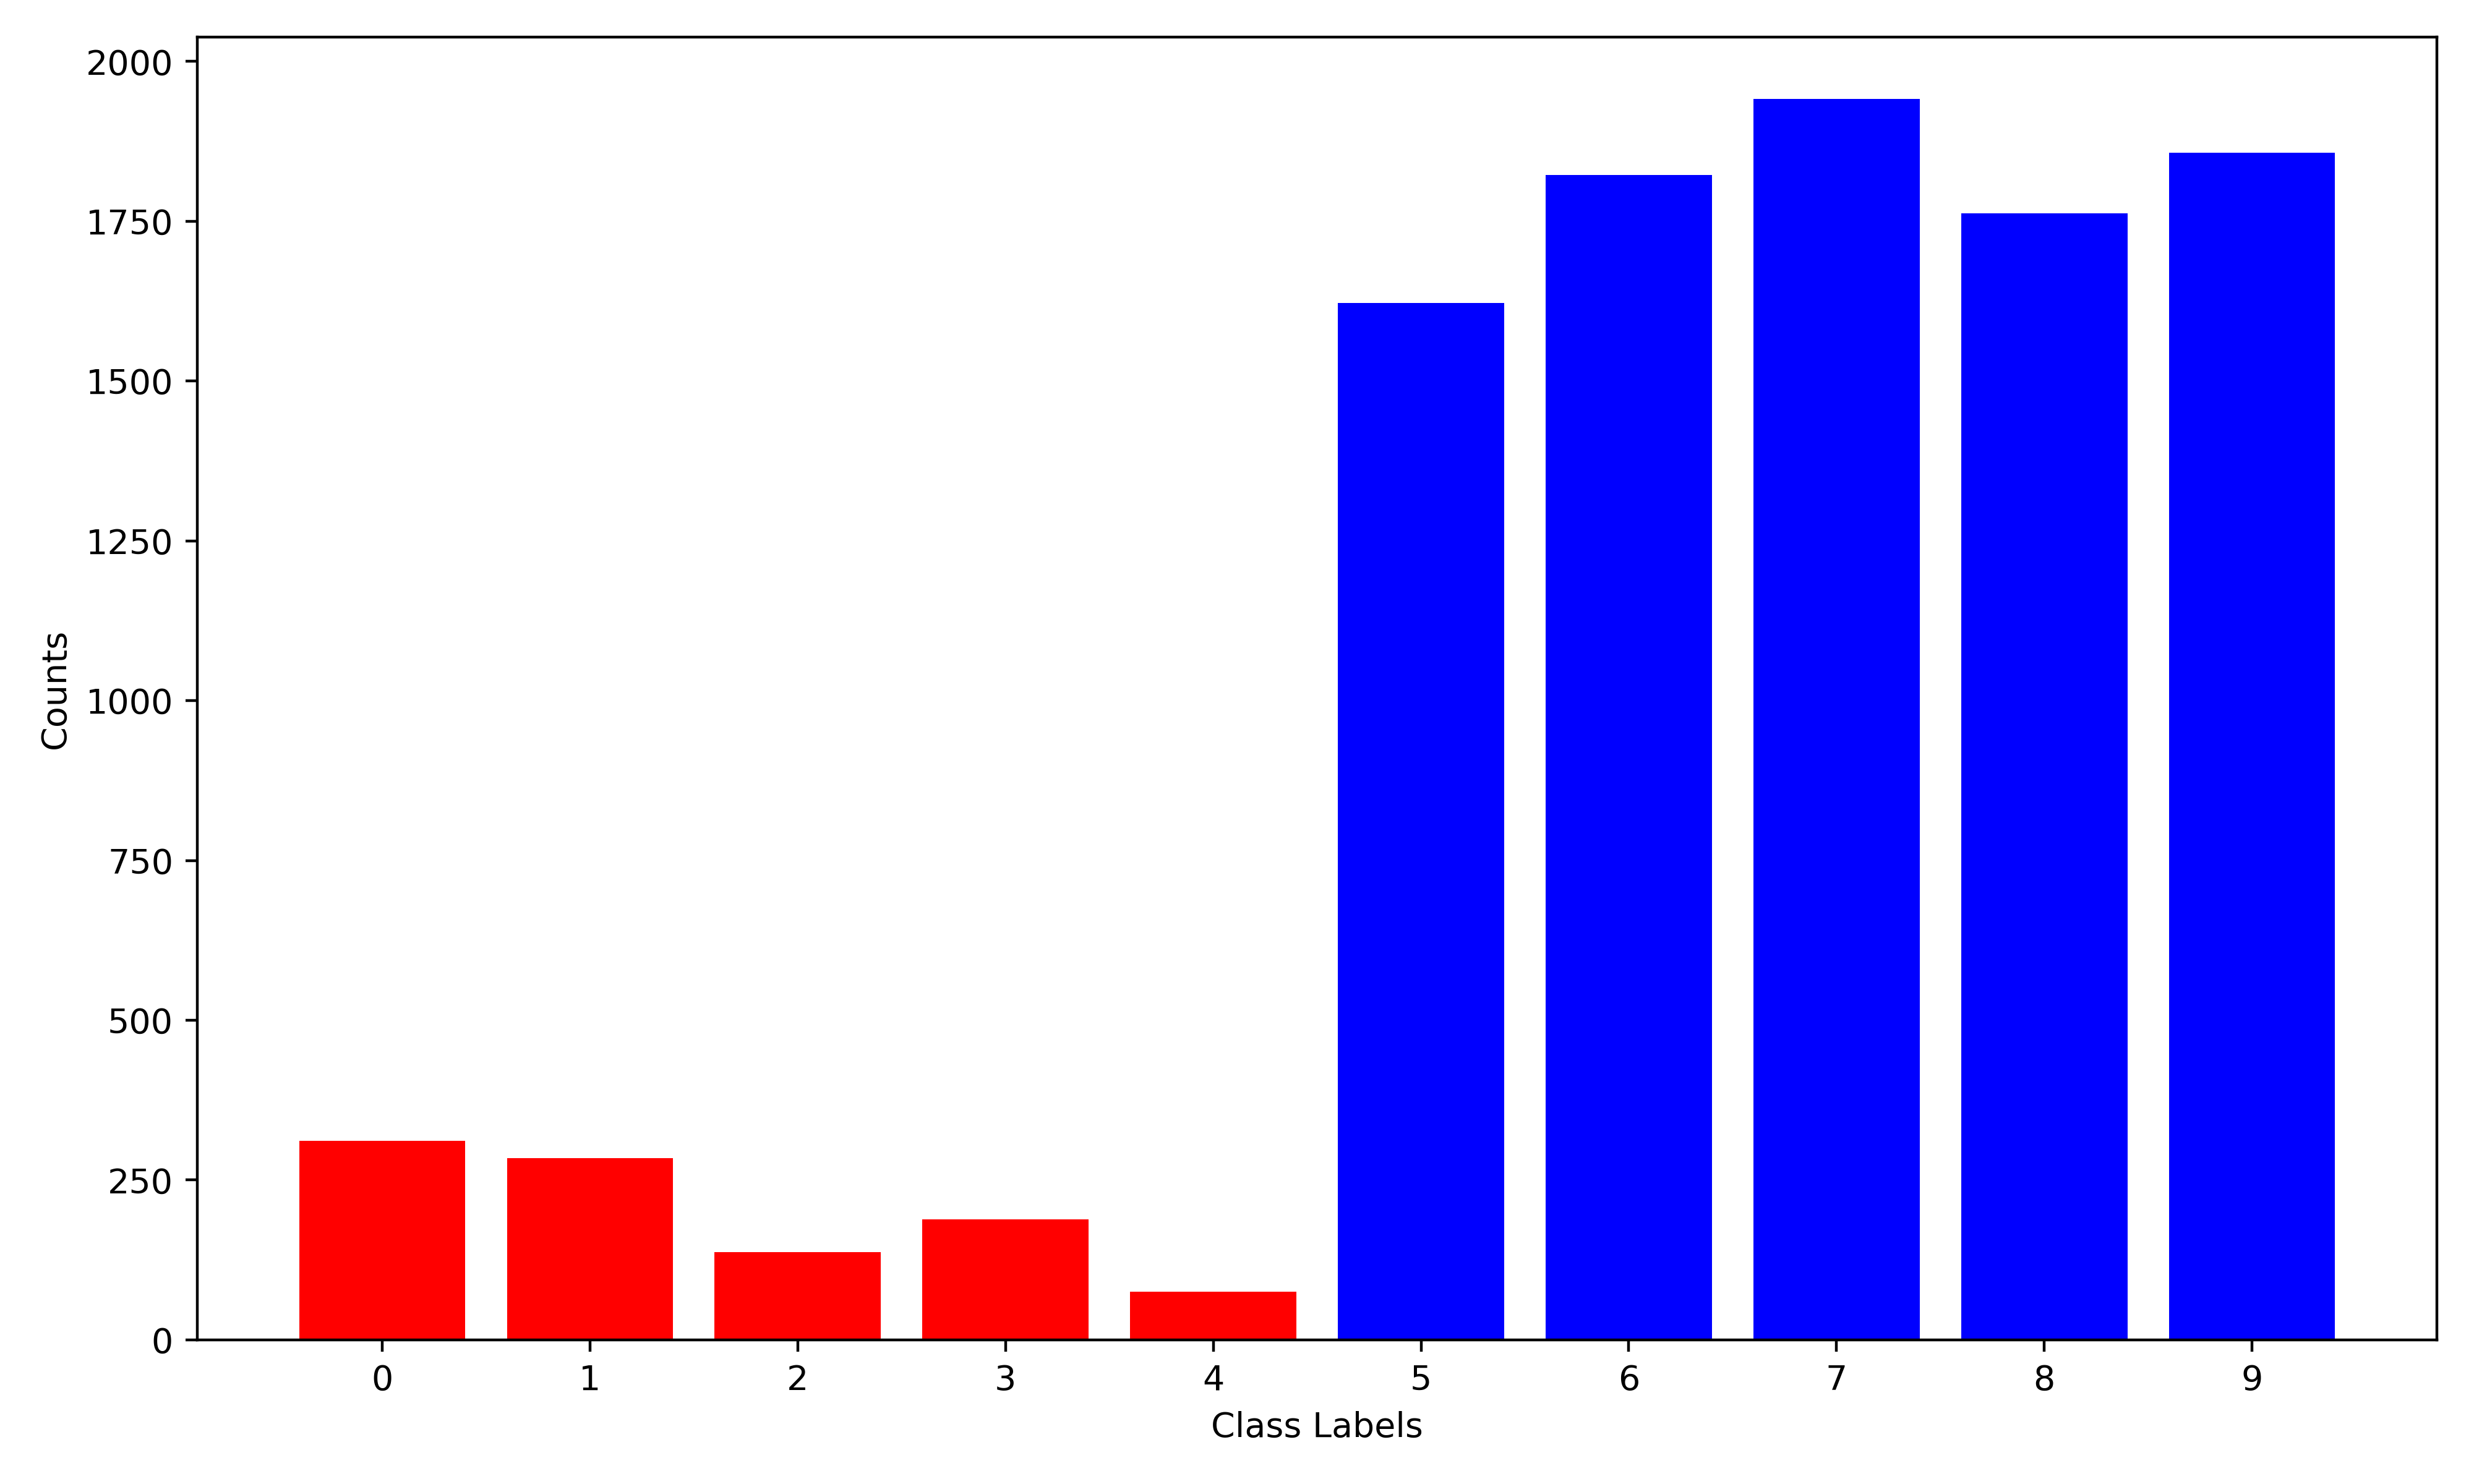
\includegraphics[width=0.8\textwidth]{Figures/Methods/dis_ub09.png}
    \end{subfigure}
    \hfill
    \begin{subfigure}{0.45\textwidth}
        \centering
        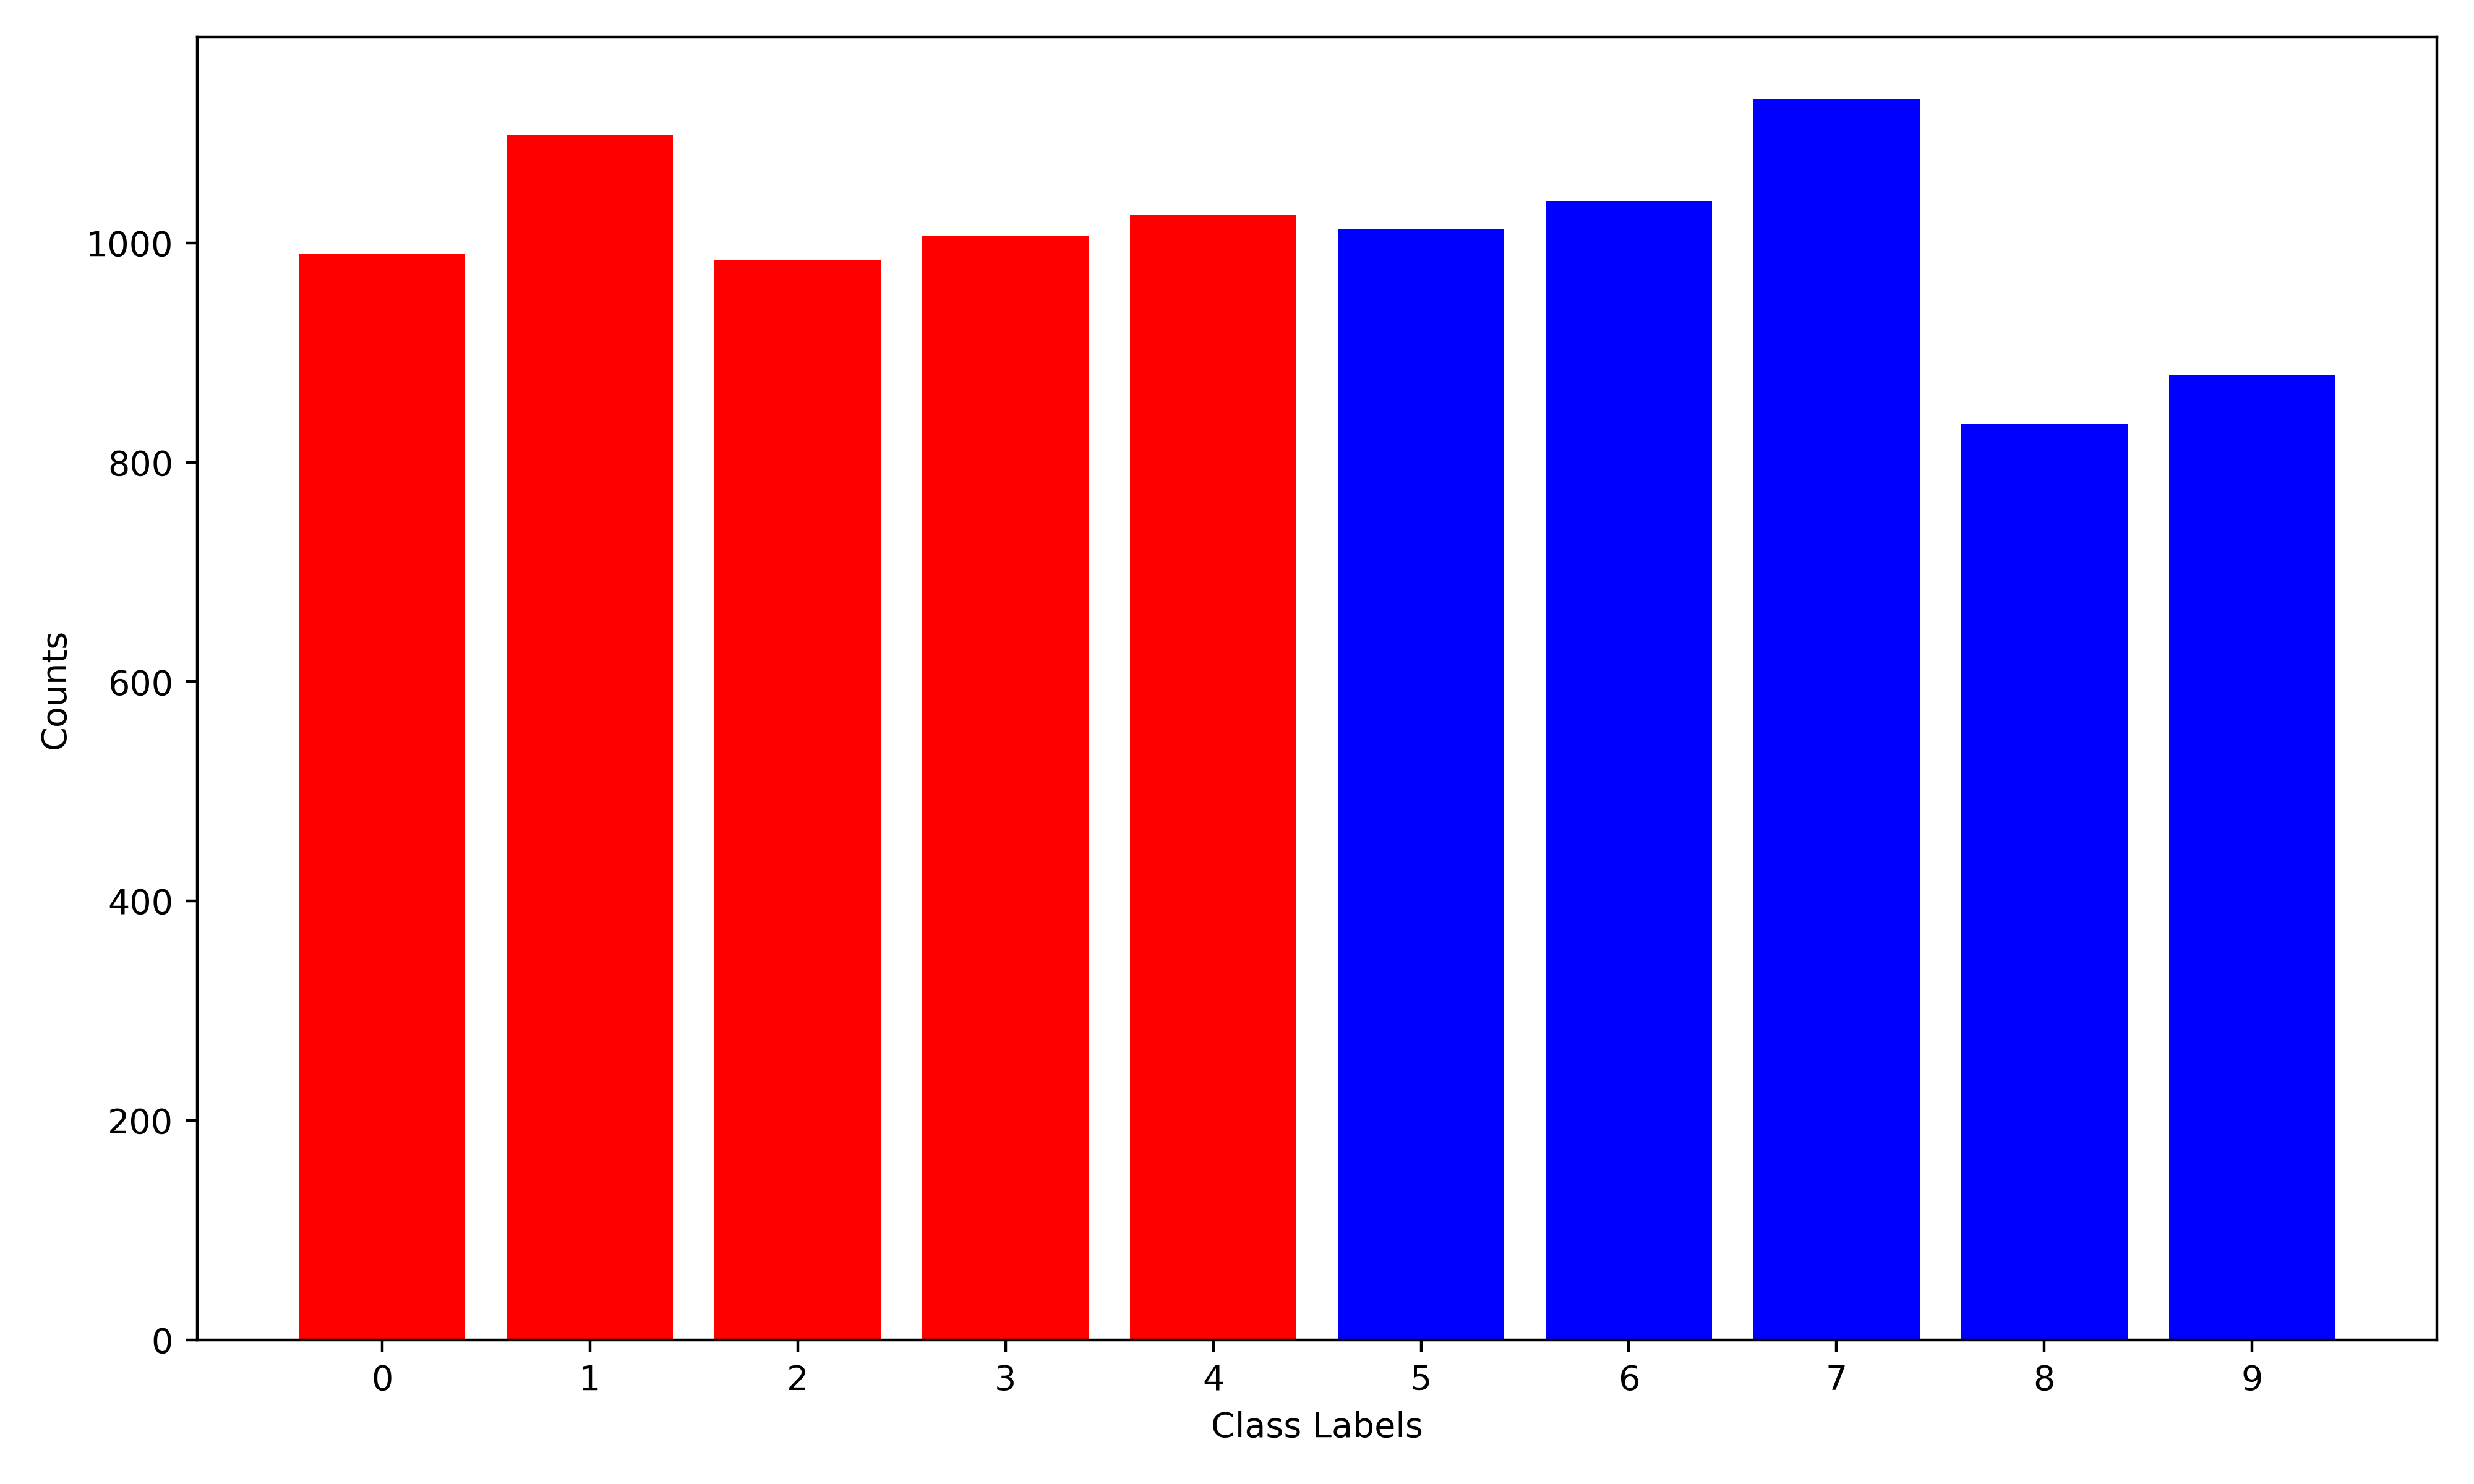
\includegraphics[width=0.8\textwidth]{Figures/Methods/dis_ub09_inw.png}
    \end{subfigure}
    \hfill
    \begin{subfigure}{0.45\textwidth}
        \centering
        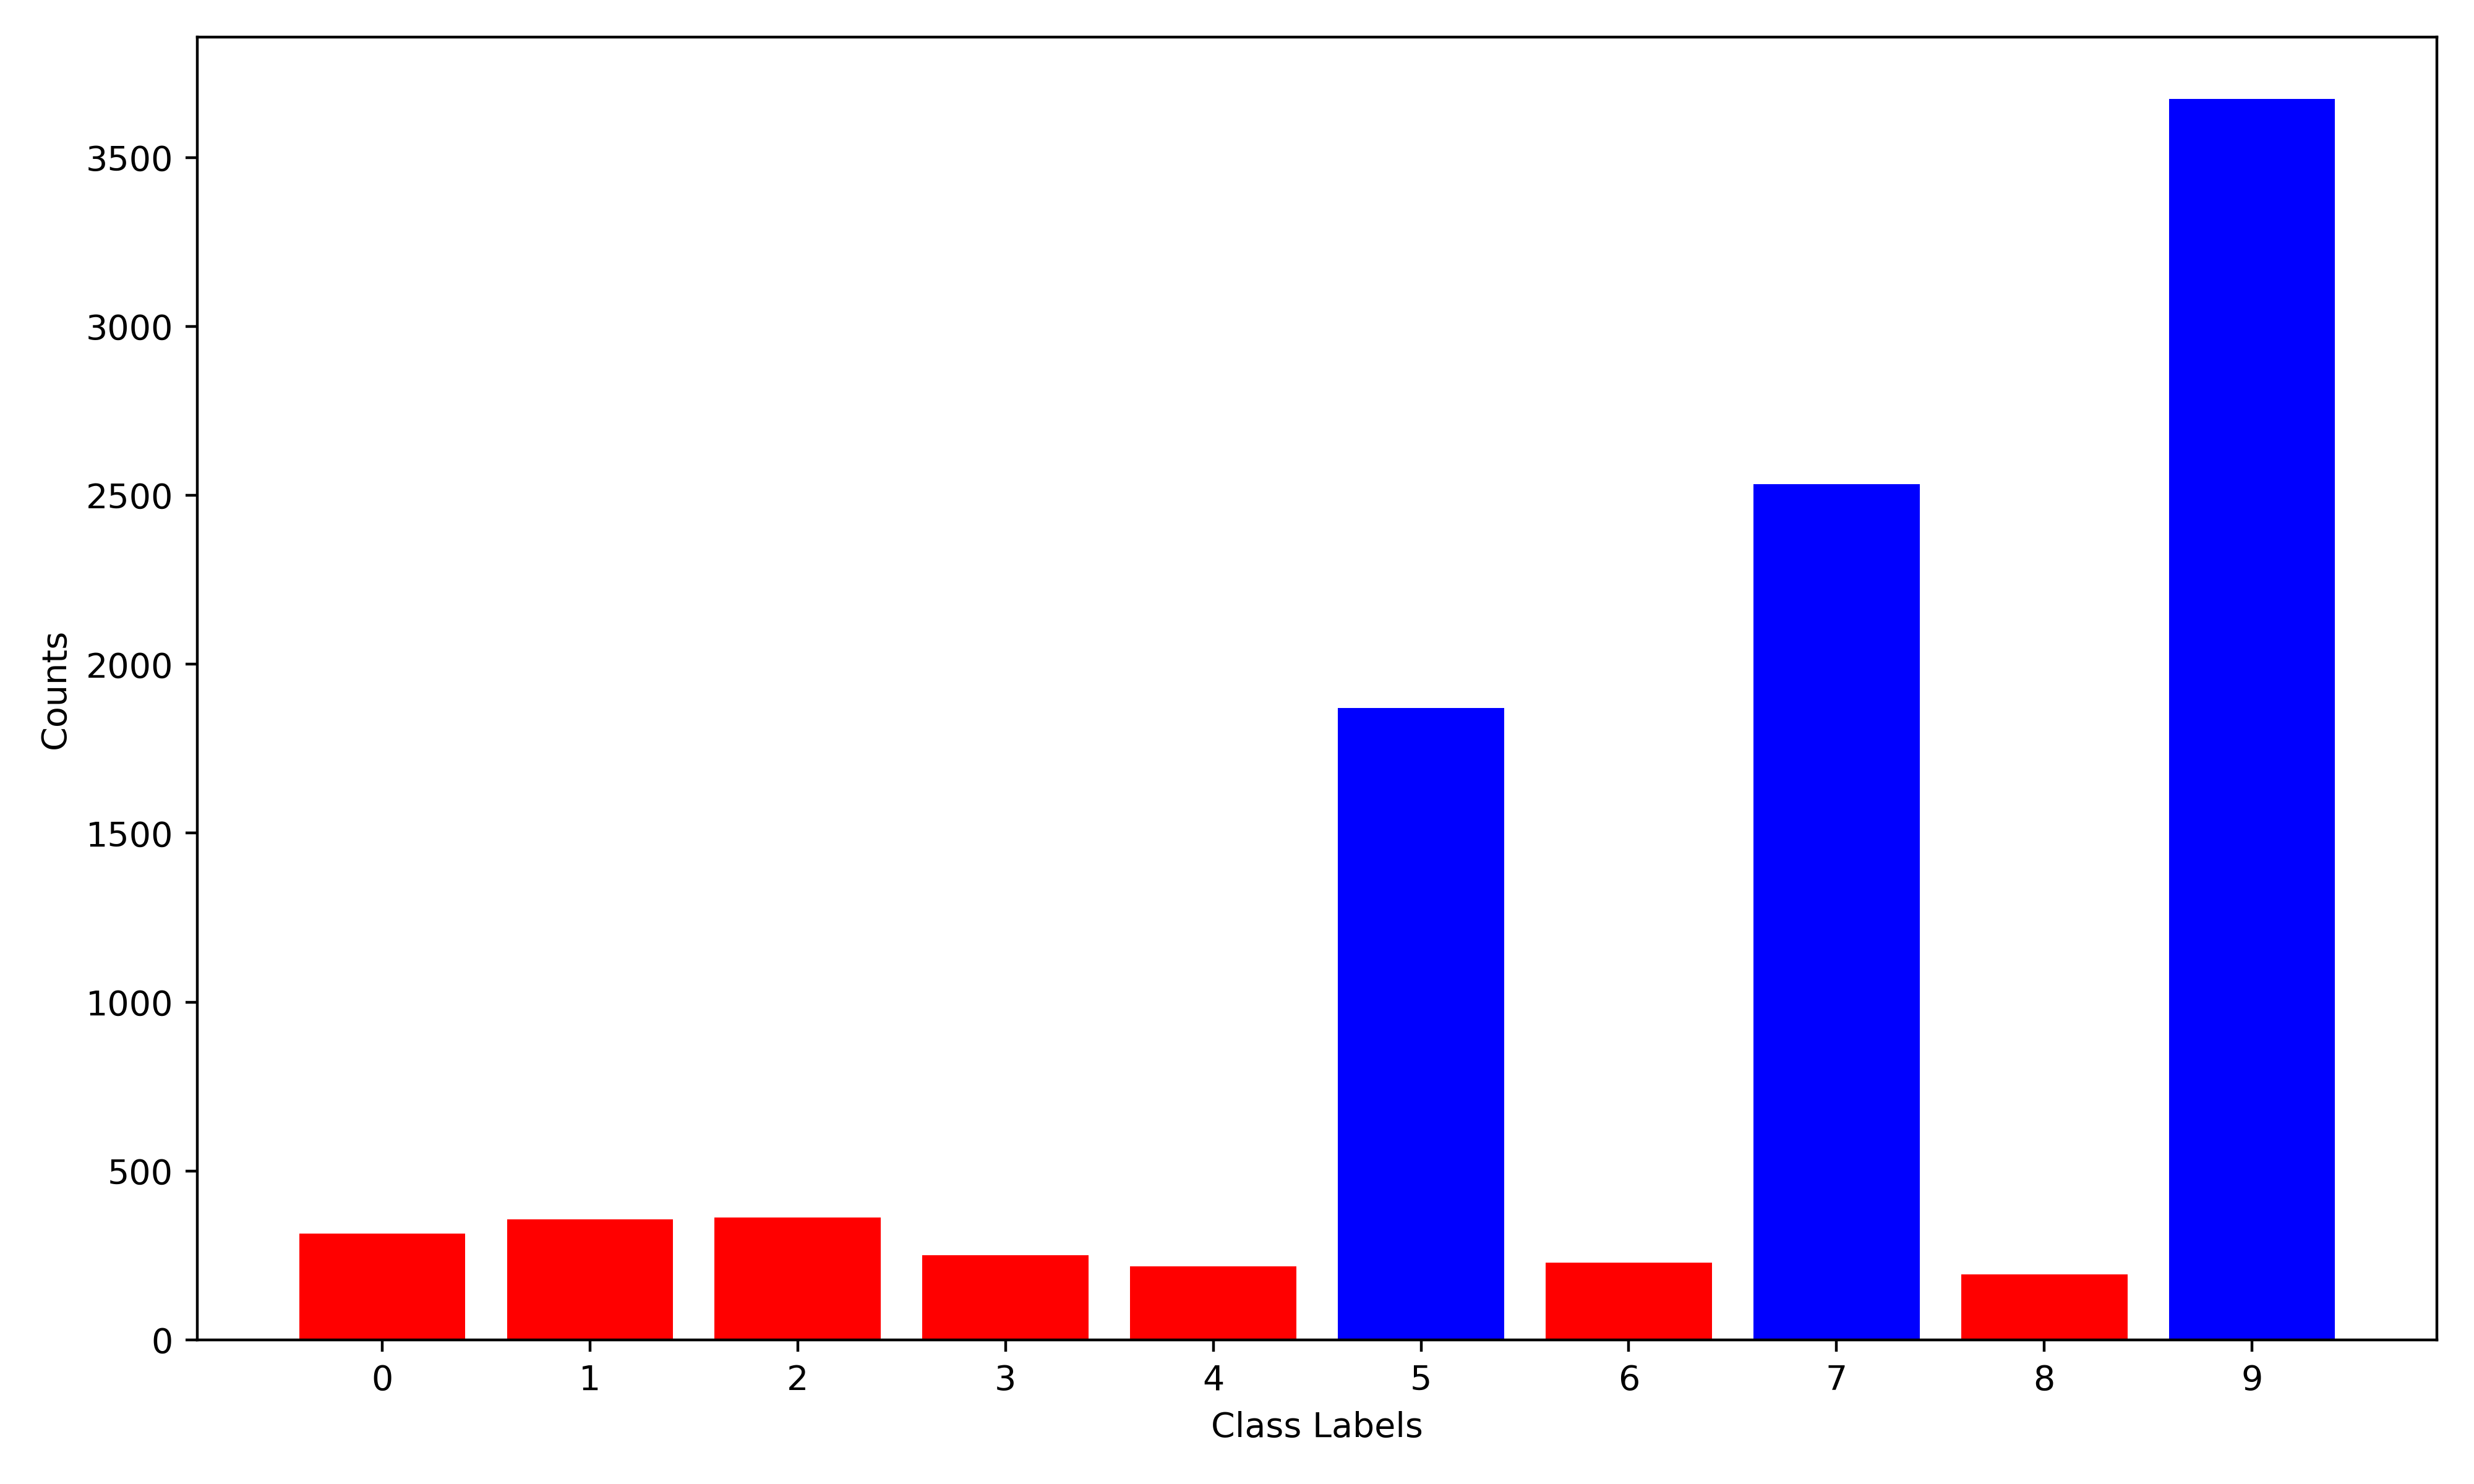
\includegraphics[width=0.8\textwidth]{Figures/Methods/dis_ubfs.png}
    \end{subfigure}
    \hfill
    \begin{subfigure}{0.45\textwidth}
        \centering
        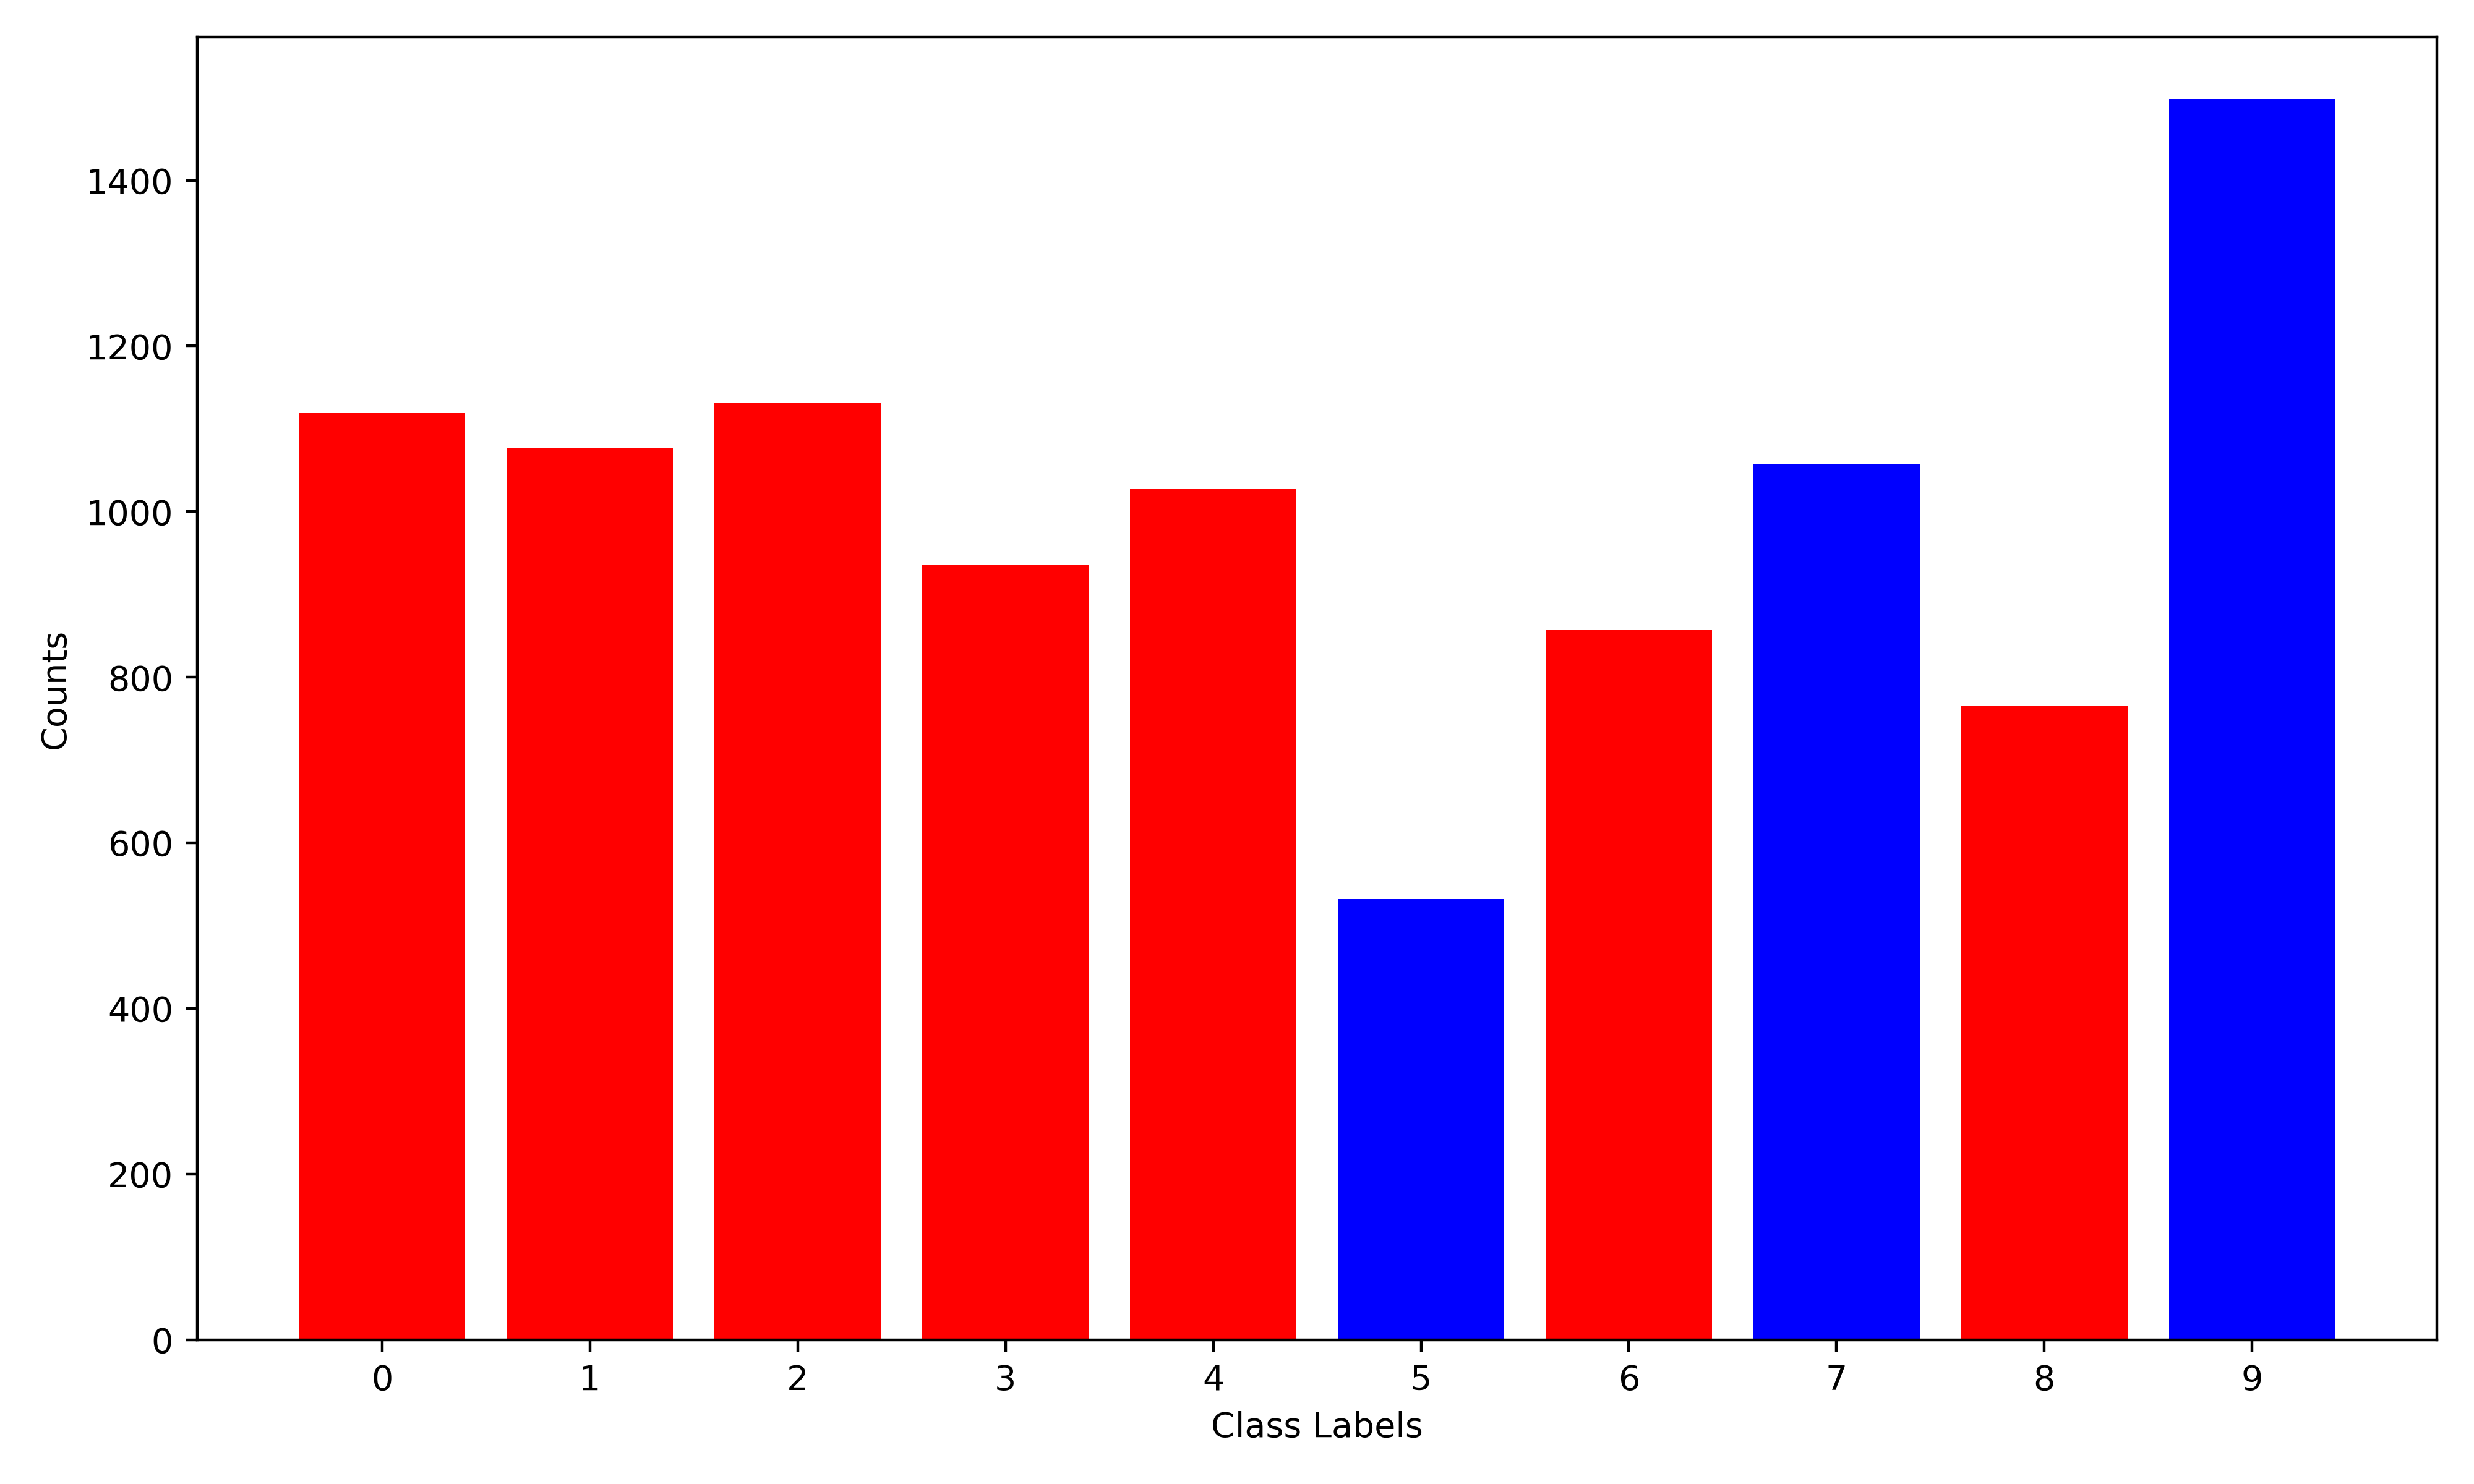
\includegraphics[width=0.8\textwidth]{Figures/Methods/dis_ubfs_inw.png}
    \end{subfigure}
    \caption{Number of generated samples in each class for the unbalanced MNIST dataset: Vanilla Gen-RKM (top left) vs. Gen-RKM with inverse frequency sampling (top right). For the Fashion MNIST dataset: Vanilla Gen-RKM (down left) vs. Gen-RKM with inverse frequency sampling (down right). A rebalancing effect is visible}
    \label{dis-ub09}
\end{figure}



\begin{figure}[H]
    \centering
    \begin{subfigure}{0.45\textwidth}
        \centering
        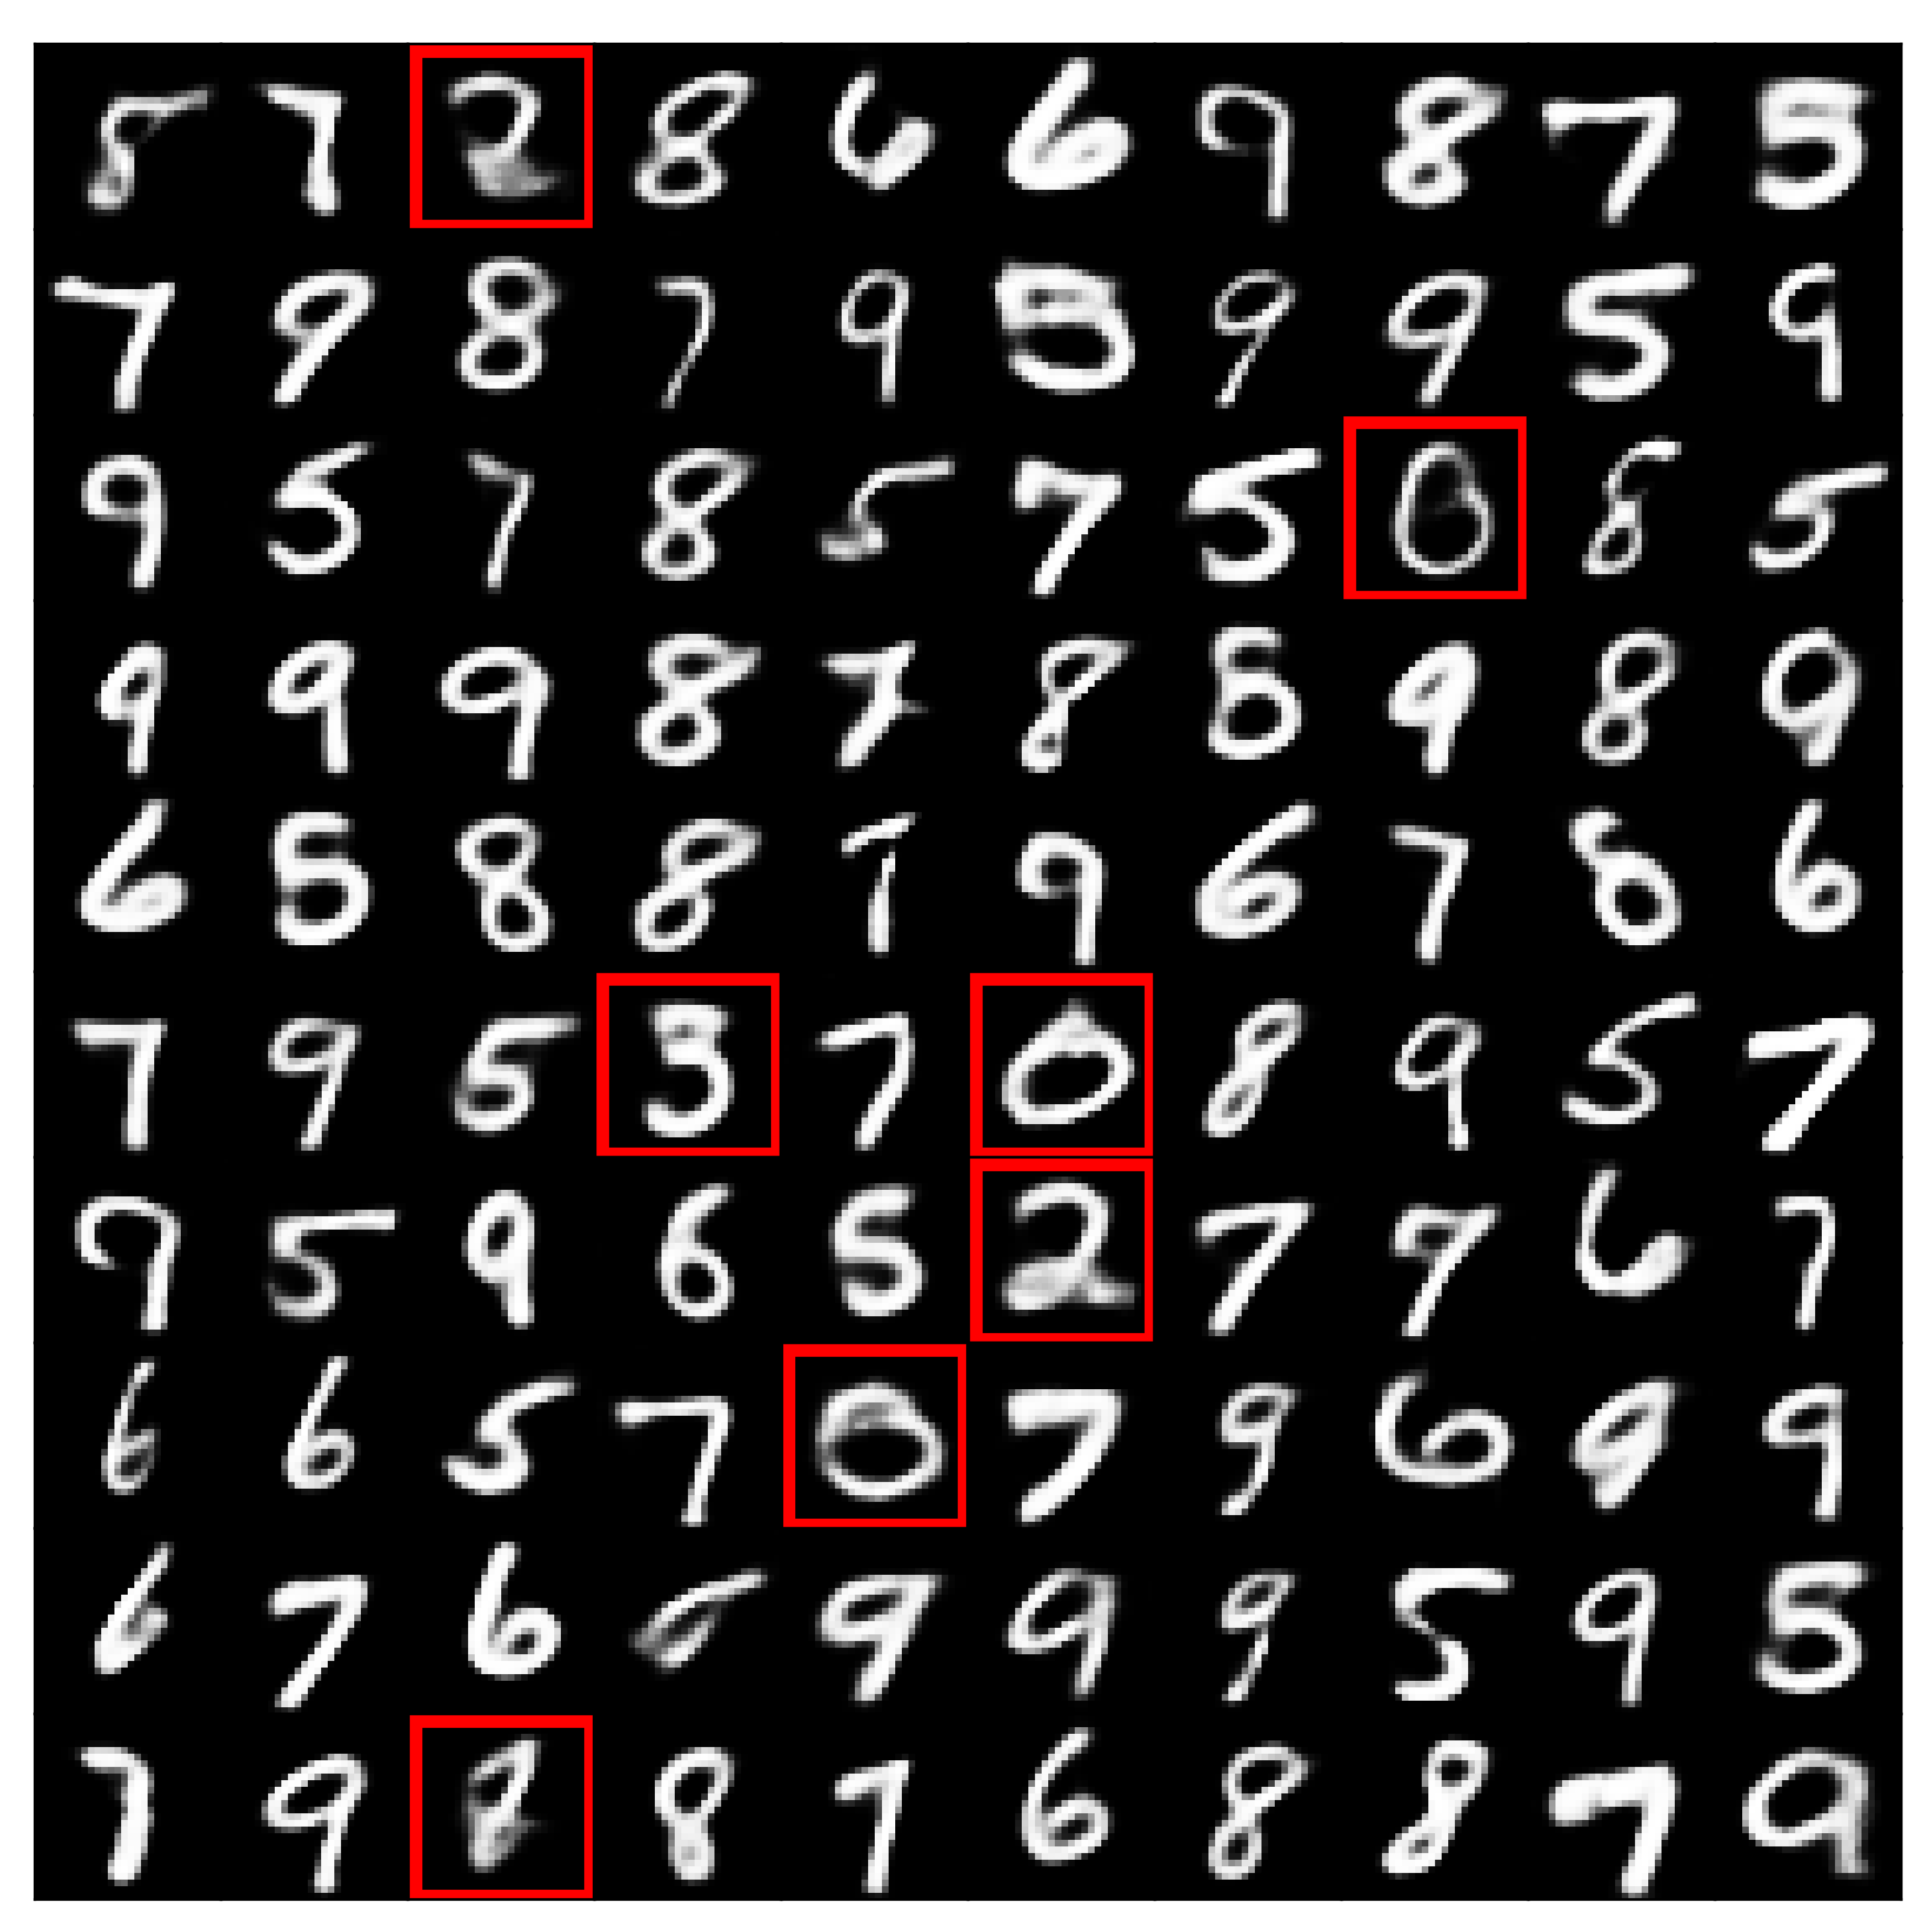
\includegraphics[width=0.7\textwidth]{Figures/Methods/ub09_random_generation.png}
    \end{subfigure}
    \hfill
    \begin{subfigure}{0.45\textwidth}
        \centering
        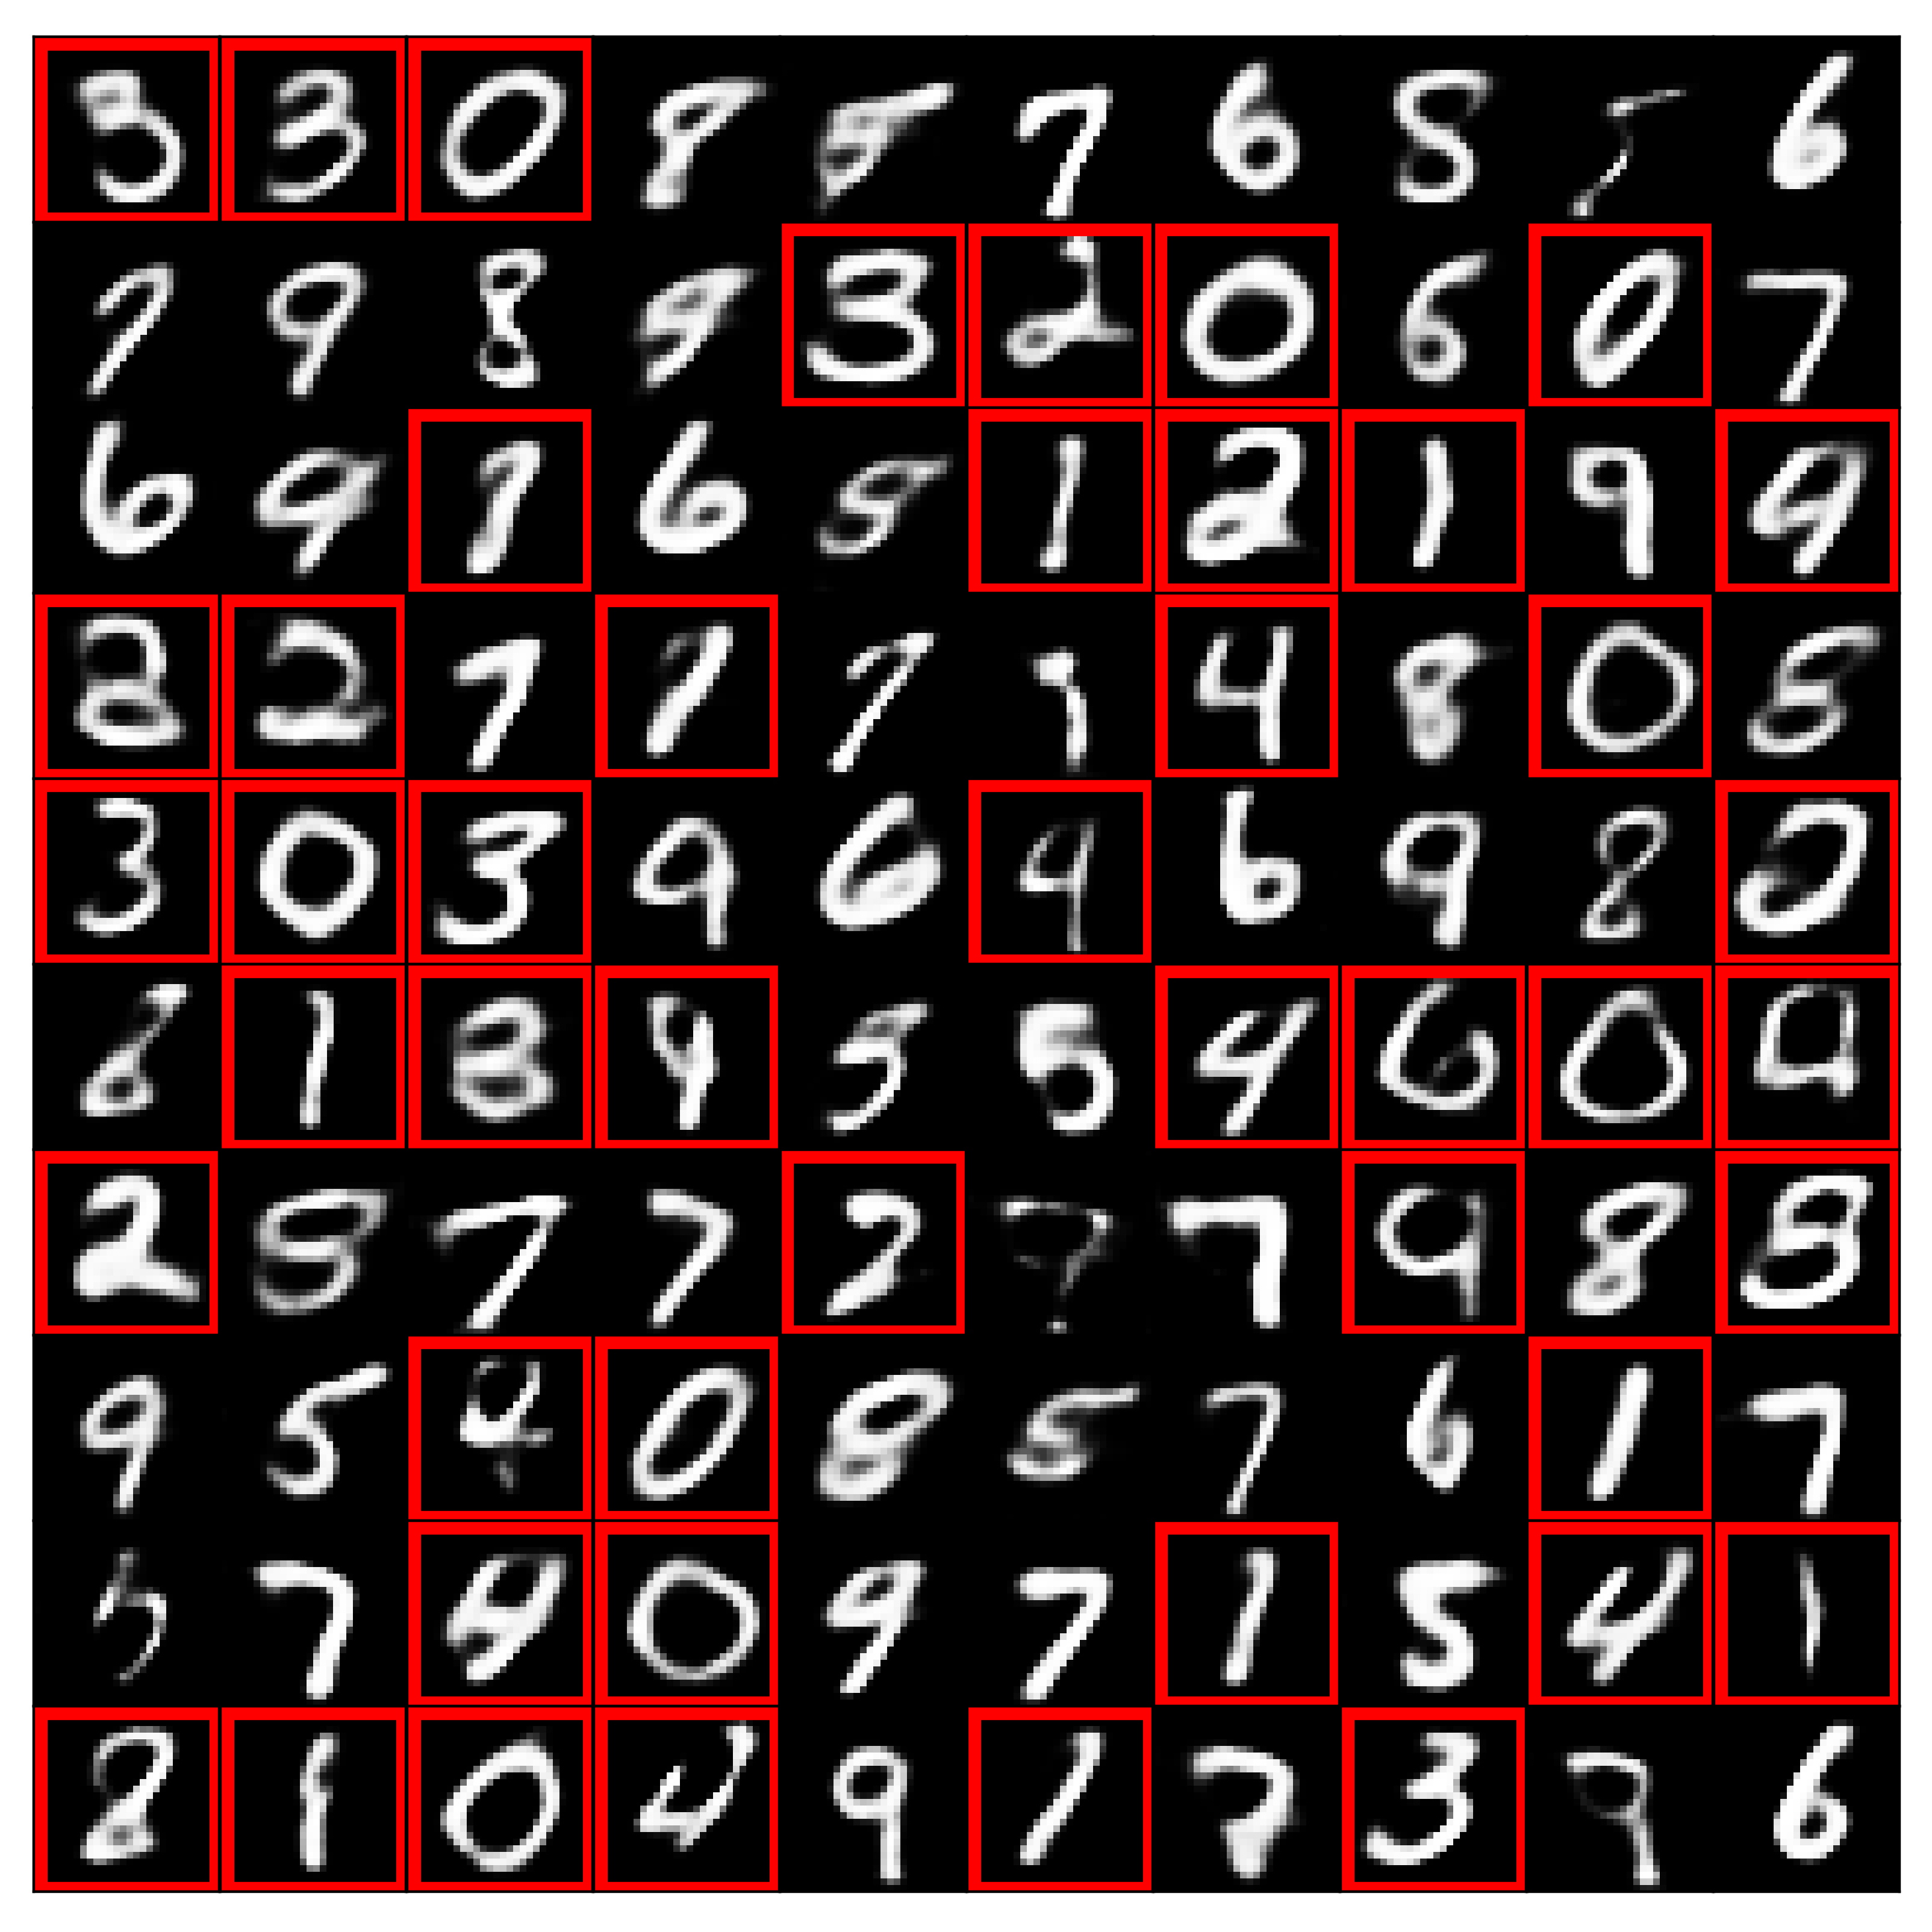
\includegraphics[width=0.7\textwidth]{Figures/Methods/invw_ub09_random_generation.png}
    \end{subfigure}
    \hfill
    \begin{subfigure}{0.45\textwidth}
        \centering
        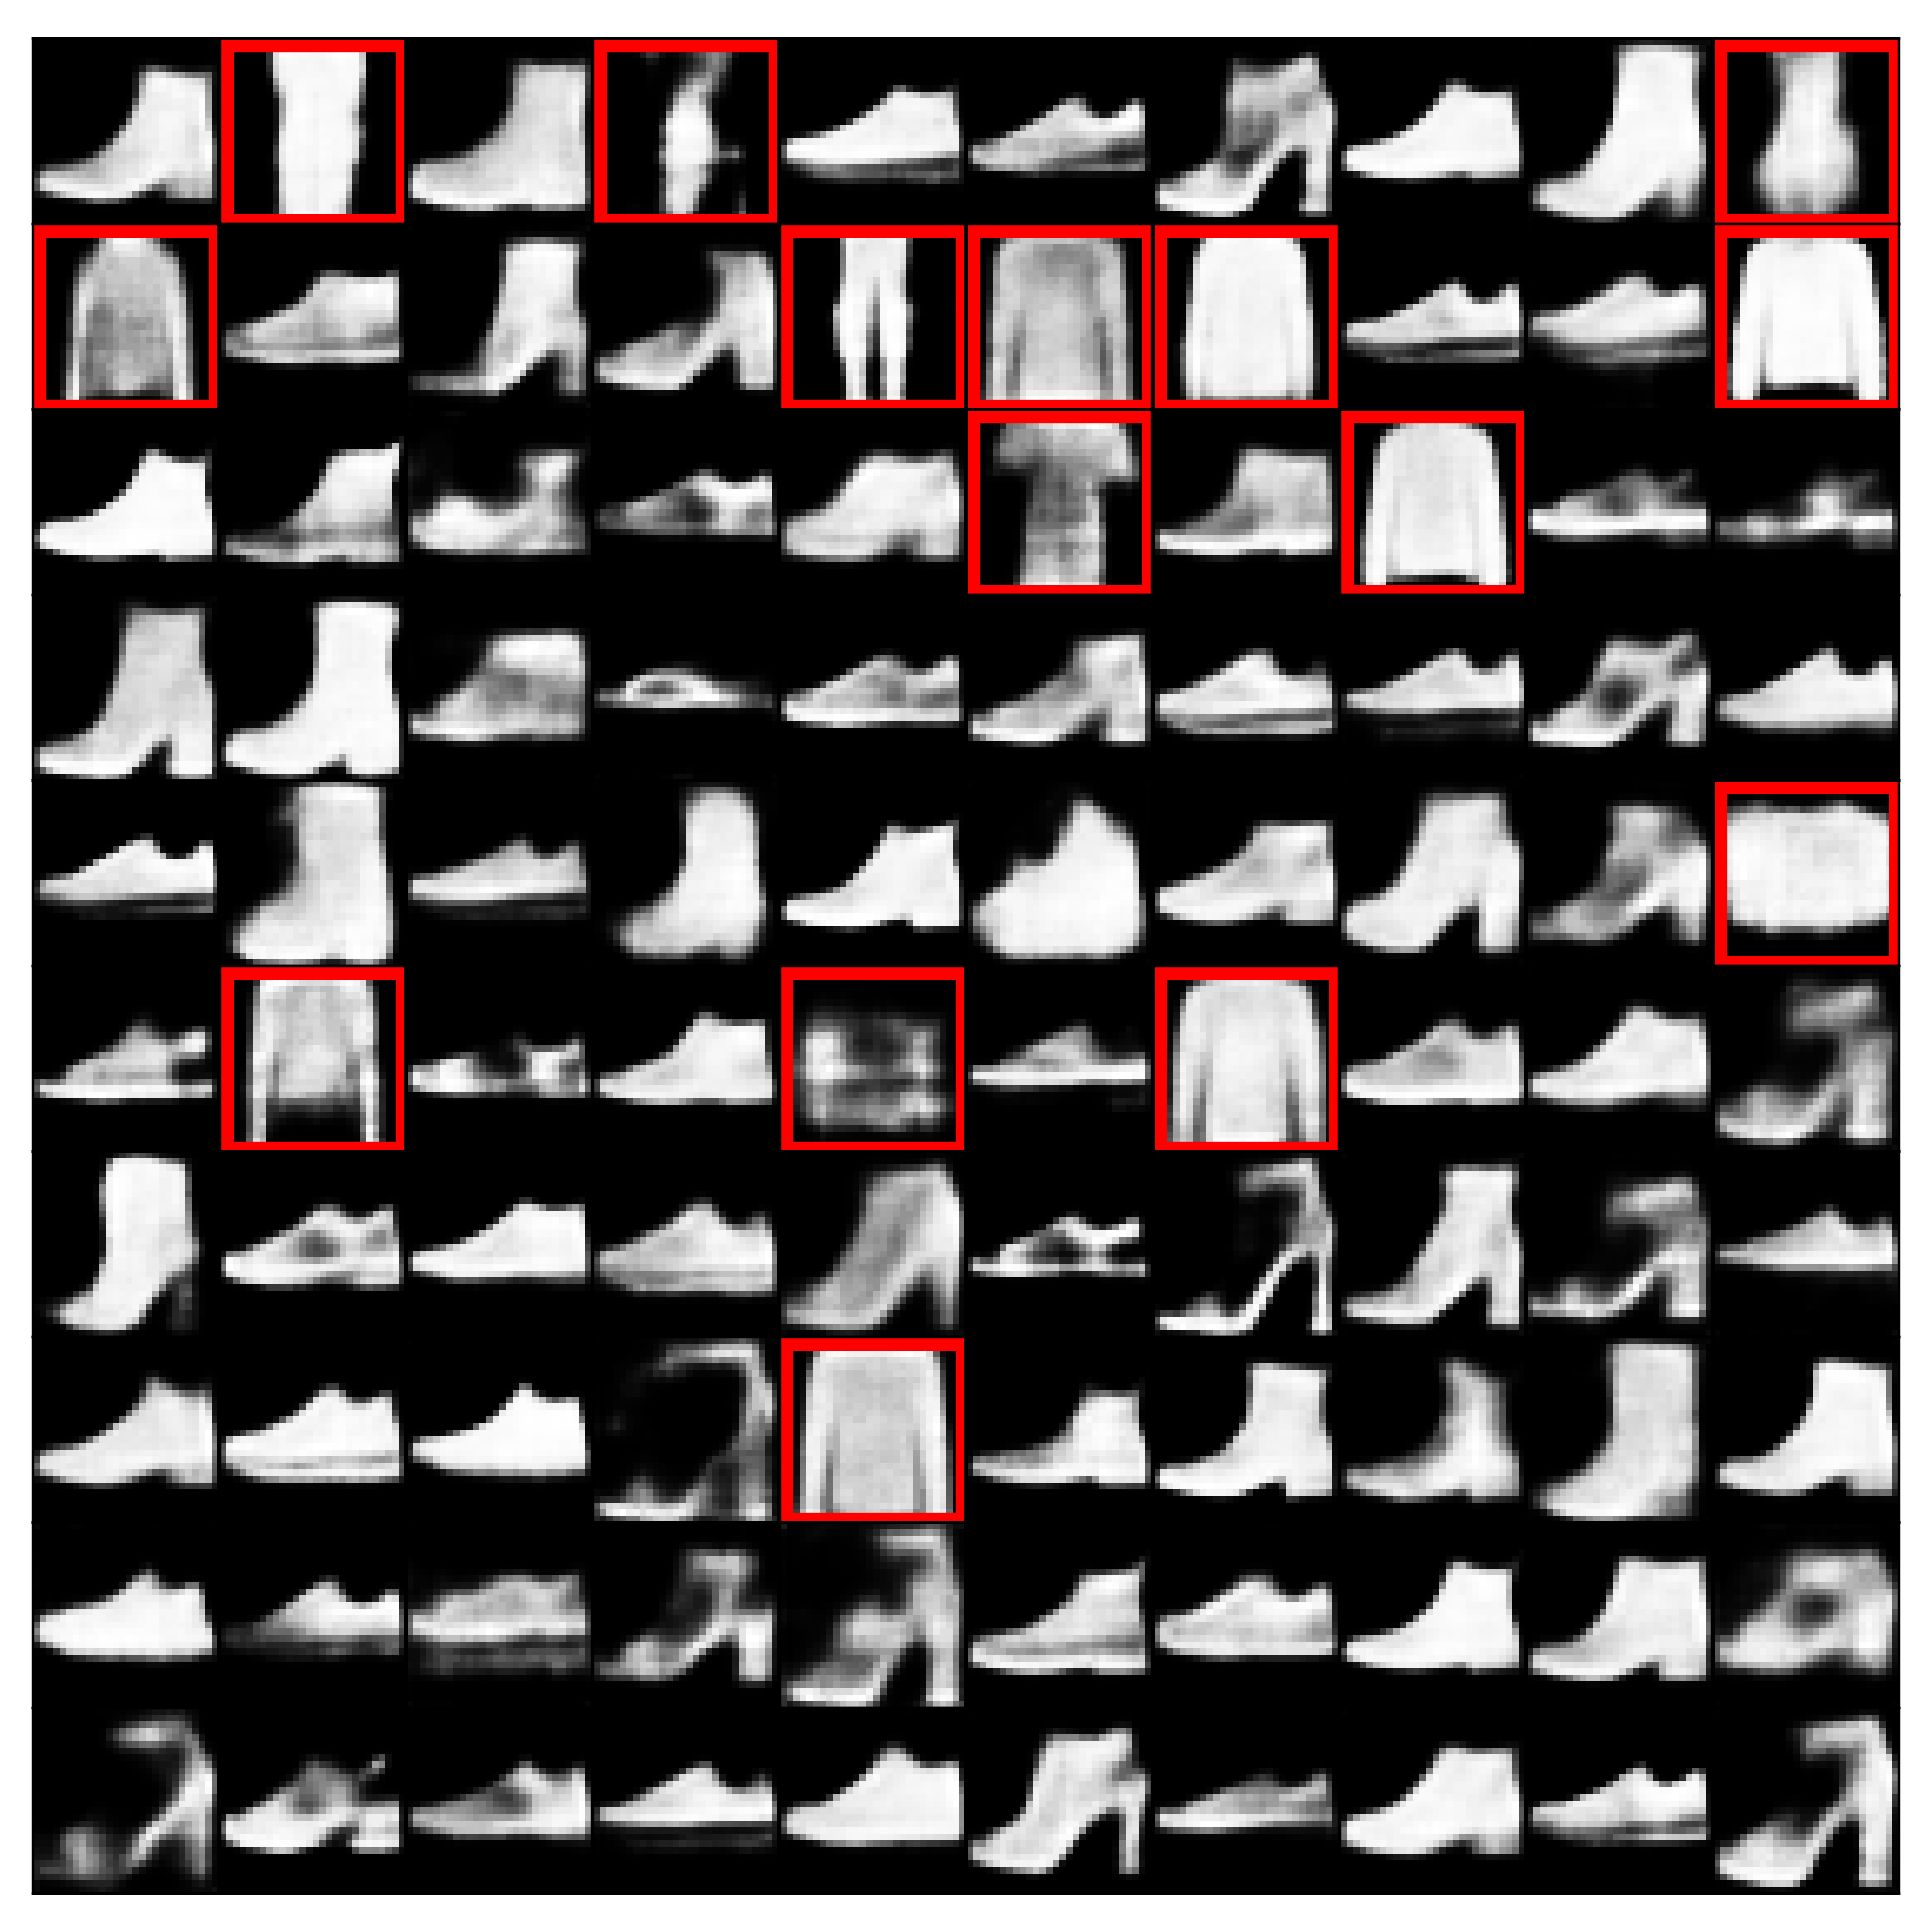
\includegraphics[width=0.7\textwidth]{Figures/Methods/FSM_random_generation.png}
    \end{subfigure}
    \hfill
    \begin{subfigure}{0.45\textwidth}
        \centering
        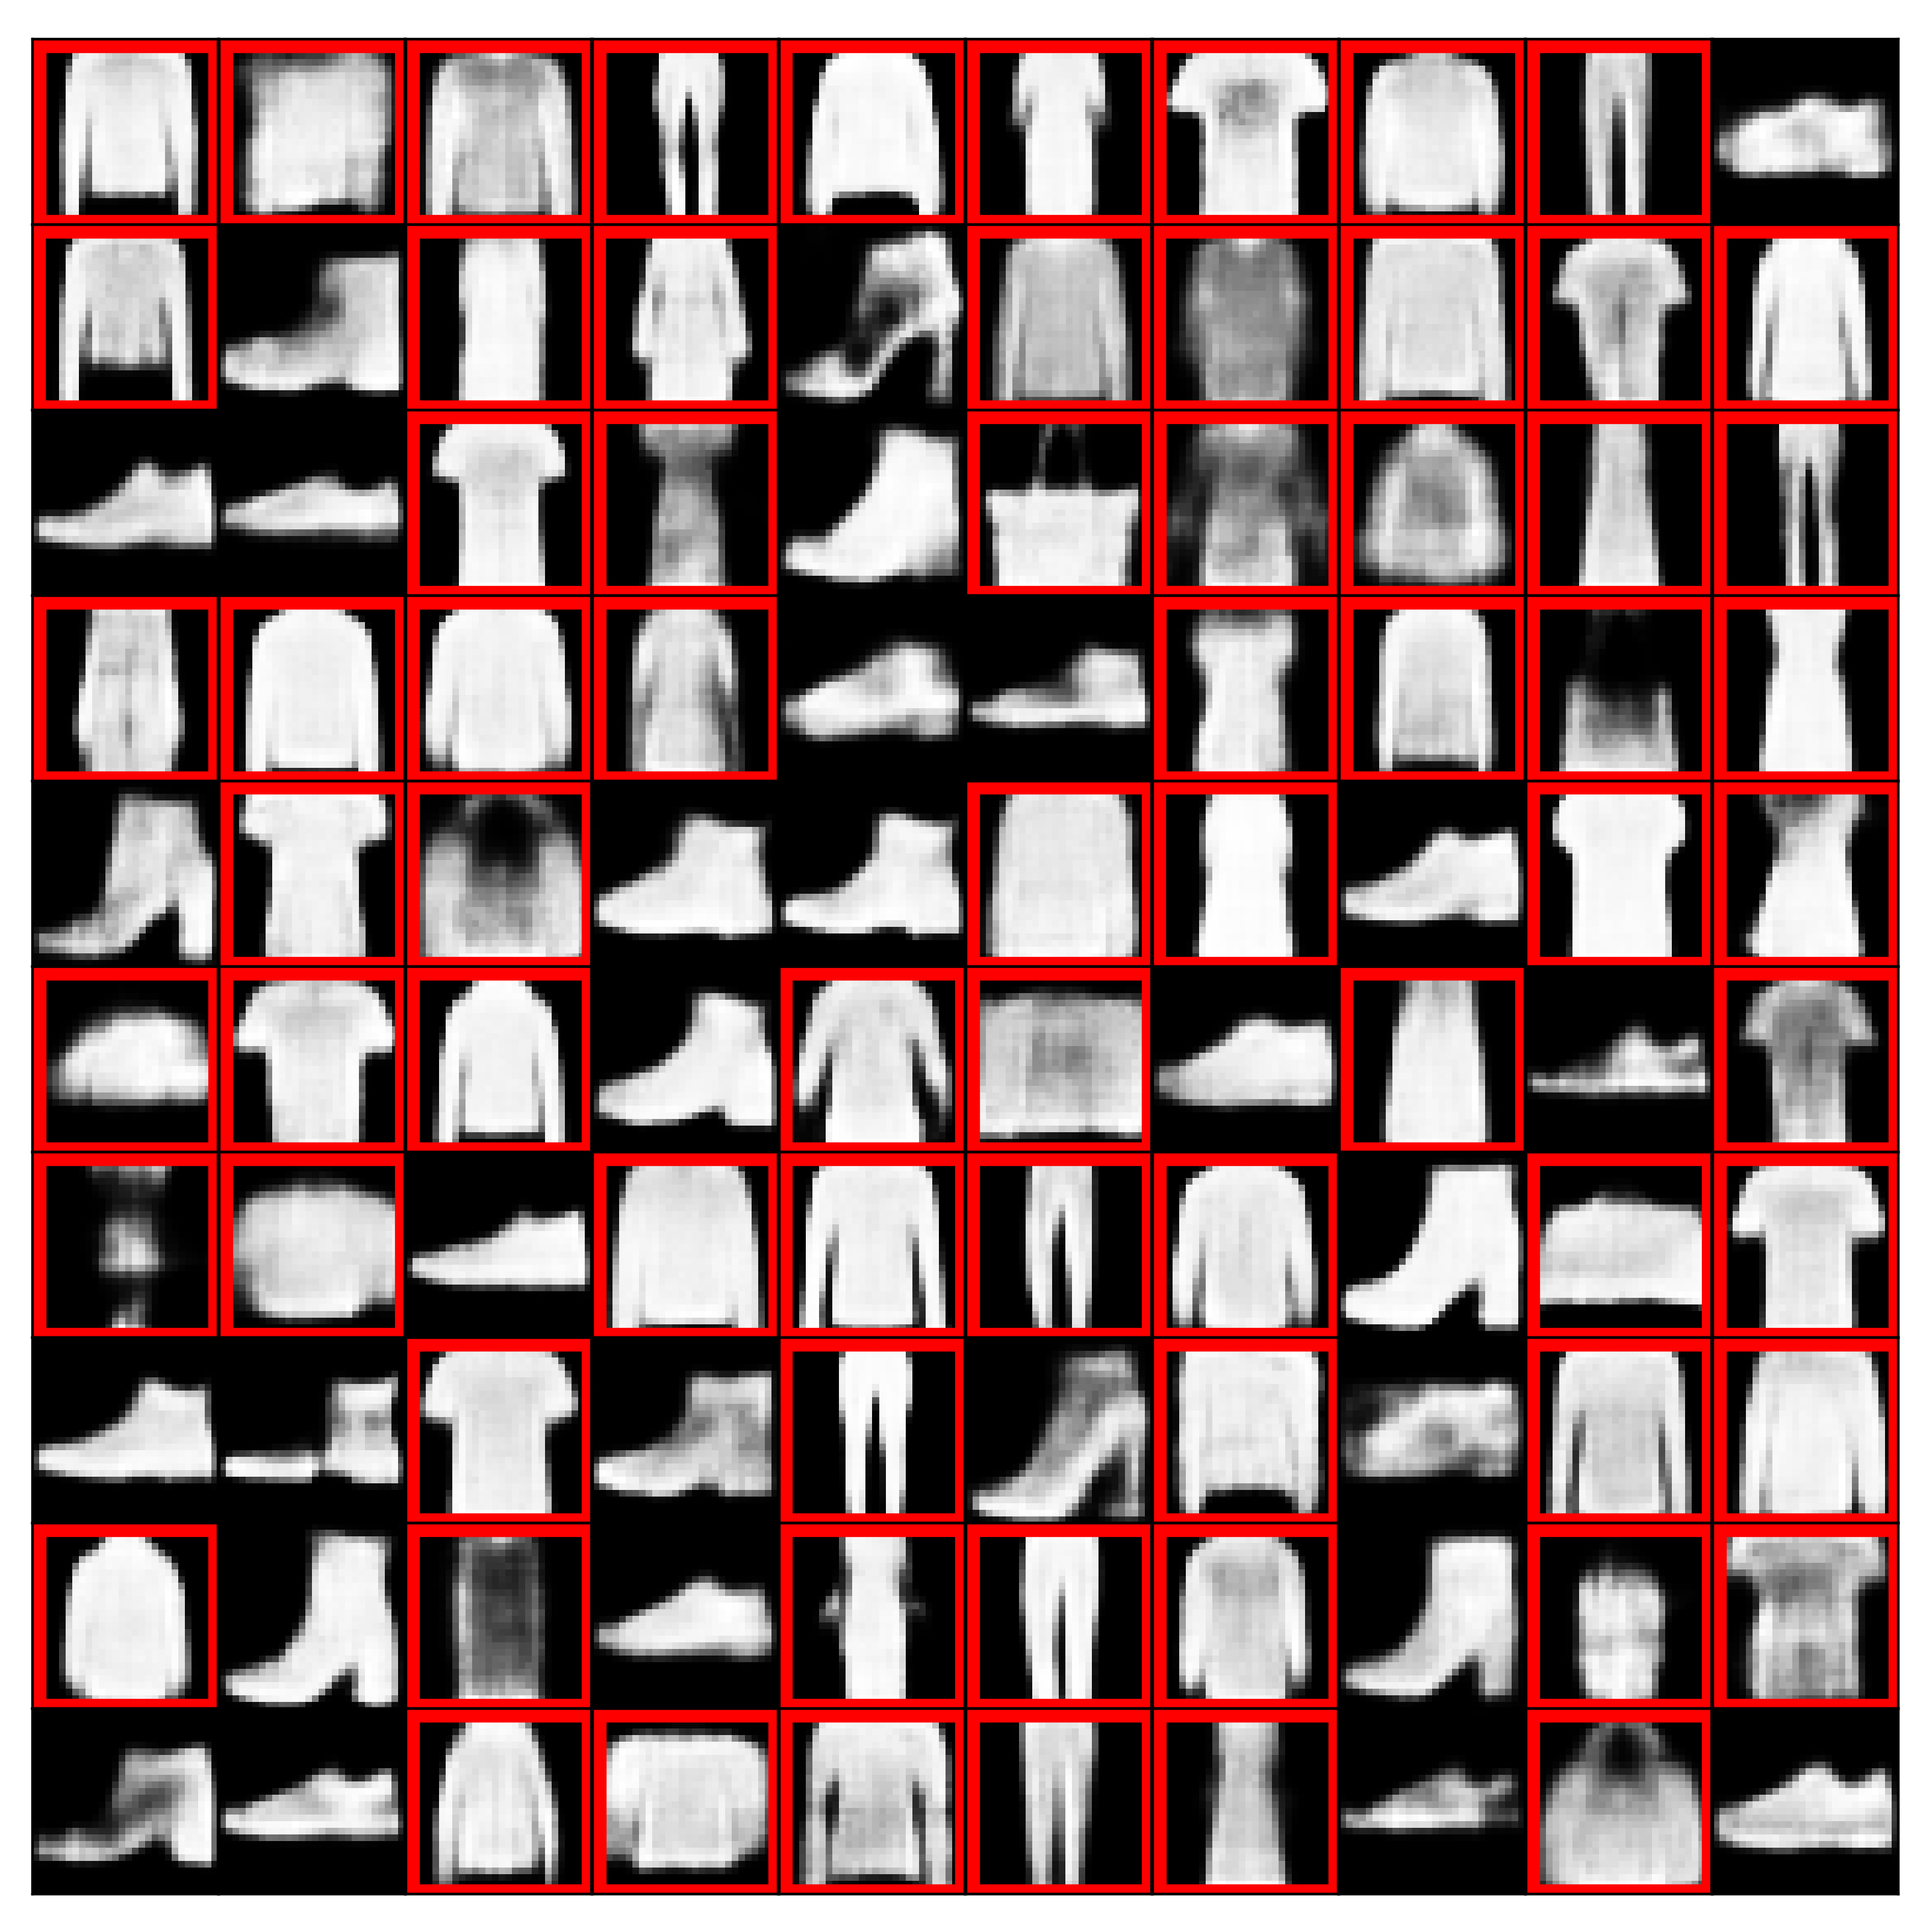
\includegraphics[width=0.7\textwidth]{Figures/Methods/FSM_invw_random_generation.png}
    \end{subfigure}
    \caption{Random generation of unbalanced MNIST dataset: vanilla Gen-RKM (top right) and Gen-RKM with inverse frequency sampling (top left). Fashion MNIST dataset: vanilla Gen-RKM (down right) and Gen-RKM with inverse frequency sampling (down left)}
    \label{fig-ub09}
\end{figure}


% \begin{figure}[H]
%     \centering
%     \begin{subfigure}{0.45\textwidth}
%         \centering
%         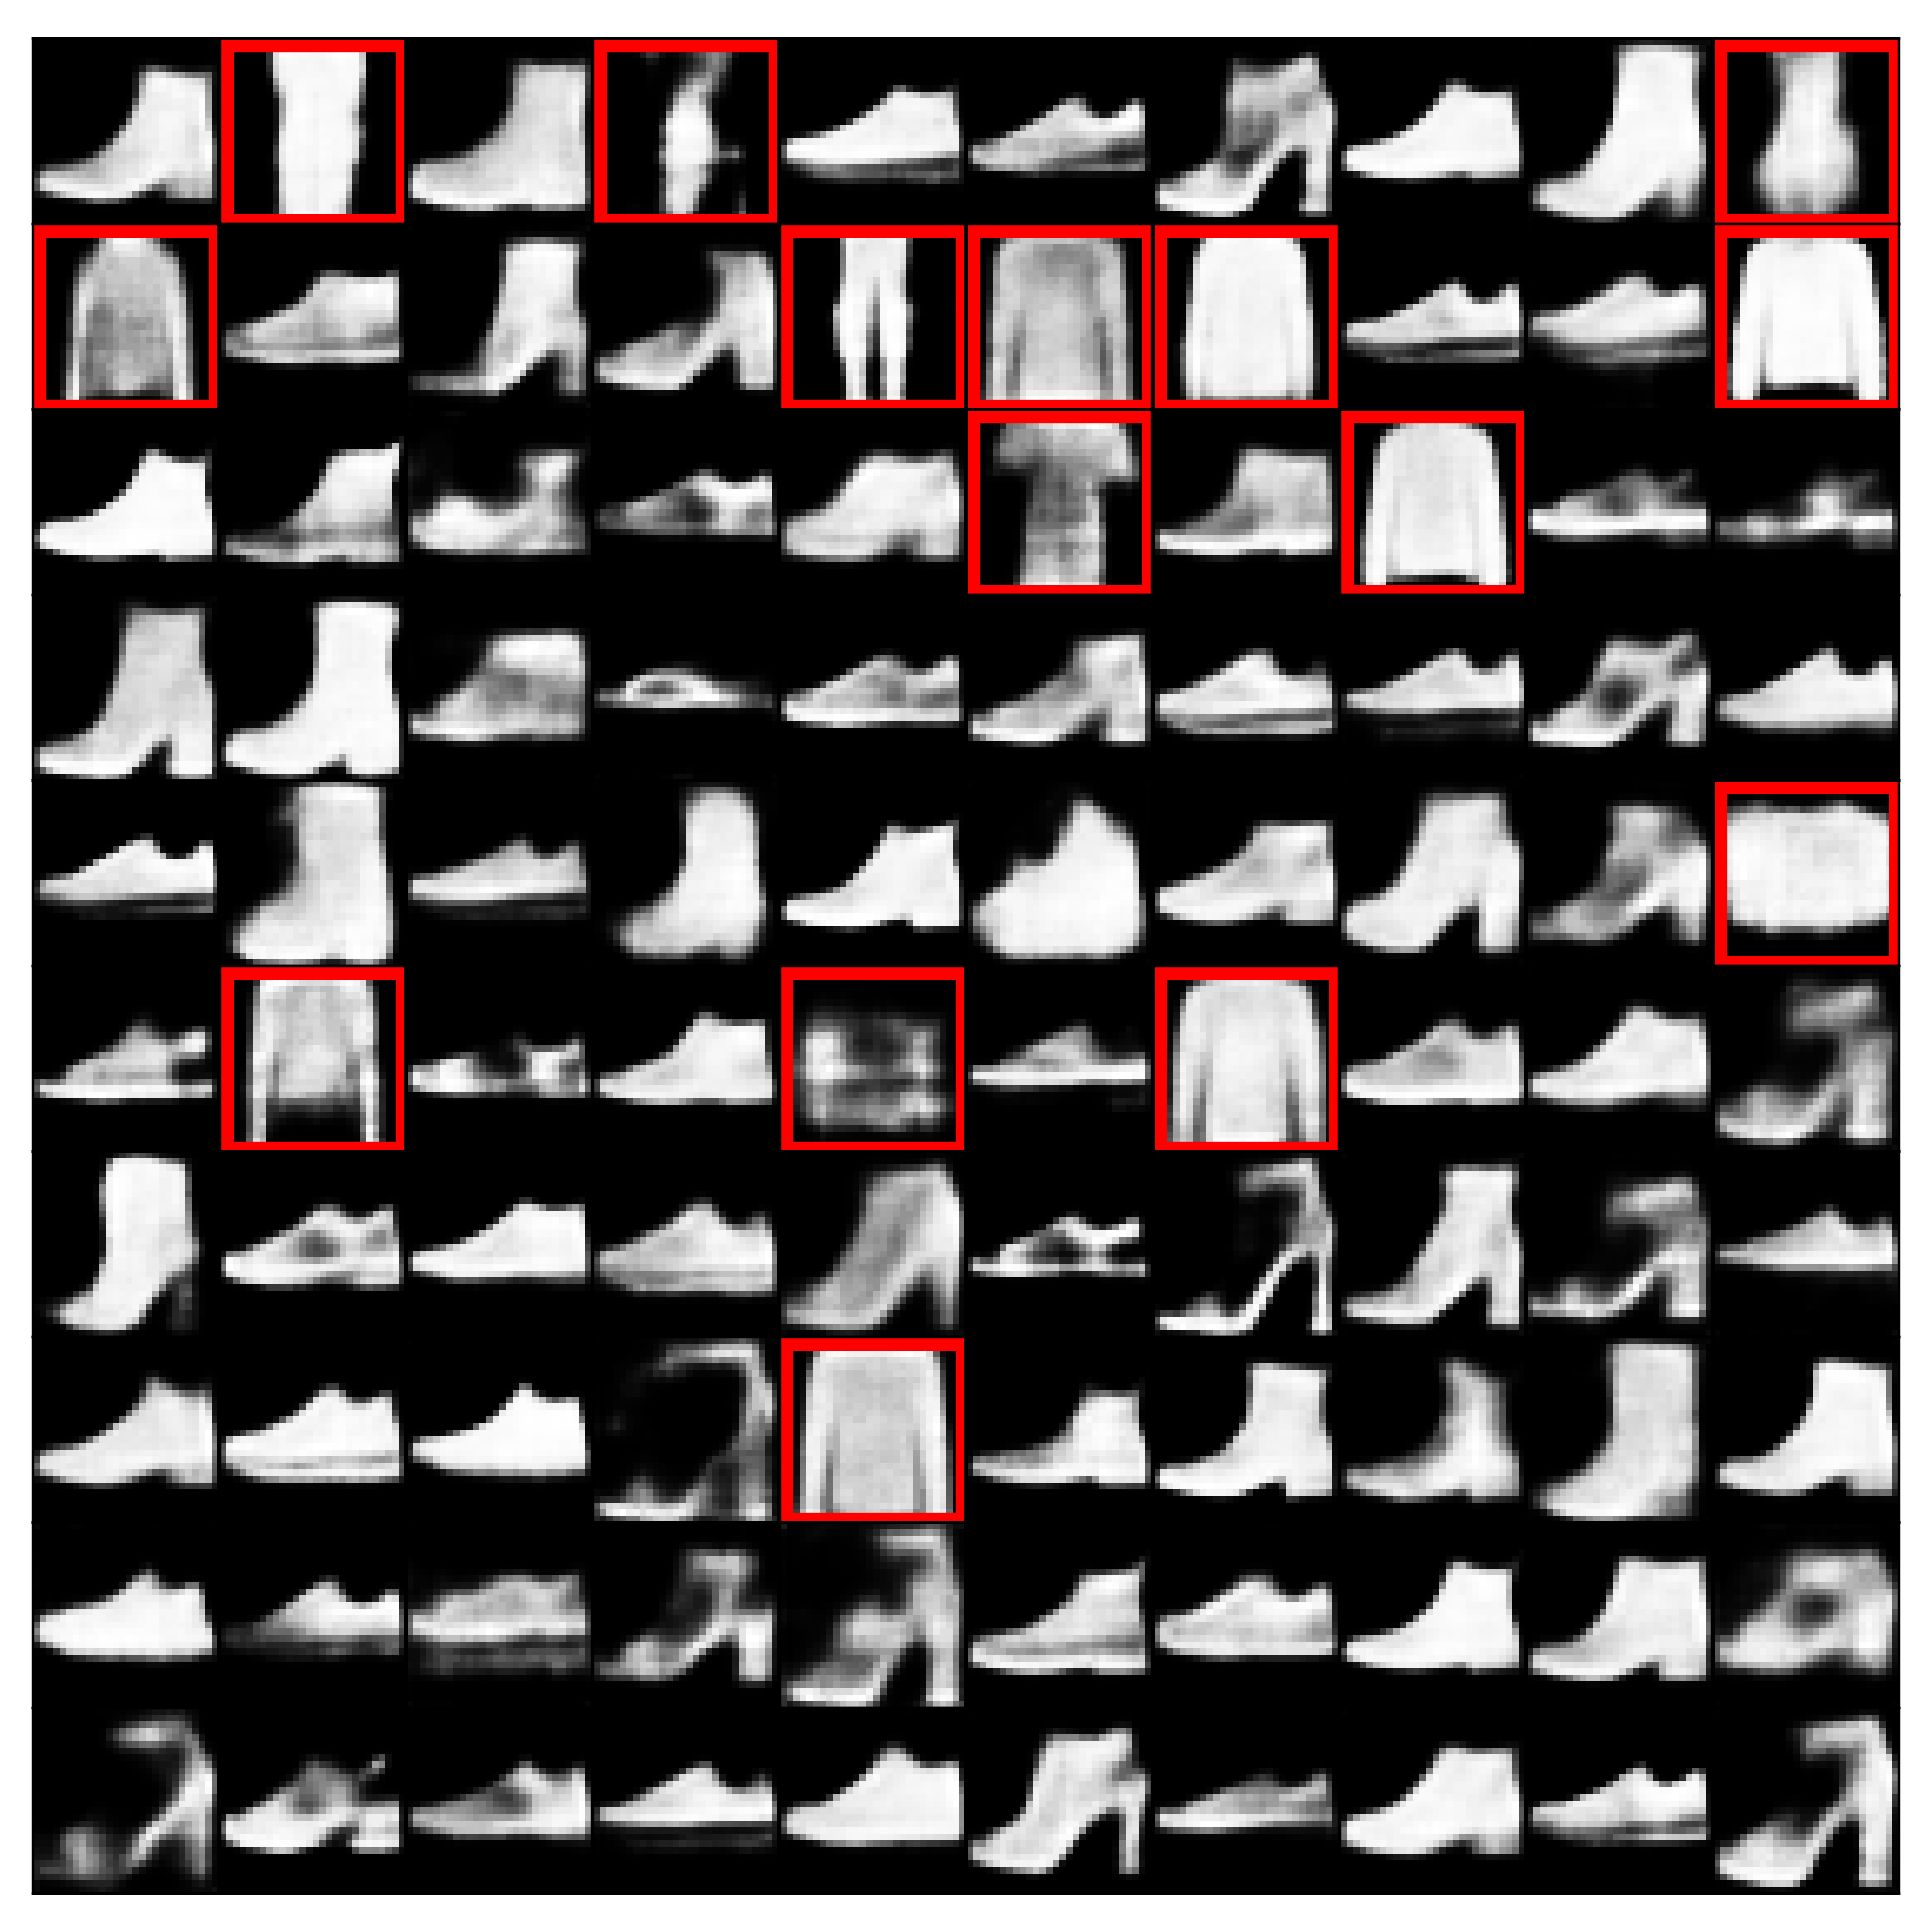
\includegraphics[width=0.8\textwidth]{Figures/Methods/FSM_random_generation.png}
%     \end{subfigure}
%     \hfill
%     \begin{subfigure}{0.45\textwidth}
%         \centering
%         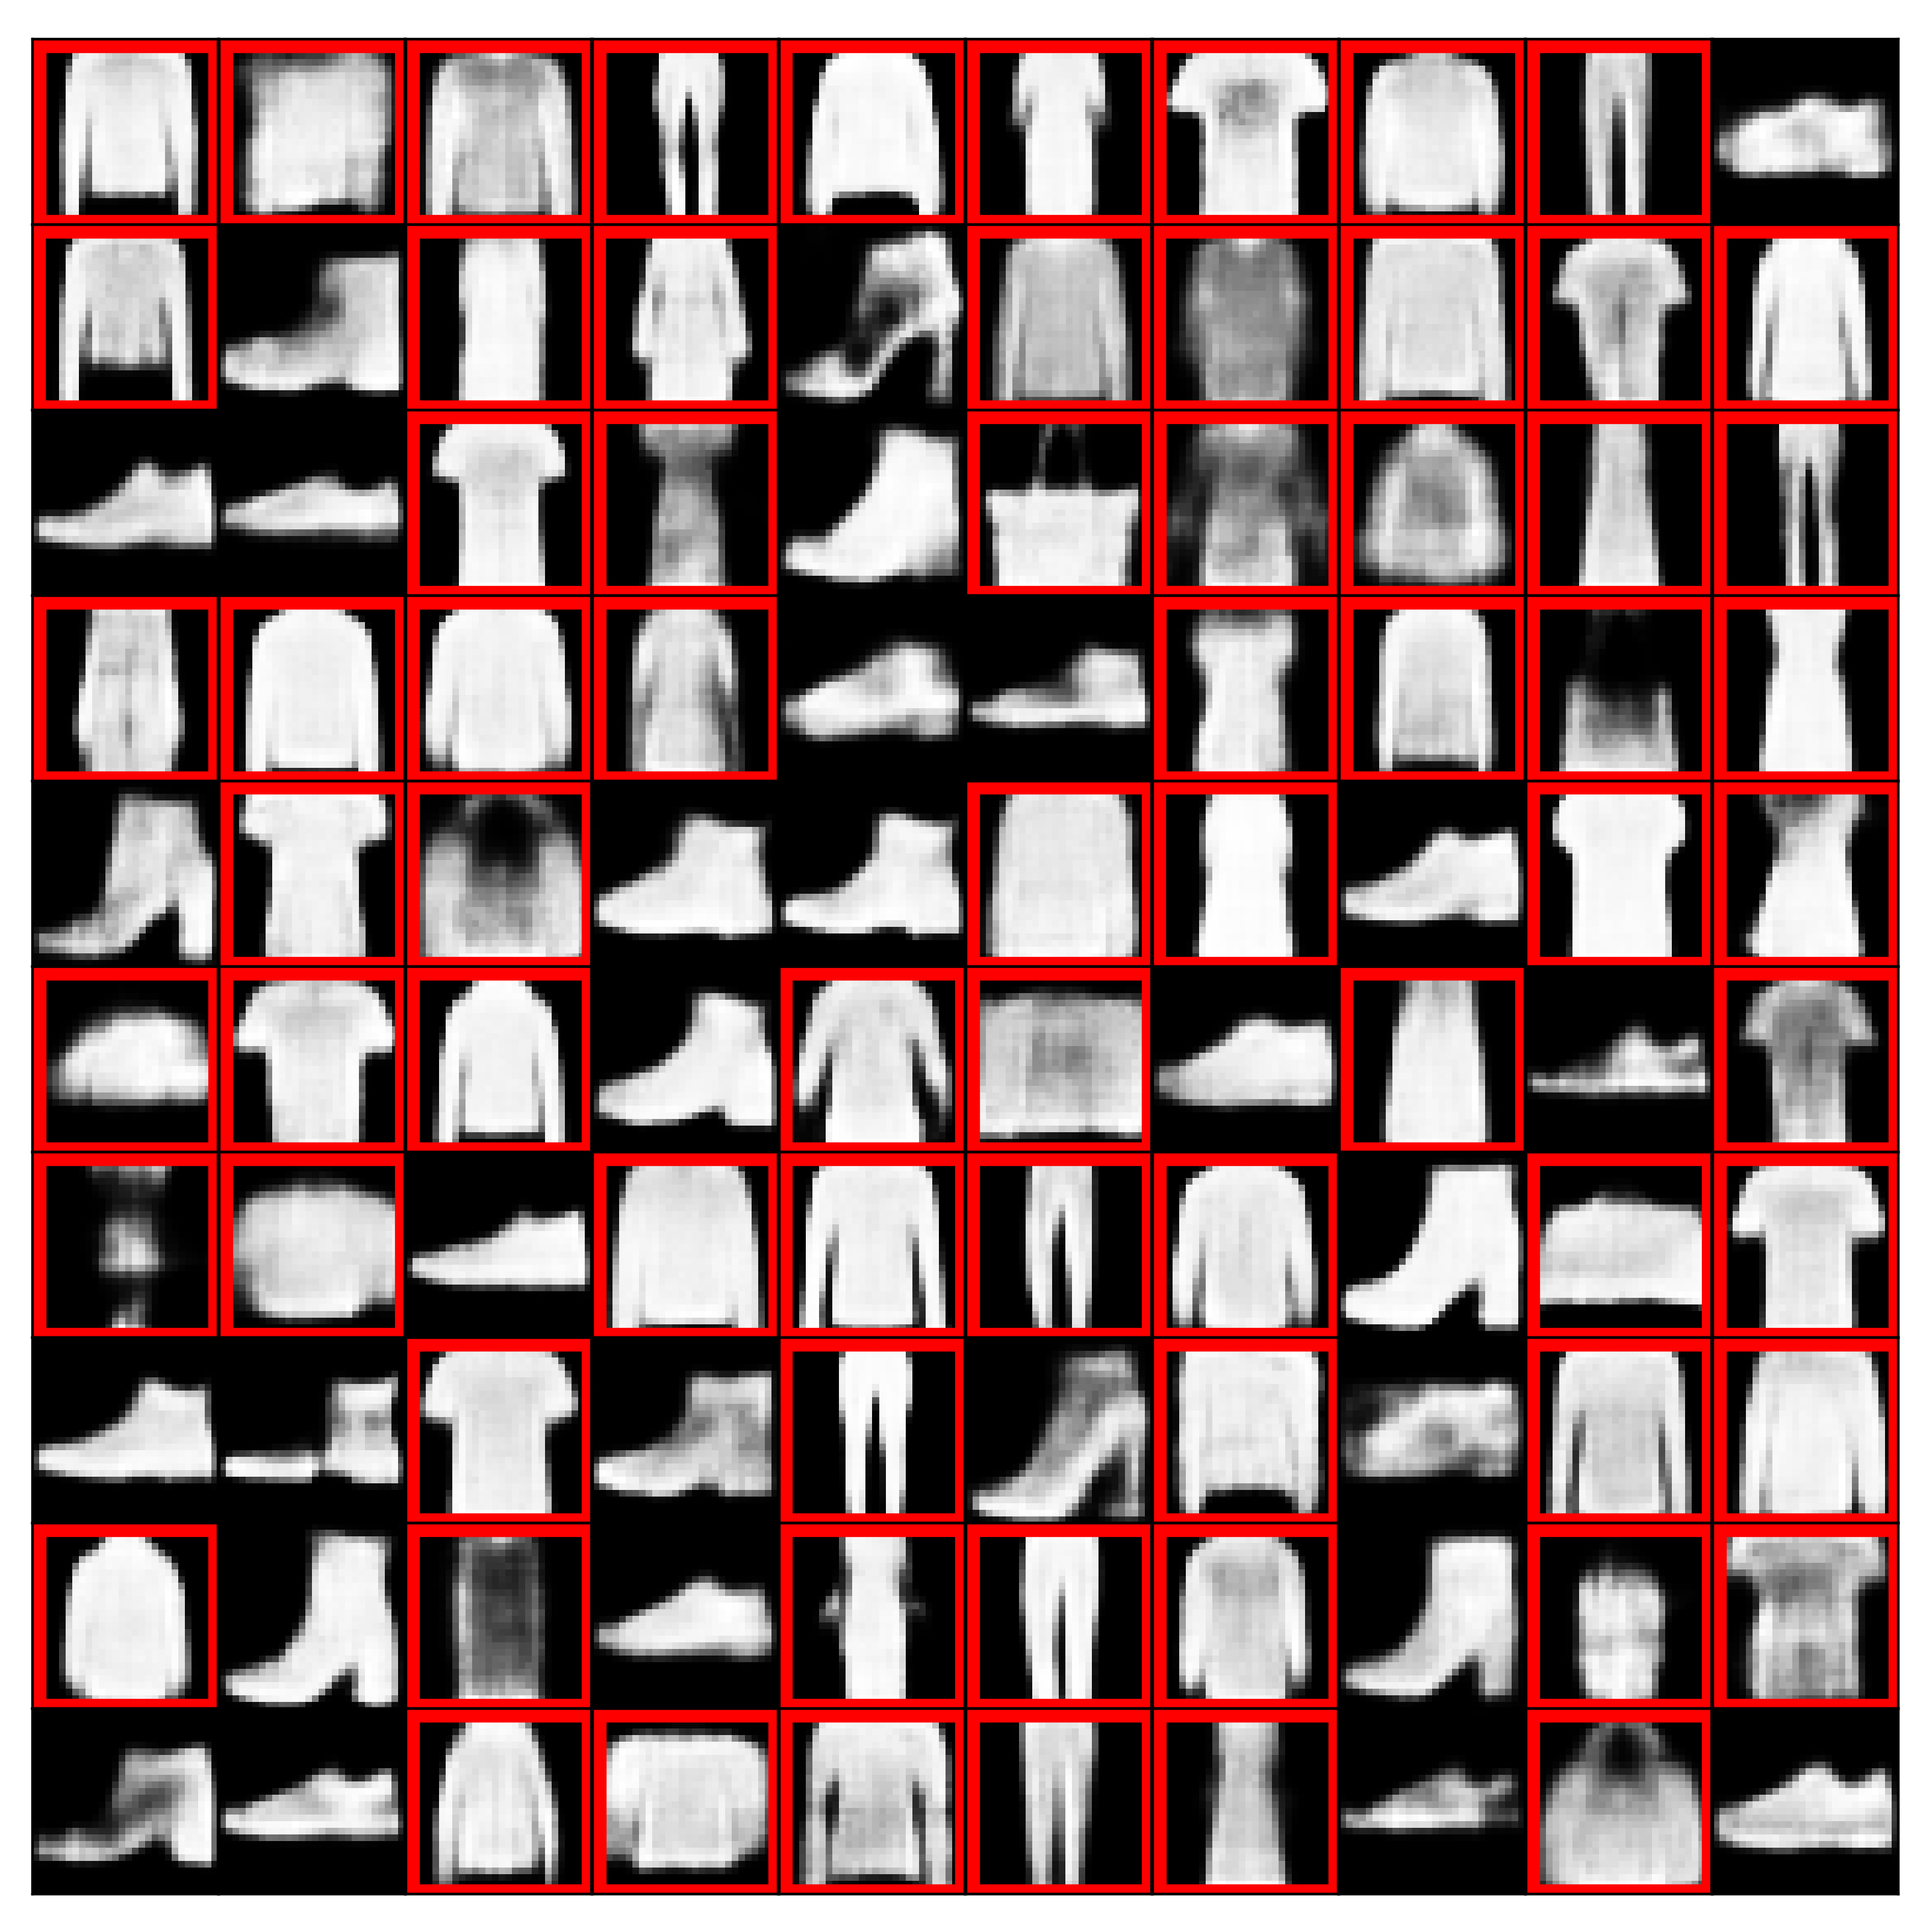
\includegraphics[width=0.8\textwidth]{Figures/Methods/FSM_invw_random_generation.png}
%     \end{subfigure}
%     \caption{Random generation of unbalanced FashionMNIST dataset: vanilla Gen-RKM (right) and Gen-RKM with inverse frequency sampling (left)}
%     \label{fig-ubfs}
% \end{figure}

\subsection{Effect of inverse frequency sampling on conditional generation in Gen-RKM}
We examine the effectiveness of conditional generation (described in Section \ref{subsec-methods-congen}) within the framework of Gen-RKM in this section. Conditional generations on unbalanced MNIST and unbalanced Fashion MNIST are visualized in Figure \ref{fig-IWS-congen}. Unsurprisingly, the generation quality could be worse if the generation is conditioned on a minority class, and it is likely to incorrectly generate images from other classes. For example, if one inspects the fifth column (generation conditioned on digit 4) in the MNIST case, the generation resembles digit 9 instead of digit 4. This issue is caused by the distorted latent space due to unbalanced data, latent representations of minority modes could be blurred or mixed with other majority modes, leading to failed conditional generation for underrepresented groups. This problem can now be resolved by adapting Gen-RKM with inverse frequency sampling. As shown in the right side of Figure \ref{fig-IWS-congen}, correct and clearer conditional generation can be obtained. By cleverly combining inverse frequency sampling with conditional generation, one can augment minority classes even from highly unbalanced training data.
\FloatBarrier
\begin{figure}[ht]
    \centering
    \begin{subfigure}{0.45\textwidth}
        \centering
        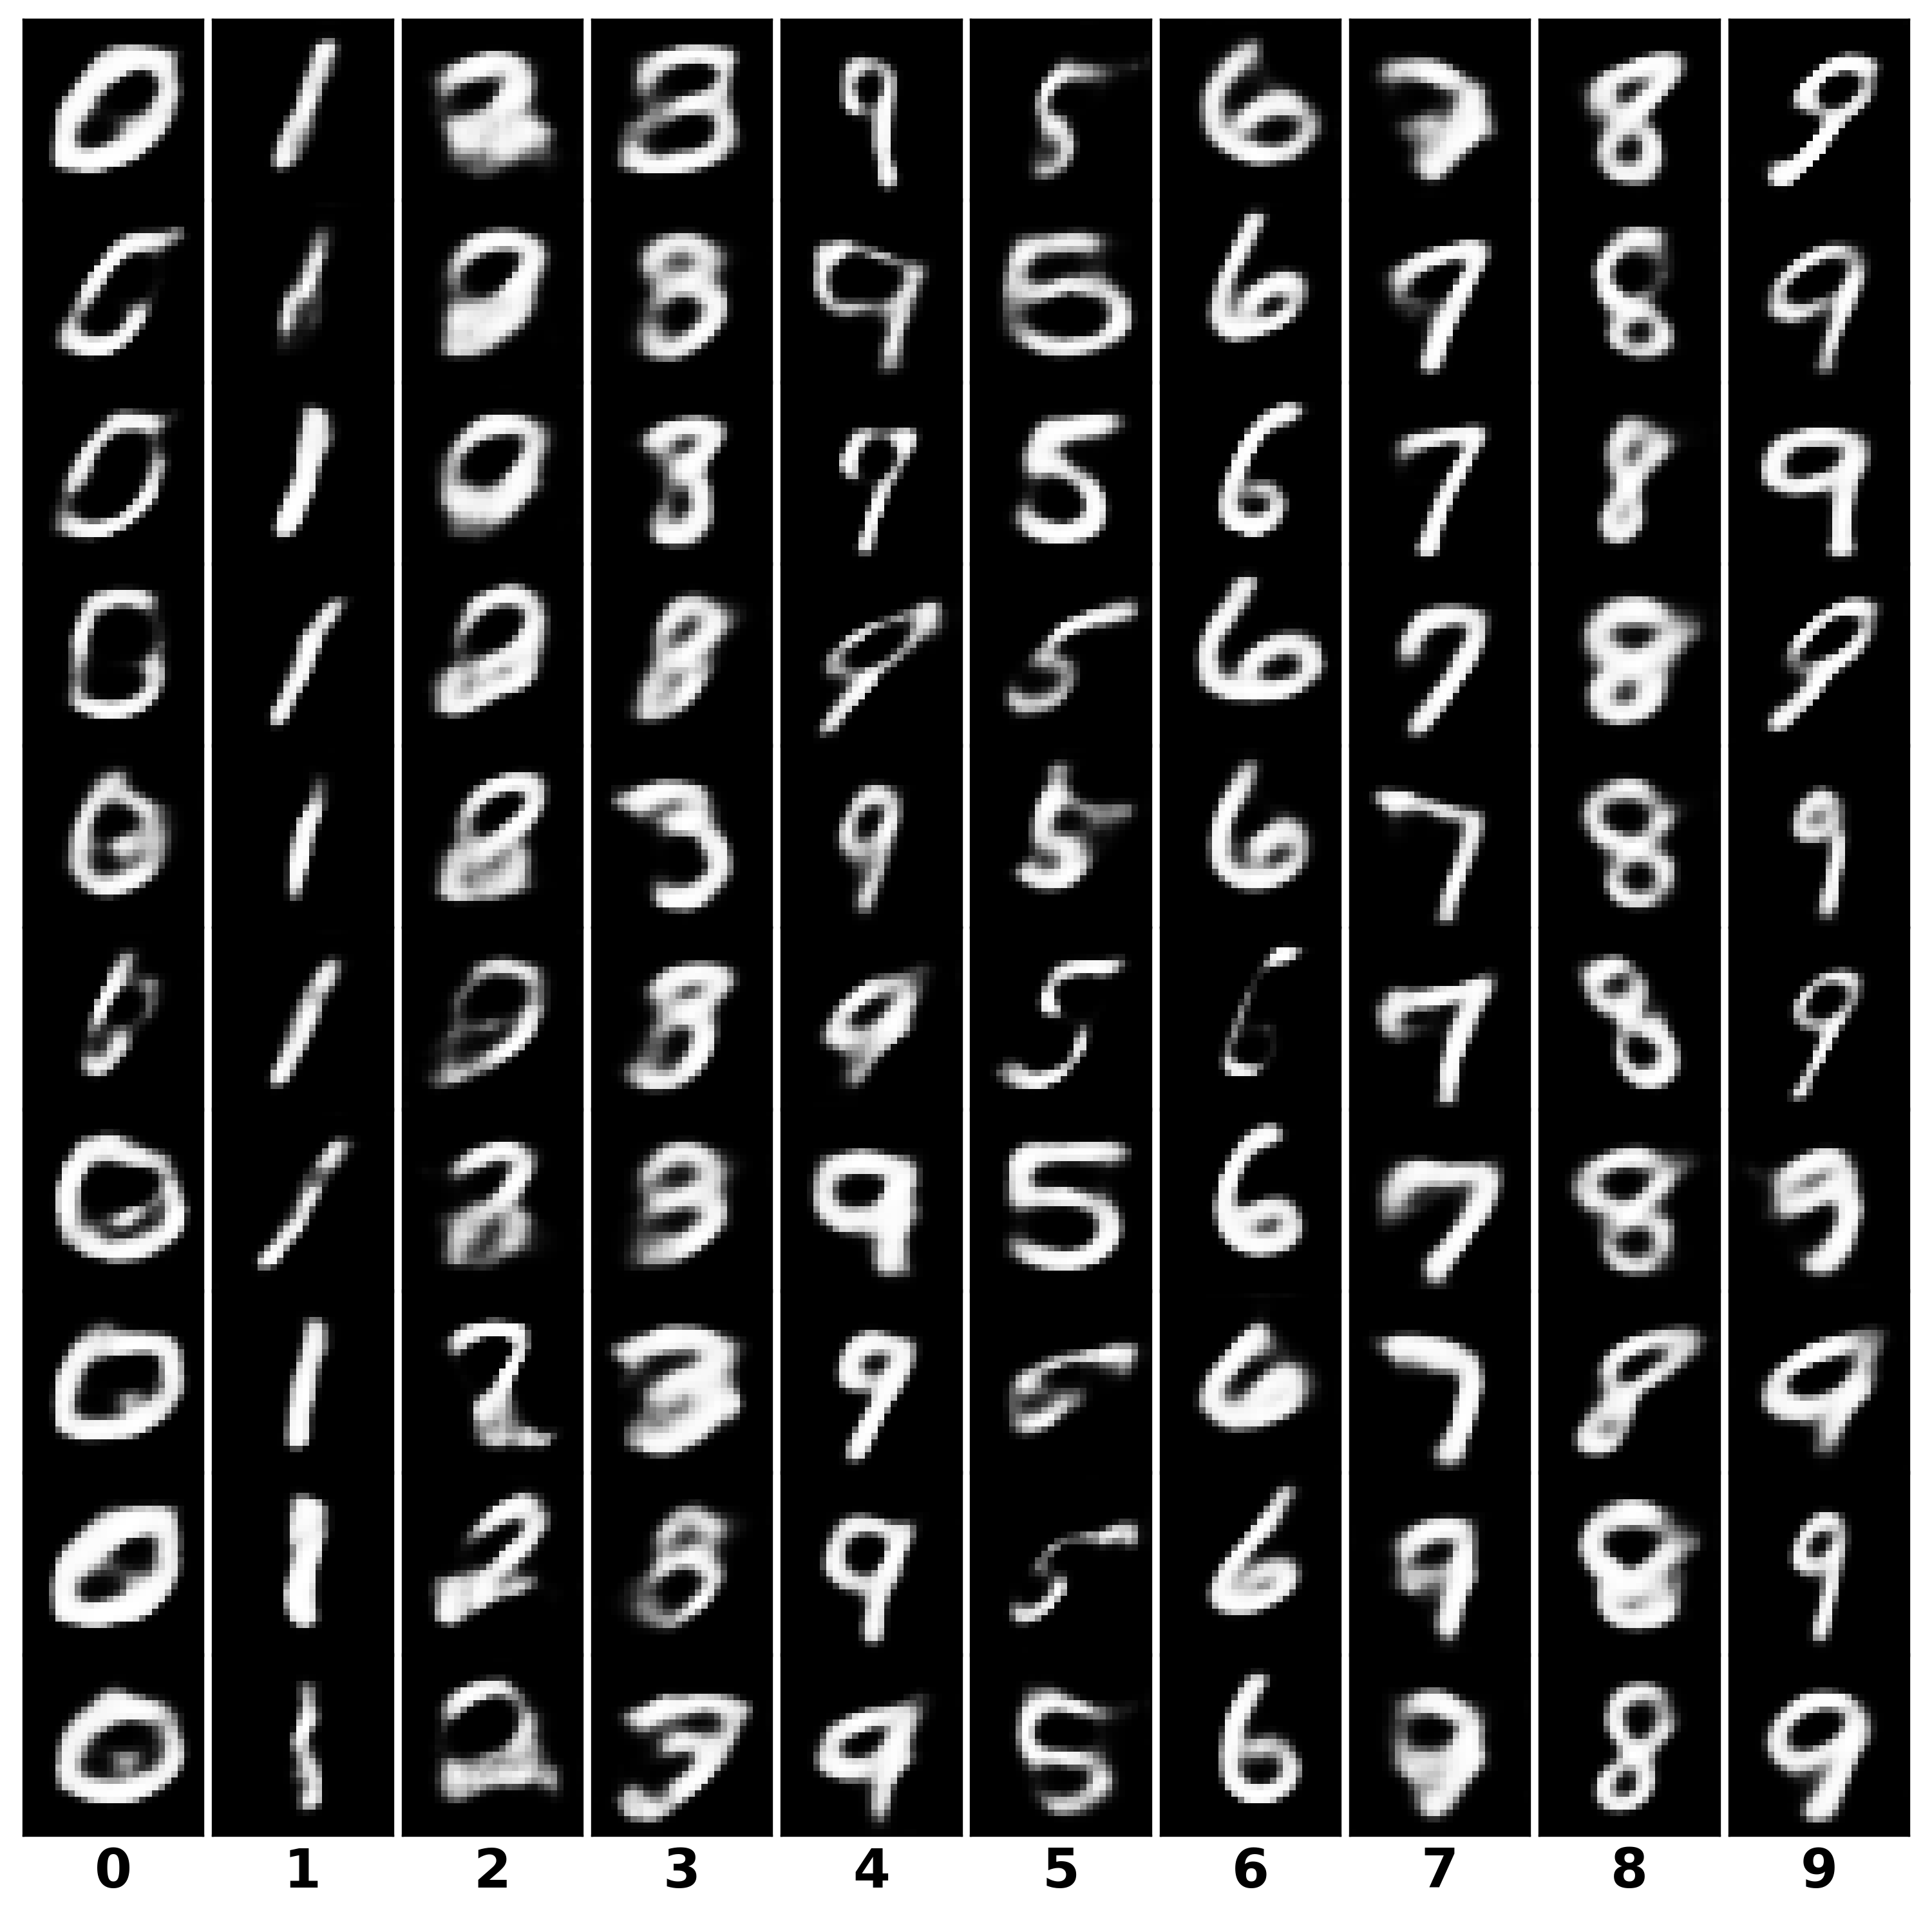
\includegraphics[width=0.7\textwidth]{Figures/Methods/RKM-congen-ubMNIST.png}
    \end{subfigure}
    \hfill
    \begin{subfigure}{0.45\textwidth}
        \centering
        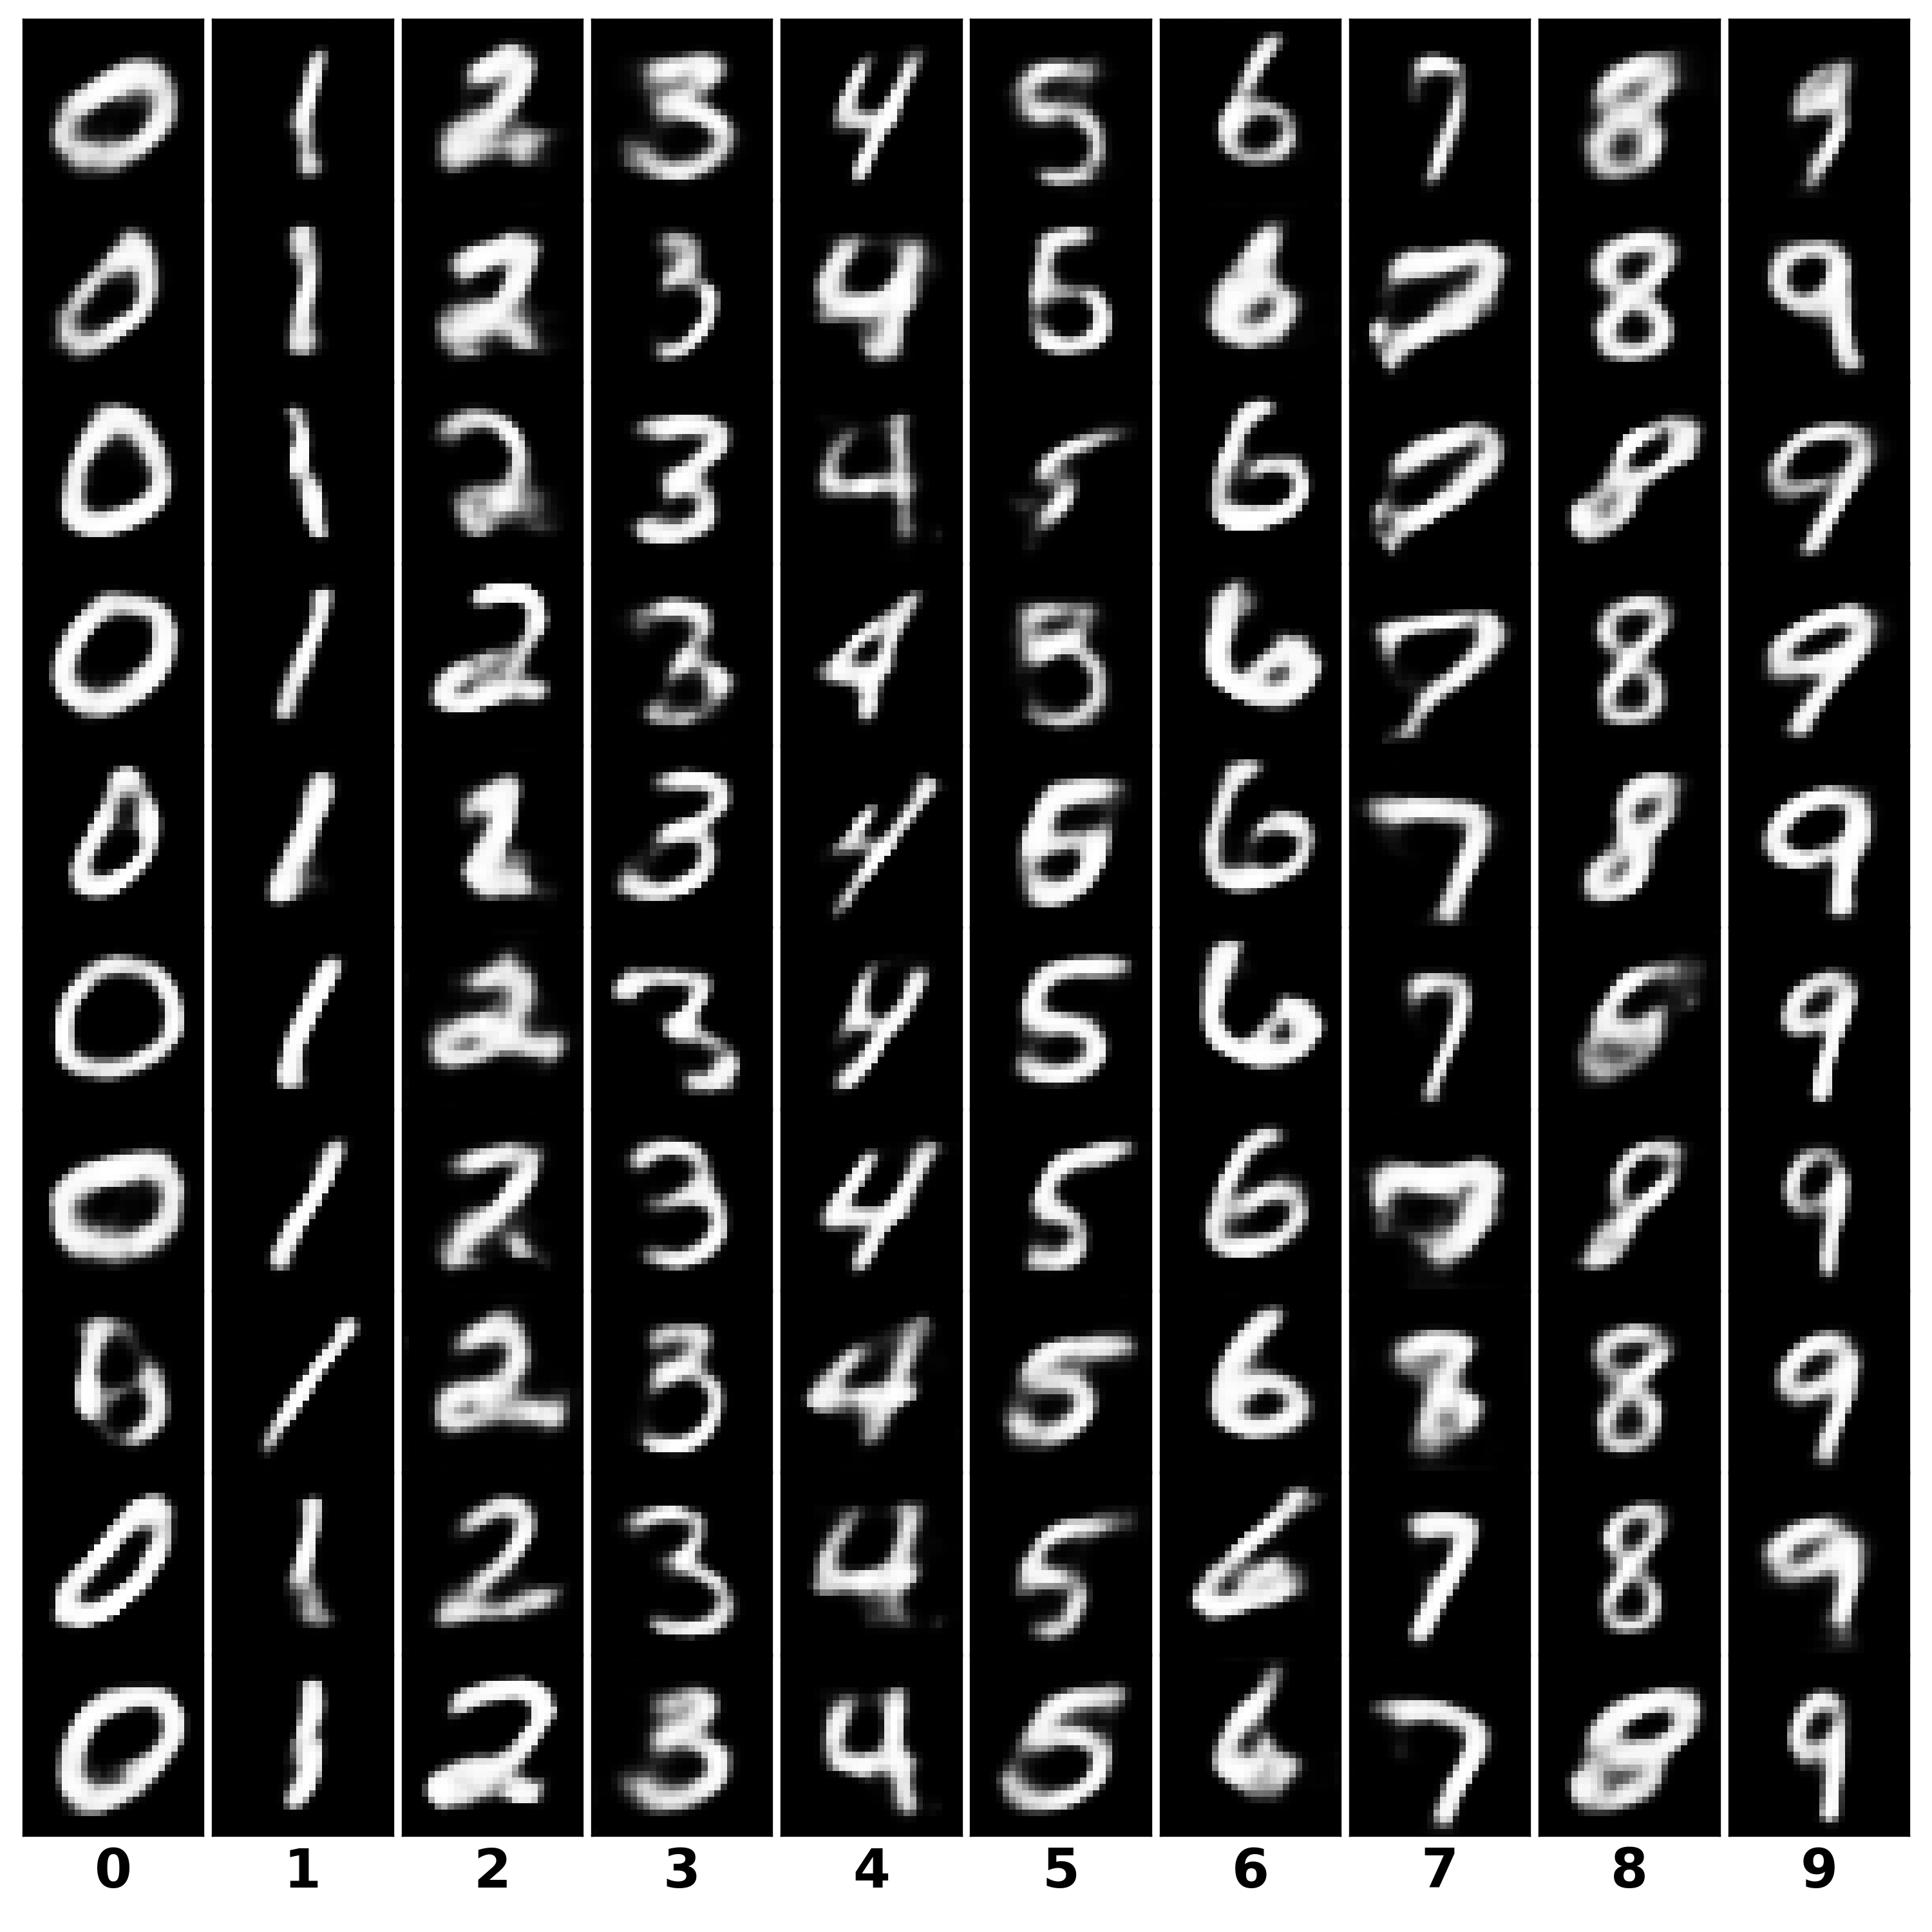
\includegraphics[width=0.7\textwidth]{Figures/Methods/IWRKM-congen-ubMNIST.png}
    \end{subfigure}
    \hfill
    \begin{subfigure}{0.45\textwidth}
        \centering
        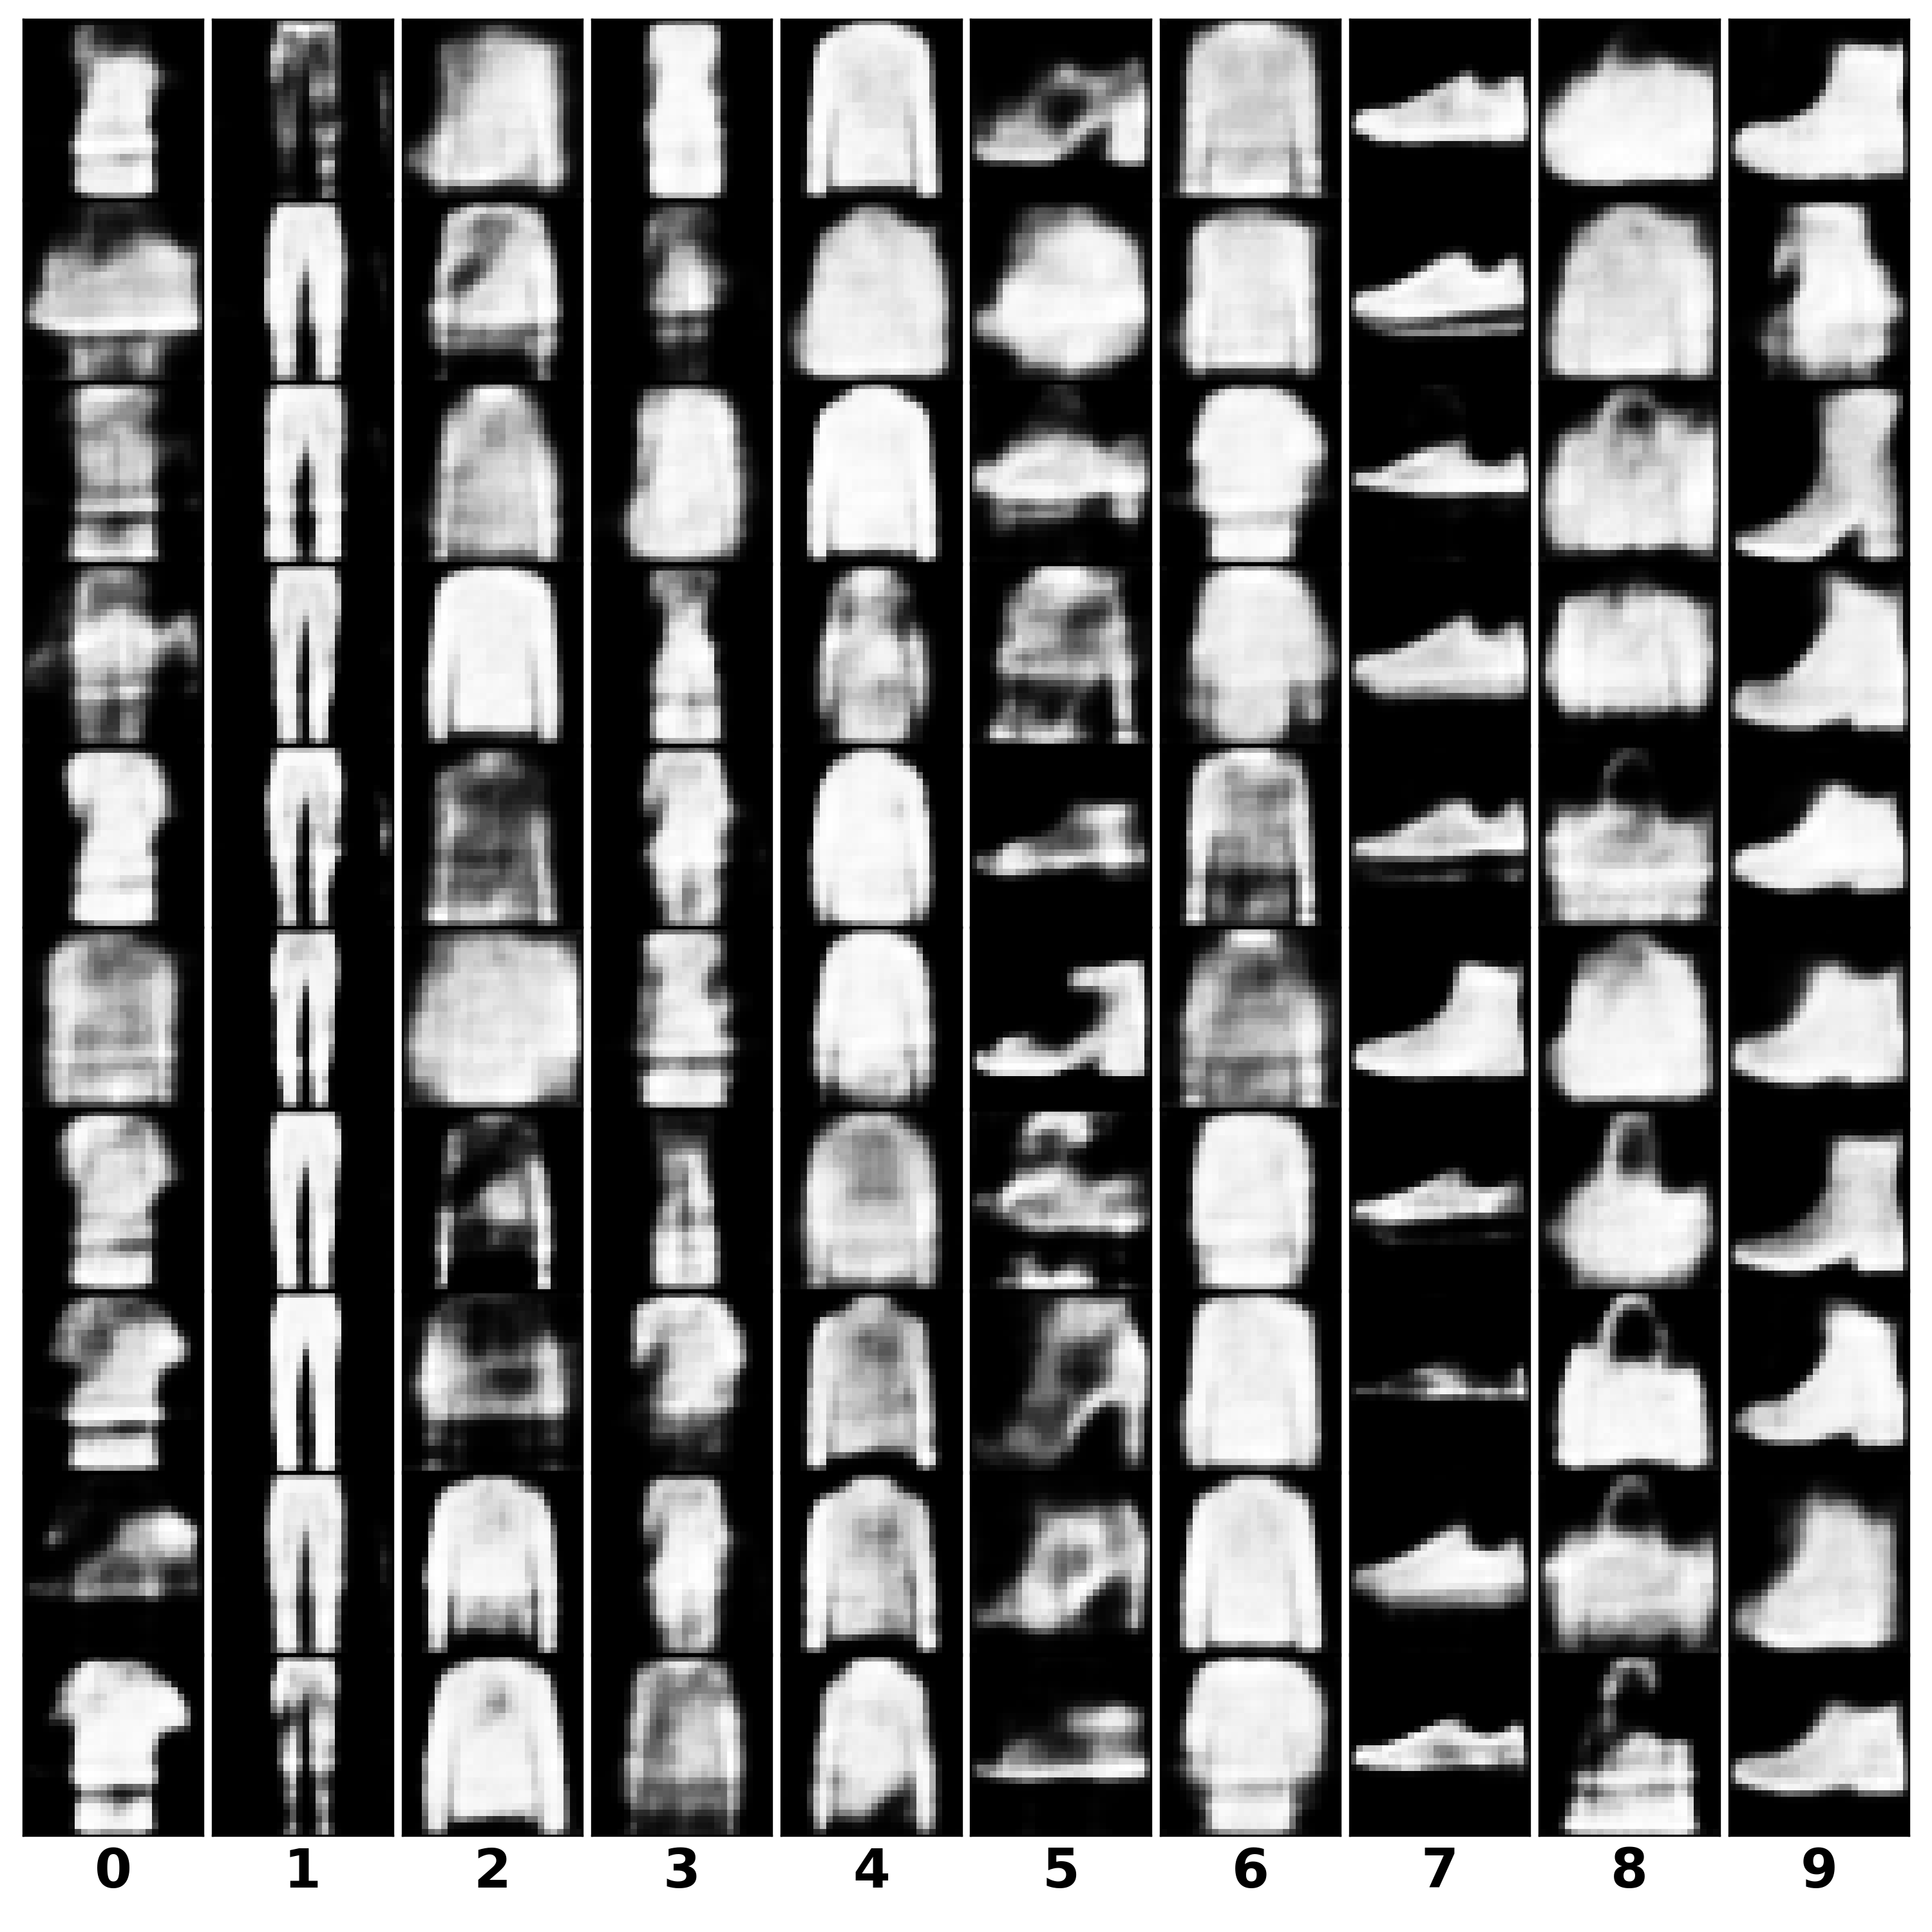
\includegraphics[width=0.7\textwidth]{Figures/Methods/RKM-congen-ubFashion.png}
    \end{subfigure}
    \hfill
    \begin{subfigure}{0.45\textwidth}
        \centering
        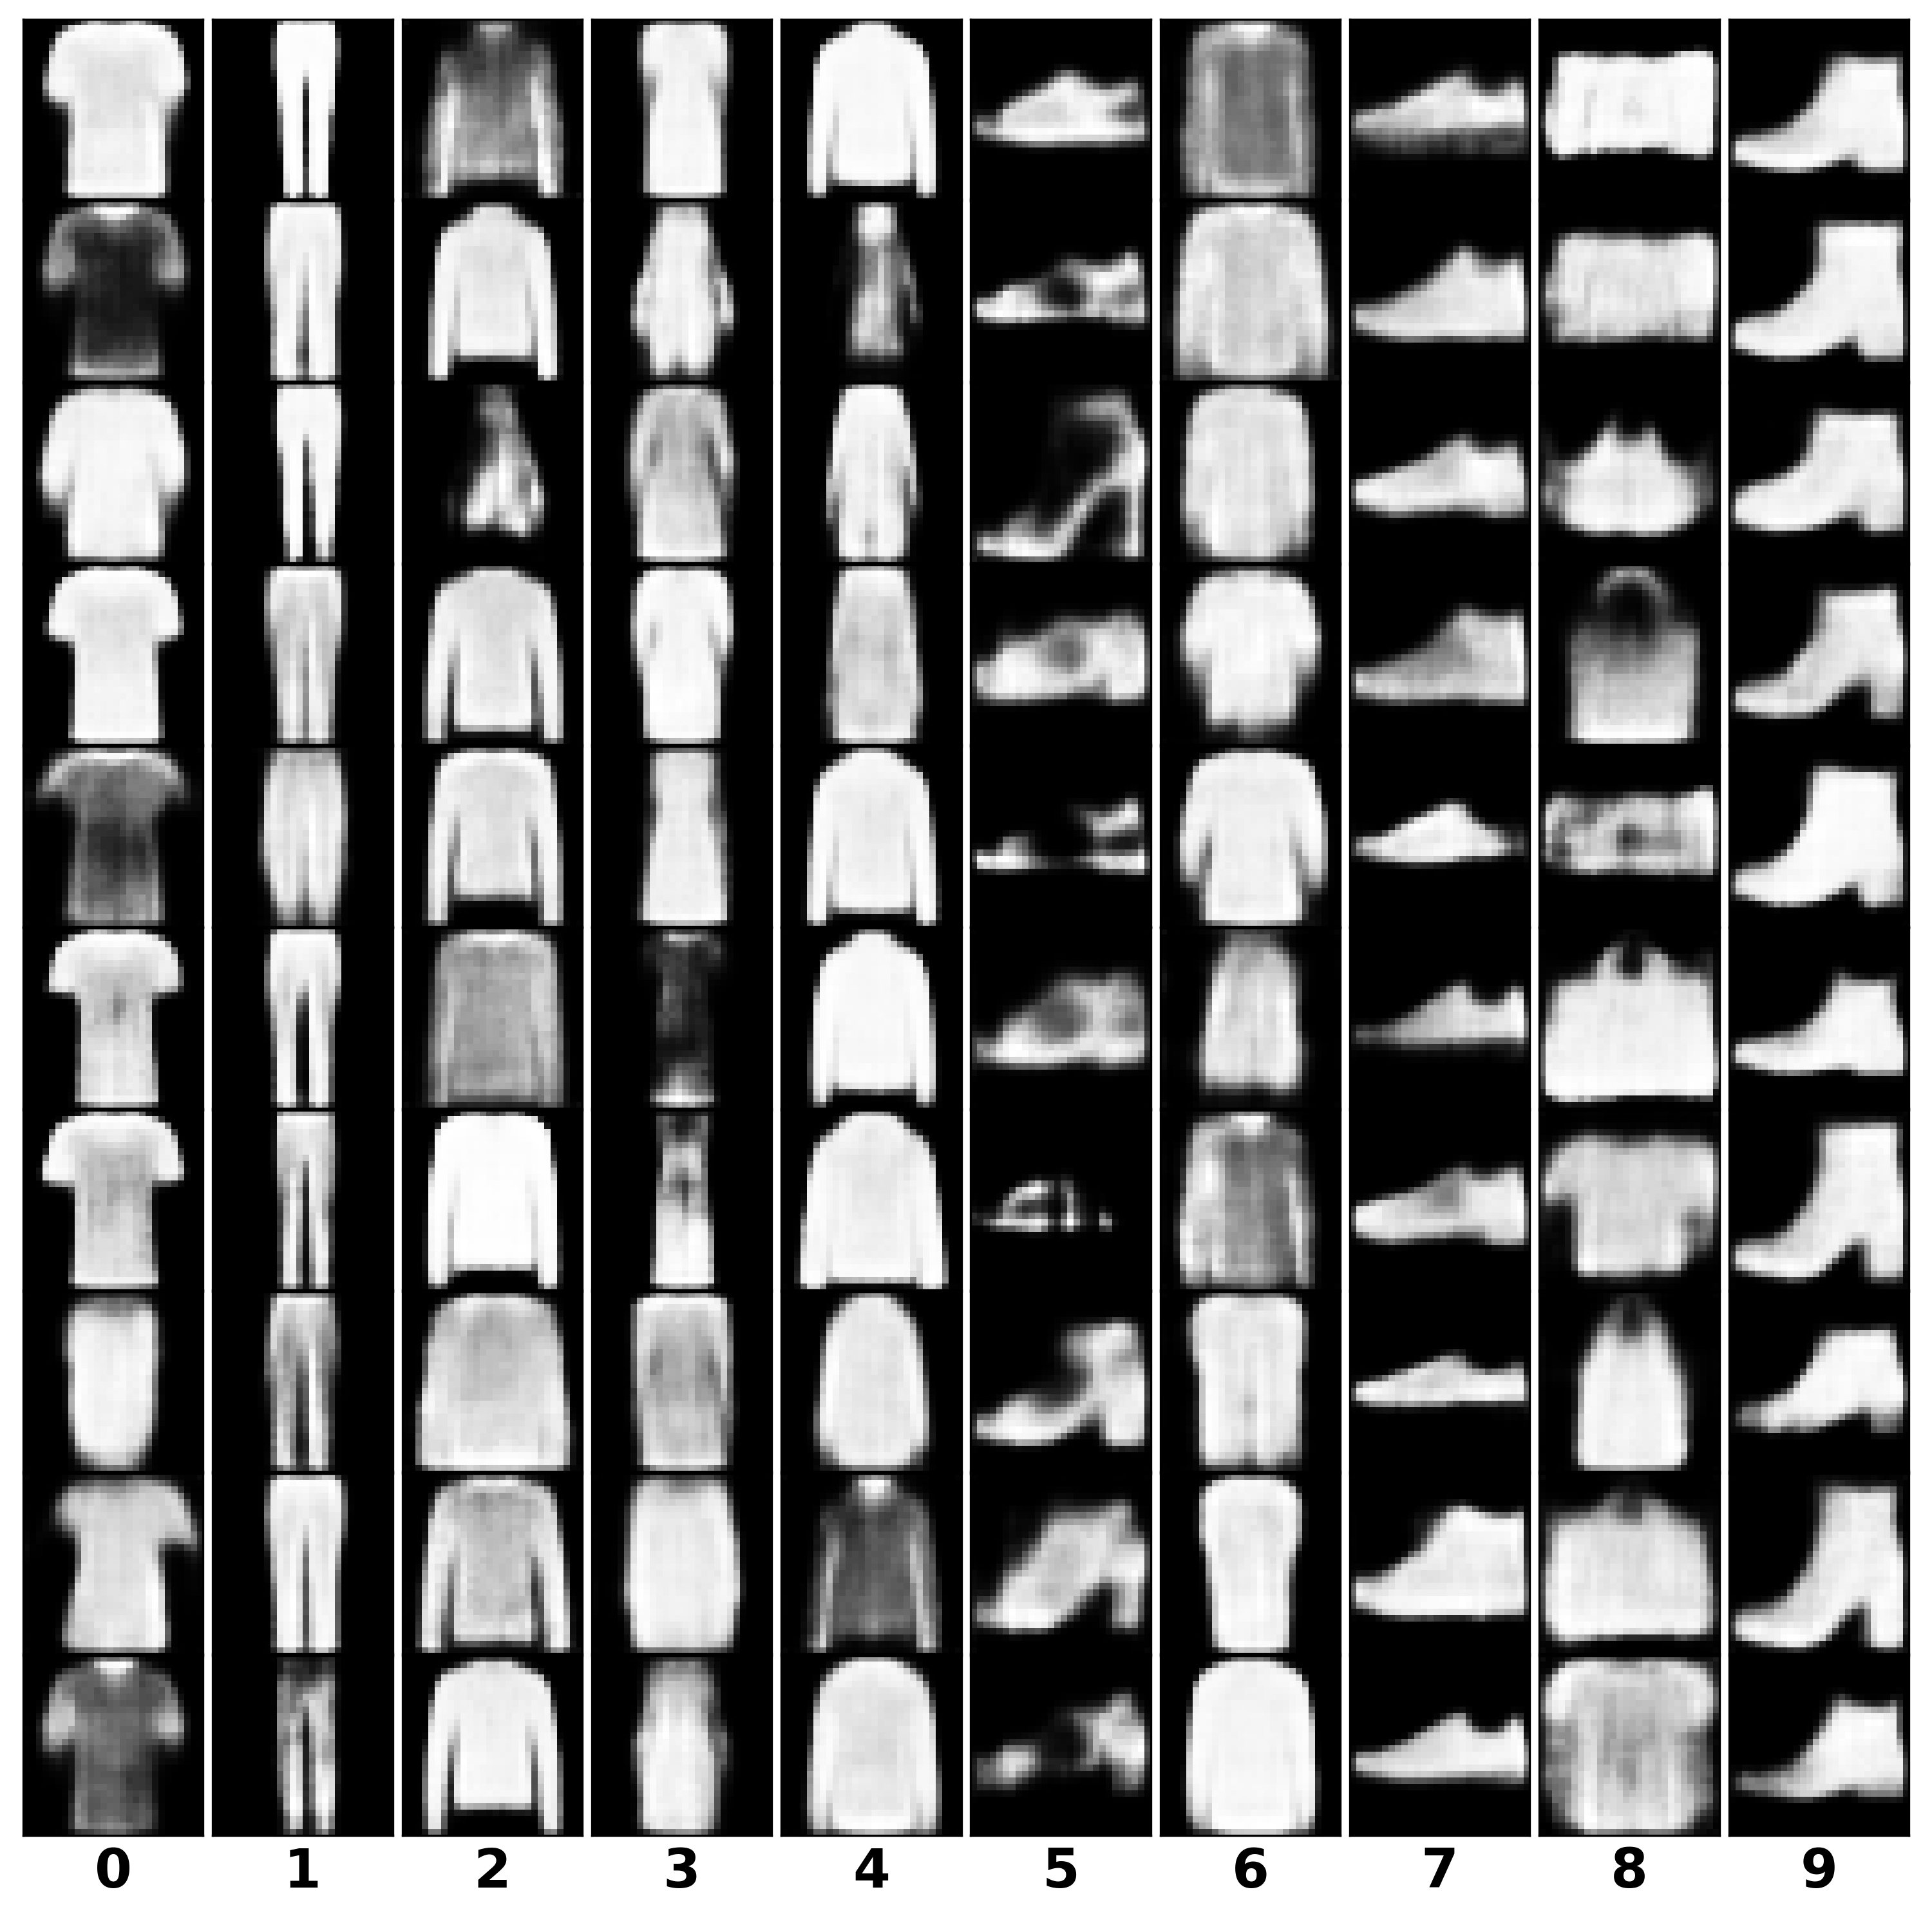
\includegraphics[width=0.7\textwidth]{Figures/Methods/IWRKM-congen-ubFashion.png}
    \end{subfigure}
    \caption{Conditional generations produced by multi-view Gen-RKM on the unbalanced MNIST dataset (top row) and the unbalanced Fashion MNIST dataset (bottom row). Figures in left column is generated by vanilla Gen-RKM, and figures in the right column are generated by Gen-RKM adapted with inverse frequency sampling. Images in each column of each figure are generated conditionally on a particular label. Imbalance ratios for both datasets are set to 0.1.}
    \label{fig-IWS-congen}
\end{figure}
\FloatBarrier

\section{Experiments on weighted sampling schemes under unsupervised setting}
\label{sec-expr-unsupervised}
In this section, we investigate the effectiveness of different diversity sampling schemes under unsupervised settings where no label information is provided during the training phase. Notice that label information is still required only for the purpose of evaluation. We start by evaluating RLS sampling in Gen-RKM on a toy 2D dataset in Section \ref{subsec-ringgrid}. Next, Section \ref{subsec-expr-ubMNIST012} and \ref{subsec-expr-ubMNIST} describe the results of experiments on MNIST-related datasets. In addition, results on Fashion MNIST under a similar setting are presented in Section \ref{subsec-expr-Fashion}. Lastly, some additional studies are conducted in \ref{subsec-additional-studies}.

\subsection{Synthetic ring/grid dataset}
\label{subsec-ringgrid}
The generated samples from models trained both with and without RLS sampling (using a shared feature map) are presented in Figure \ref{2d-rkm-vis}. It is evident from the visualization that the RKM, when trained using uniform sampling, fails to generate a sufficient number of points for the first four minority modes in the Ring and the first ten minority modes in the Grid. This problem is effectively solved by employing RLS sampling. The improved sampling effectiveness is demonstrated through the comparison of the two generation distributions for the Ring dataset, as shown in Figure \ref{fig-ring-rkm}. Meanwhile, Table \ref{tab-2d} presents the results of the two variants of RLS sampling, the primal form (shared feature map) and the dual form (RBF kernel with $\sigma=0.15$), on 2D synthetic datasets. Here, “minority mean” refers to the average number of points generated in each minority mode, while “number modes” indicates how many modes have generated more than 50 points. Both the primal and dual forms of RLS sampling enhance mode coverage and substantially increase the generation count in the minority modes.

\begin{figure}[ht]
    \centering
    \begin{subfigure}{0.32\textwidth}
        \centering
        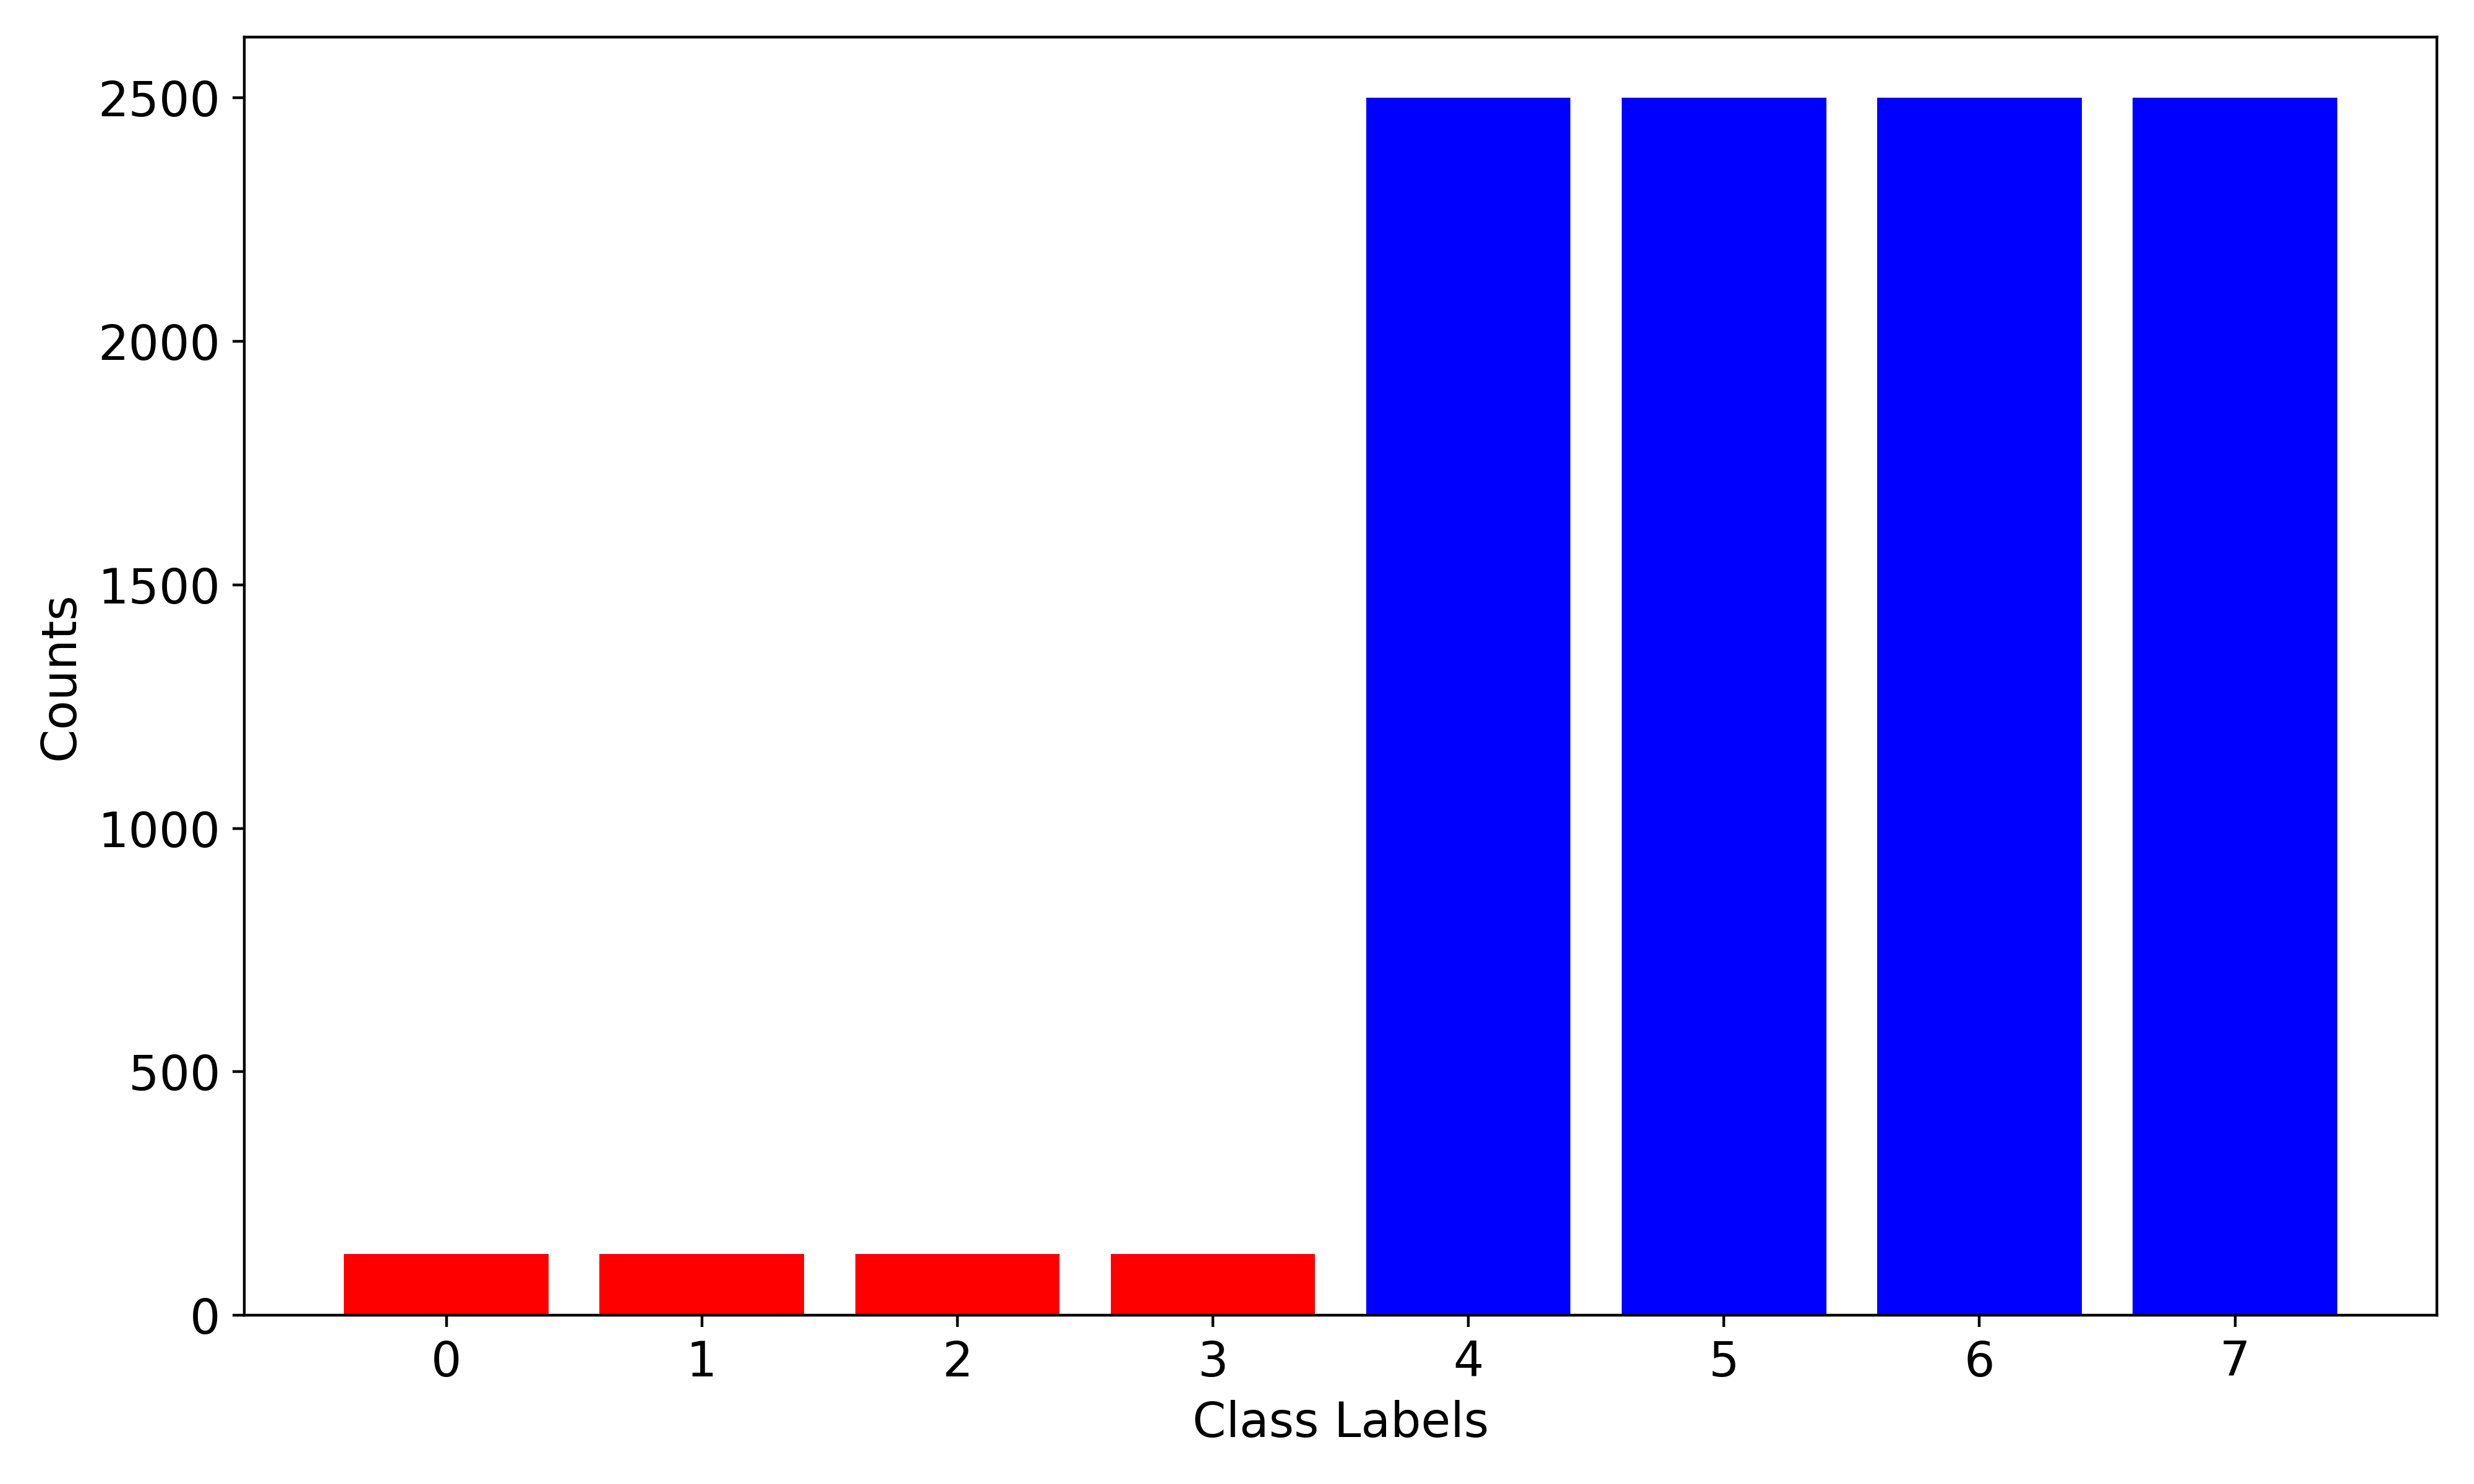
\includegraphics[width=0.9\textwidth]{Figures/Methods/ring_dis.png}
    \end{subfigure}
    %\hfill
    \begin{subfigure}{0.32\textwidth}
        \centering
        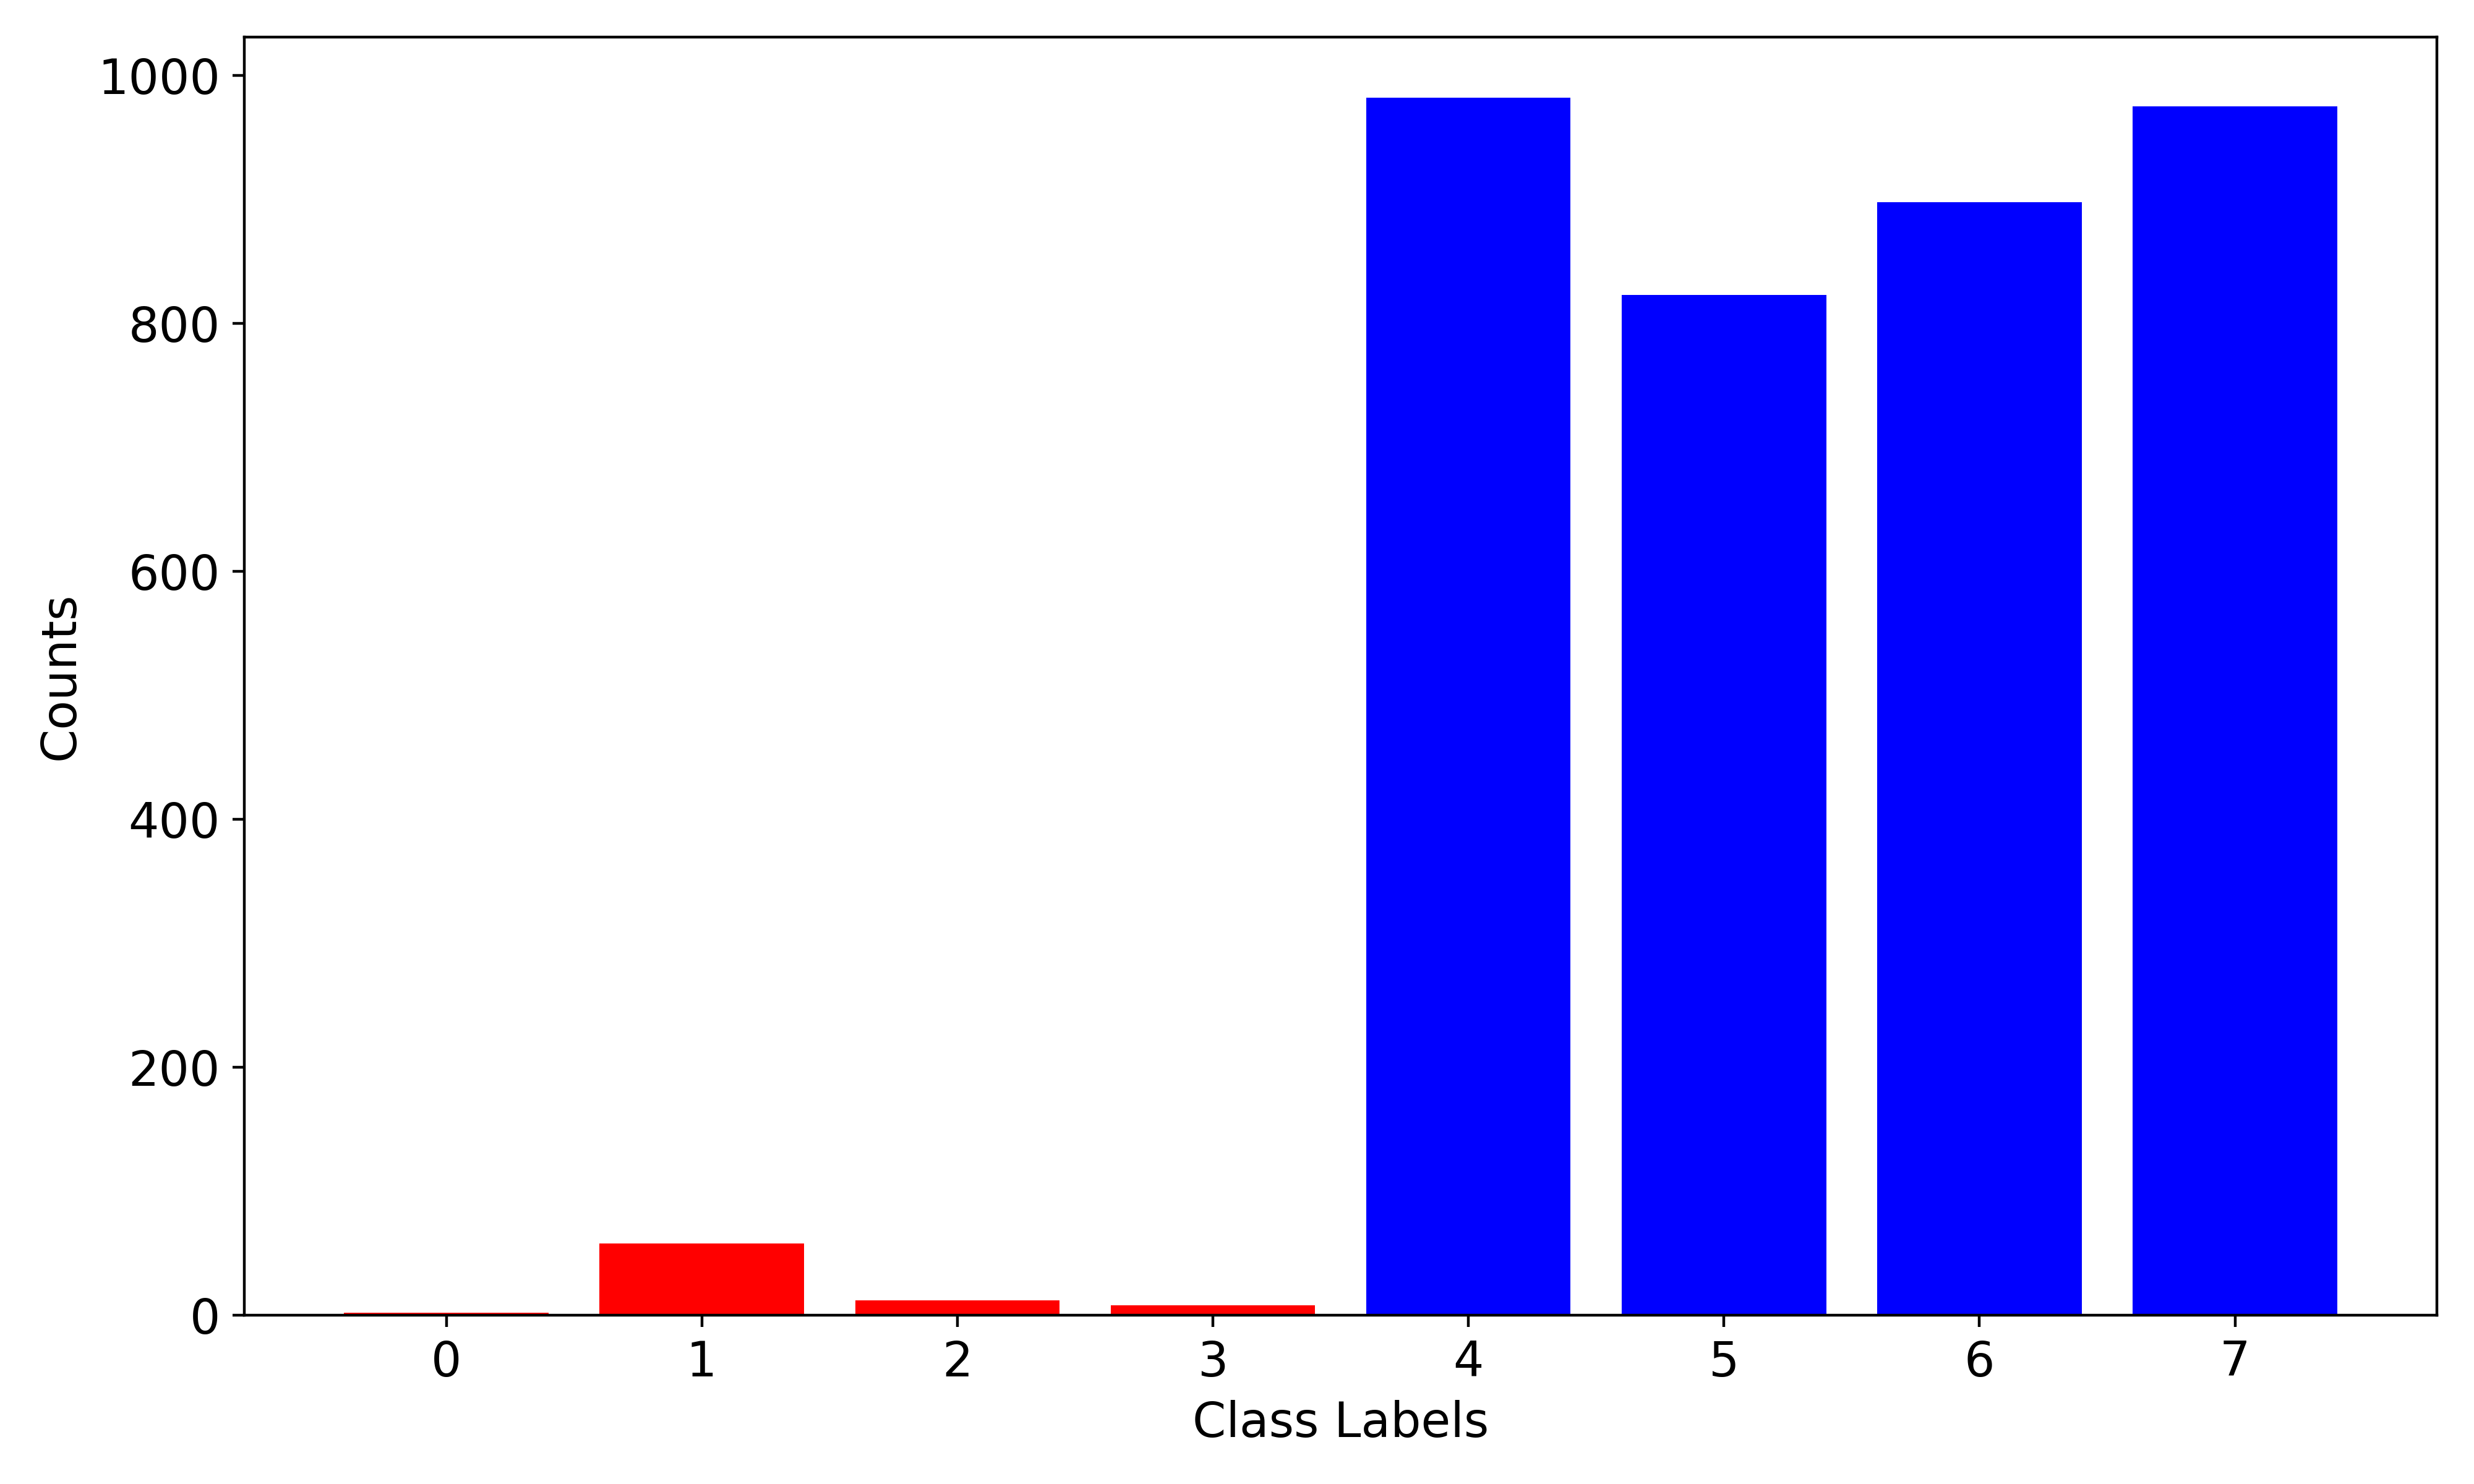
\includegraphics[width=0.9\textwidth]{Figures/Methods/ring_rkm.png}
    \end{subfigure}
    %\hfill
    \begin{subfigure}{0.32\textwidth}
        \centering
        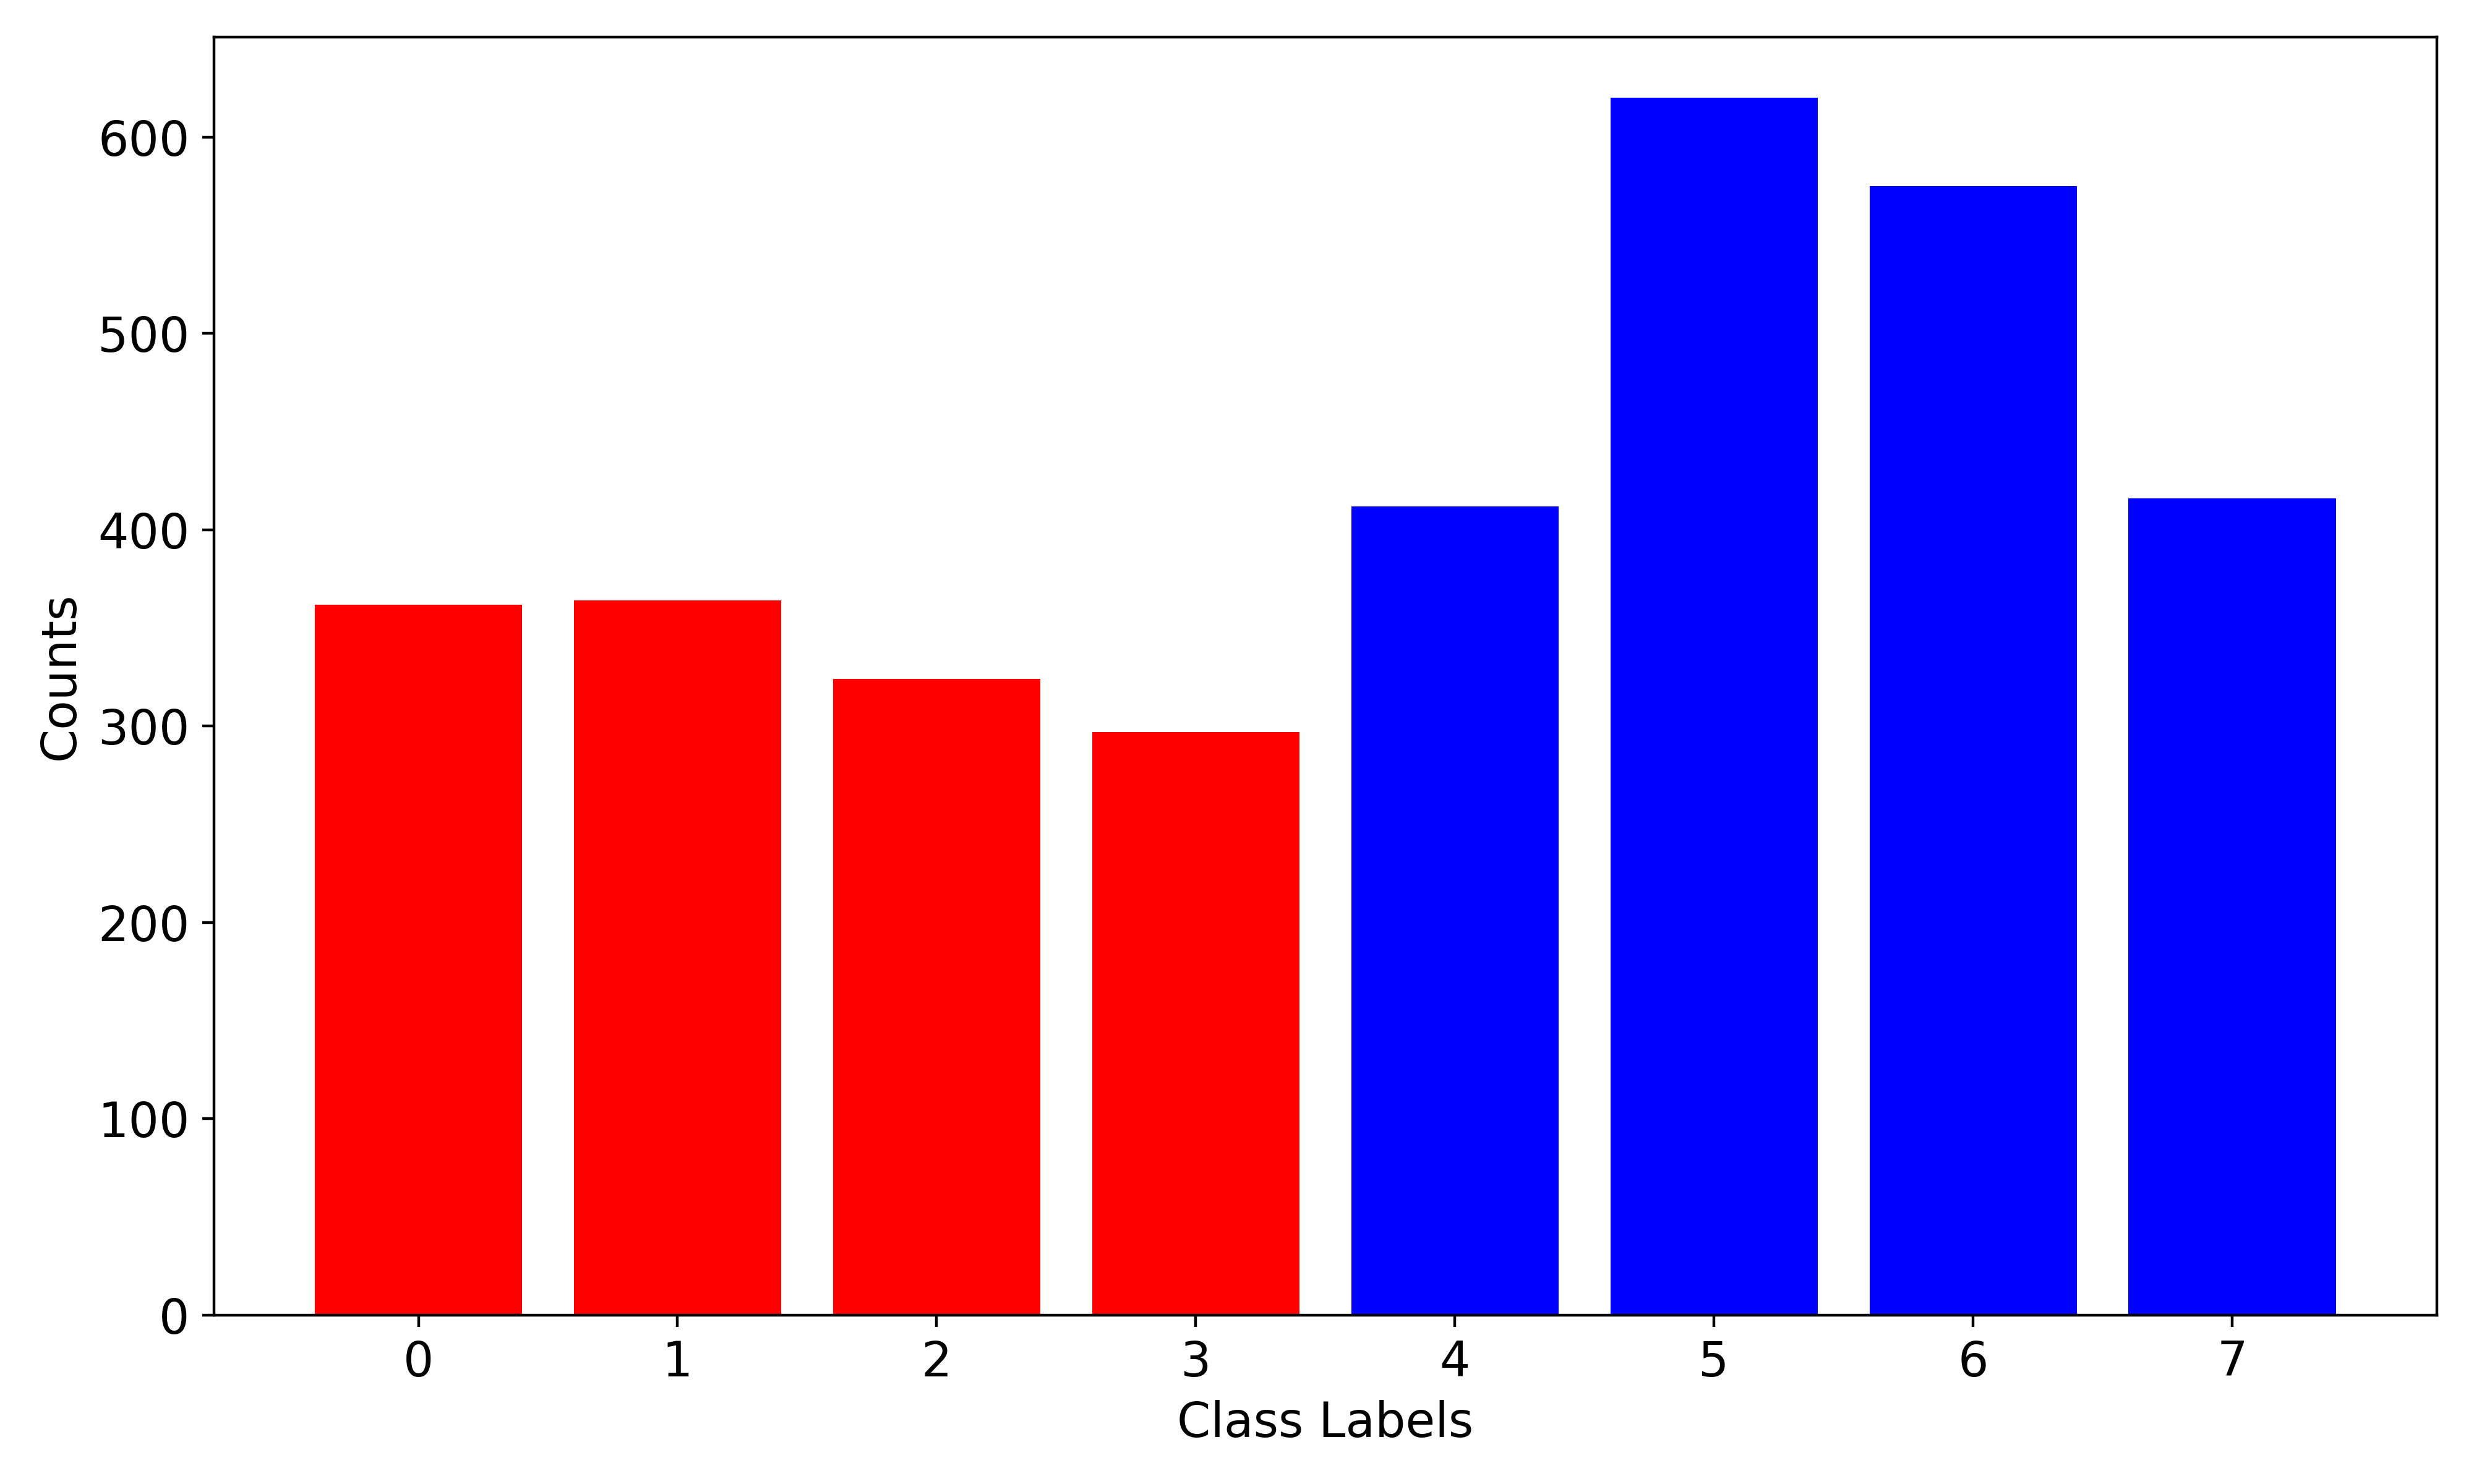
\includegraphics[width=0.9\textwidth]{Figures/Methods/ring_rls.png}
    \end{subfigure}
    \caption{Number of samples in each mode from RING dataset: Original RING(left), Vanilla Gen-RKM (middle) and Gen-RKM with RLS sampling (right).}
    \label{fig-ring-rkm}
\end{figure}

\begin{figure}[ht]
    \centering
    \begin{subfigure}{0.45\textwidth}
        \centering
        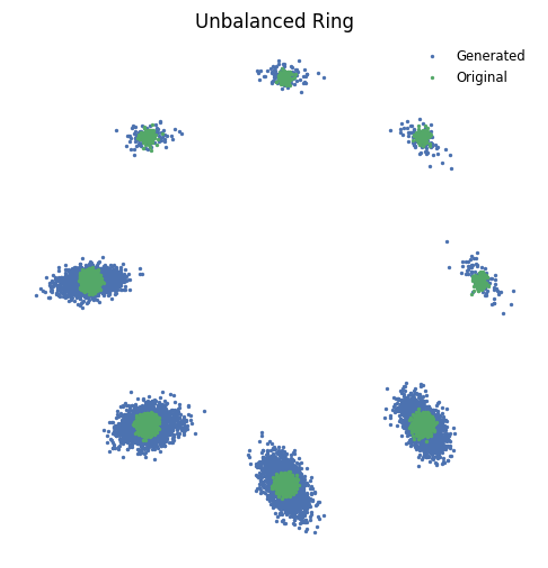
\includegraphics[width=0.8\textwidth]{Figures/Methods/2dring_rkm.png}
    \end{subfigure}
    \hfill
    \begin{subfigure}{0.45\textwidth}
        \centering
        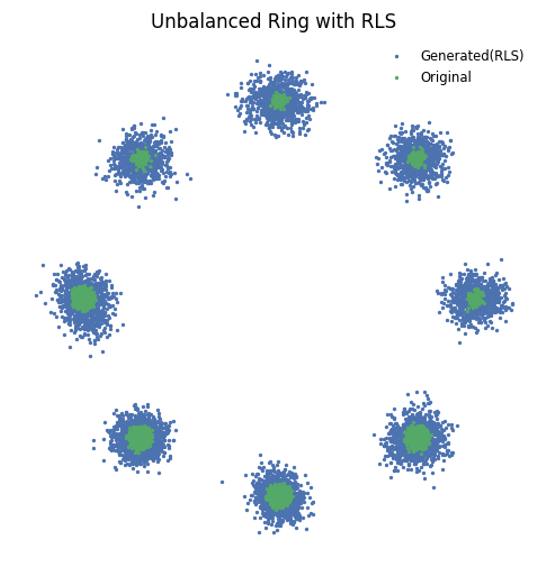
\includegraphics[width=0.8\textwidth]{Figures/Methods/2dring_rls.png}
    \end{subfigure}
    \hfill
    \begin{subfigure}{0.45\textwidth}
        \centering
        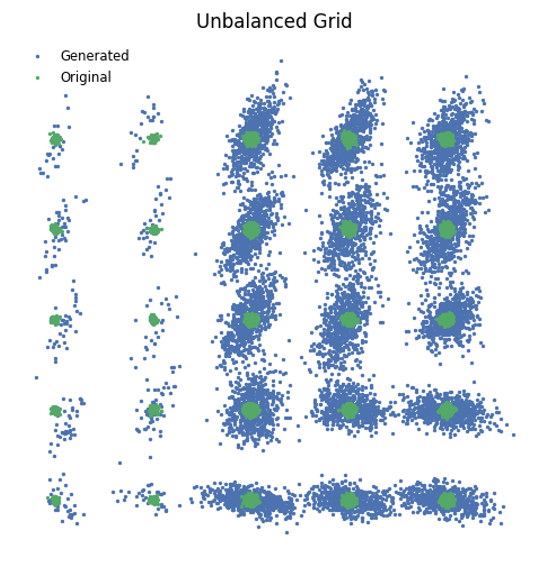
\includegraphics[width=0.8\textwidth]{Figures/Methods/2dgrid_rkm.png}
    \end{subfigure}
    \hfill
    \begin{subfigure}{0.45\textwidth}
        \centering
        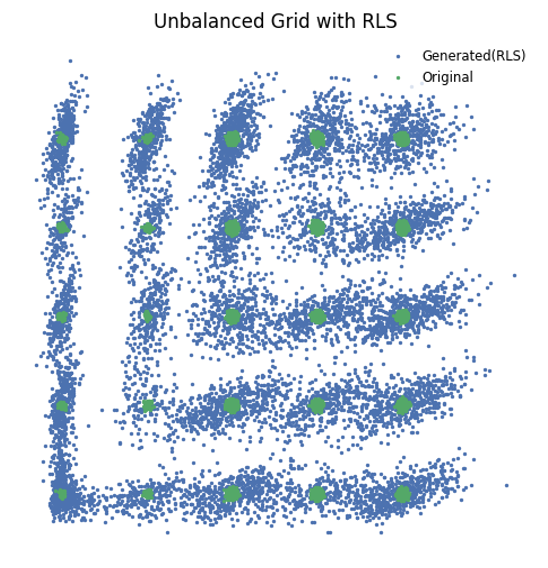
\includegraphics[width=0.8\textwidth]{Figures/Methods/2dgrid_rls.png}
    \end{subfigure}
    \caption{Visualizations of random generations on synthetic datasets: Vanilla Gen-RKM on RING (top left), Gen-RKM with RLS sampling on RING (top right), Vanilla Gen-RKM on GRID (down left) and Gen-RKM with RLS sampling on GRID (down right).}
    \label{2d-rkm-vis}
\end{figure}

\begin{table}[ht]
\centering
\begin{tabular}{@{}l*{4}{>{\centering\arraybackslash}p{2.5cm}}@{}}
\toprule
& \multicolumn{2}{c}{Ring with 8 modes} & \multicolumn{2}{c}{Grid with 25 modes} \\
\cmidrule(lr){2-3} \cmidrule(lr){4-5}
& Num modes & Minority mean & Num modes & Minority mean \\
\midrule
RKM      & 4.7(0.67) & 17.4(8.02) & 13.4(0.97) & 3.45(0.63) \\
RLS-RKM(shared)  & \textbf{7.7(0.48)} & 284.0(54.90) & 14.2(0.91) & \textbf{74.5(3.01)} \\
RLS-RKM(rbf) & 7.0(1.25) & \textbf{344.73(43.71)} & \textbf{20.02(1.75)} & 62.6(3.97) \\
\bottomrule
\end{tabular}
\caption{Results of experiments on 2D synthetic datasets (Experiments are replicated over 10 runs with random initialization).}
\label{tab-2d}
\end{table}


\FloatBarrier

\subsection{Unbalanced 012-MNIST}
\label{subsec-expr-ubMNIST012}
In this experiment, the performance of different weighted sampling schemes is studied on the unbalanced 012-MNIST dataset, which corresponds to a single minority mode scenario. Specifically, two RLS sampling variants with Gen-RKM are considered: RLSs computed based on an explicit feature map obtained from the last-to-next-layer of a pre-trained classifier (abbreviated as "RLS-RKM (class)"), and RLSs calculated from shared feature map with Gen-RKM (abbreviated as "RLS-RKM (shared)"), as described in Section \ref{subsec-methods-incor-rls-with-Genrkm}. In addition, weighted sampling built on isolation forest score (described in Section \ref{subsec-methods-islation-forest} and abbreviated as "Iforest RKM") is included. The baseline model in our experiment is Gen-RKM without any modifications but with the same network architecture and hyperparameter setting. In the evaluation process, the mode of each generated sample is identified by a well-trained MNIST classifier based on a ResNet18 architecture, which achieves 99.4\% accuracy on the test set. The results of calculated metrics are presented in Table \ref{expr-mnist012} where "Minority" refers to the number of generated samples classified as minority mode, and the distribution of numbers of generated samples under each mode is showcased in Figure \ref{fig-rls-gen-dist-ubmnist012}.  

It can be observed from Table \ref{expr-mnist012} that both RLS sampling and Iforest sampling could improve mode coverage and encourage more diverse generation under various imbalance ratio settings. More specifically, RLS-RKM (class) clearly outperforms all other methods in terms of both KL score and FID. Overall, This experiment demonstrates the immense effectiveness of RLS sampling with a pre-tained classifier as explicit feature map in single minority mode scenario. Samples from the minority group are generated more frequently as shown in Figure \ref{fig-gensamples-ubmnist012-rls}, thus a debiased generation is achieved.

\begin{table}[htb]
    \centering
    \begin{tabular}{ccccc}
\toprule
\makecell{Imbalance \\ ratio} & Model & Minority & KL score ($\downarrow$) & FID ($\downarrow$) \\
\midrule
\multirow{4}{*}{0.05} & RKM & 75 (±34) & 0.37 (±0.02) & 64.97 (±2.25) \\
& RLS-RKM (shared) & 410 (±60) & 0.32 (±0.02) & 74.09 (±3.39) \\
& RLS-RKM (class) & \textbf{1563} (±201) & \textbf{0.09} (±0.02) & \textbf{55.95} (±4.52) \\
& IforestRKM & 295 (±150) & 0.30 (±0.04) & 65.22 (±2.79) \\
\midrule
\multirow{4}{*}{0.10} & RKM & 135 (±76) & 0.35 (±0.03) & 65.04 (±1.74) \\
& RLS-RKM (shared) & 782 (±64) & 0.24 (±0.01) & 70.02 (±1.07) \\
& RLS-RKM (class) & \textbf{2259} (±144) & \textbf{0.03} (±0.01) & \textbf{55.42} (±6.33) \\
& IforestRKM & 863 (±180) & 0.18 (±0.03) & 59.63 (±3.74) \\
\midrule
\multirow{4}{*}{0.30} & RKM & 842 (±113) & 0.18 (±0.02) & 56.98 (±1.54) \\
& RLS-RKM (shared) & 2016 (±171) & 0.09 (±0.01) & 62.04 (±3.32) \\
& RLS-RKM (class) & \textbf{2868} (±77) & \textbf{0.01} (±0.00) & 51.95 (±3.60) \\
& IforestRKM & 2206 (±183) & 0.04 (±0.02) & \textbf{51.77} (±4.33) \\
\bottomrule
\end{tabular}
    \caption{Results of experiments on the unbalanced 012-MNIST dataset under different imbalance ratios. Experiments are replicated over 5 runs with random initializations. Means and standard deviations (enclosed in parentheses) for each metric are reported.}
    \label{expr-mnist012}
\end{table}
\begin{figure}[htb]
    \centering
    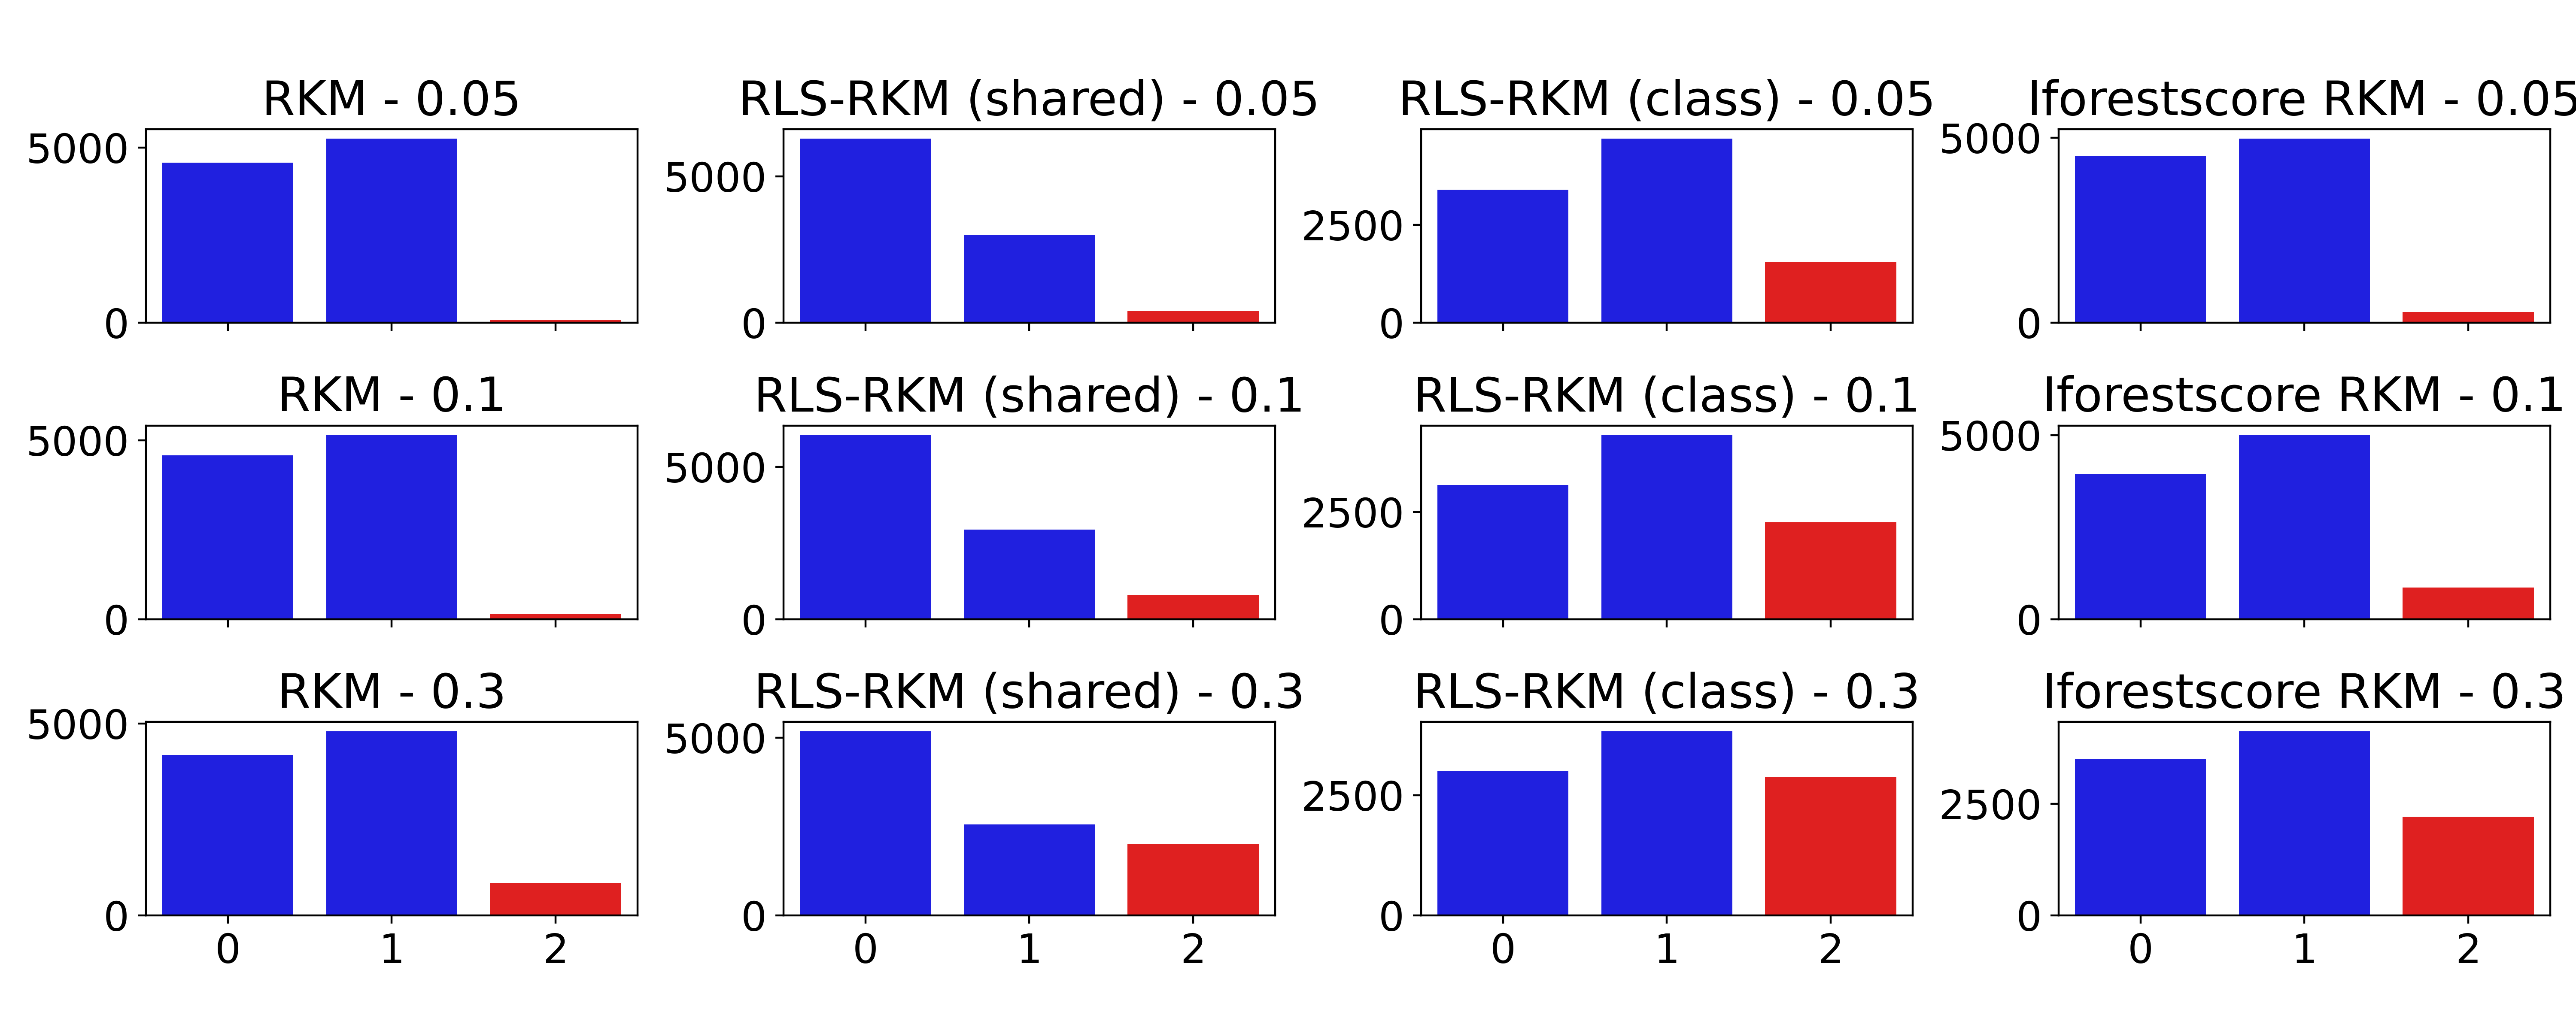
\includegraphics[width=0.9\linewidth]{Figures/Methods/expr-mnist012-gen-dist.png}
    \caption{Number of generated samples per mode from different RKM models on the unbalanced 012-MNIST dataset. Each row indicates that the dataset is generated with a specific balance ratio. Each column corresponds to a different model used. The minority mode in each figure is depicted in red color and, the majority modes are depicted in blue.}
    \label{fig-rls-gen-dist-ubmnist012}
\end{figure}

\subsection{Unbalanced MNIST}
\label{subsec-expr-ubMNIST}
It would also be meaningful to investigate how RLS sampling and Iforest sampling perform on a more challenging dataset, one that has multiple minority classes instead of just one. In the unbalanced MNIST dataset, half of the classes are minority classes, namely digits 0-4. Similarly, RLS-RKM (class) achieves best performance on KL score and FID compared with other approaches as observed from Table \ref{rls-expr-mnist}. Resampling schemes can more or less improve mode coverage in unbalanced data; however, when the imbalance ratio is very small (i.e., extremely unblanaced data), the improvement can be significantly diminished. If one looks at the distribution of generated labels in Figure \ref{fig-rls-gen-dist-ubmnist}, it is interesting to find that not all minority classes are oversampled when in RLS-RLM (class) and Iforest RKM. Instead, some particular minority classes might be downsampled. For example, minority classes such as digits 2,3, and 4 are generated even less frequently than before using RLS sampling or Iforest sampling, while only digits 0 and 1 are generated more frequently. This would ultimately result in a more unbalanced distribution of generated samples, as can be observed in the third and the fourth columns of Figure \ref{fig-rls-gen-dist-ubmnist}. Considering the sampling weights in both RLS (class) sampling and Iforest sampling are calculated based on embeddings extracted by a pre-trained classifier. Since this pre-trained classifier was not trained on this specific training dataset, it might fail to distinguish certain minority classes from others. The relatively low uniqueness results in a lower probability of being sampled. As for the RLS-RKM (shared), all minority classes are generally oversampled, but its ability to correct the imbalance is relatively weaker compared to other methods. To conclude, although weighted sampling schemes can more or less improve the diversity and quality of generation given unbalanced data with multiple minority modes, none of our methods could successfully captured all the underrepresented groups in the unbalanced MNIST dataset.
\begin{table}[ht]
    \centering
    \begin{tabular}{ccccc}
\toprule
\makecell{Imbalance \\ ratio} & Model & Minority mean & KL score ($\downarrow$) & FID ($\downarrow$) \\
\midrule
\multirow{4}{*}{0.05} & RKM & 113 (±13) & 0.49 (±0.02) & 39.19 (±1.17) \\
& RLS-RKM (shared) & 179 (±11) & 0.42 (±0.01) & 40.36 (±0.46) \\
& RLS-RKM (class) & \textbf{342} (±35) & \textbf{0.35} (±0.01) & \textbf{34.65} (±1.95) \\
& IforestRKM & 144 (±15) & 0.49 (±0.02) & 39.08 (±1.01) \\
\midrule
\multirow{4}{*}{0.10} & RKM & 185 (±11) & 0.40 (±0.01) & 38.89 (±0.18) \\
& RLS-RKM (shared) & 327 (±3) & \textbf{0.27} (±0.00) & 38.38 (±0.93) \\
& RLS-RKM (class) & \textbf{462} (±15) & \textbf{0.27} (±0.01) & \textbf{33.68} (±0.97) \\
& IforestRKM & 257 (±7) & 0.37 (±0.01) & 35.32 (±1.17) \\
\midrule
\multirow{4}{*}{0.30} & RKM & 478 (±14) & 0.15 (±0.01) & 34.09 (±1.28) \\
& RLS-RKM (shared) & 629 (±11) & \textbf{0.10} (±0.01) & 36.01 (±0.97) \\
& RLS-RKM (class) & \textbf{797} (±14) & 0.13 (±0.01) & \textbf{30.74} (±1.67) \\
& IforestRKM & 547 (±44) & 0.15 (±0.02) & 32.23 (±0.24) \\
\bottomrule
\end{tabular}
    \caption{Results of experiments on the unbalanced MNIST dataset under different imbalance ratios. Experiments are replicated over 3 runs with random initializations. Means and standard deviations (enclosed in parentheses) for each metric are reported. "Minority mean" refers to the average number of samples generated from each minority mode.
}
    \label{rls-expr-mnist}
\end{table}


\begin{figure}[ht]
    \centering
    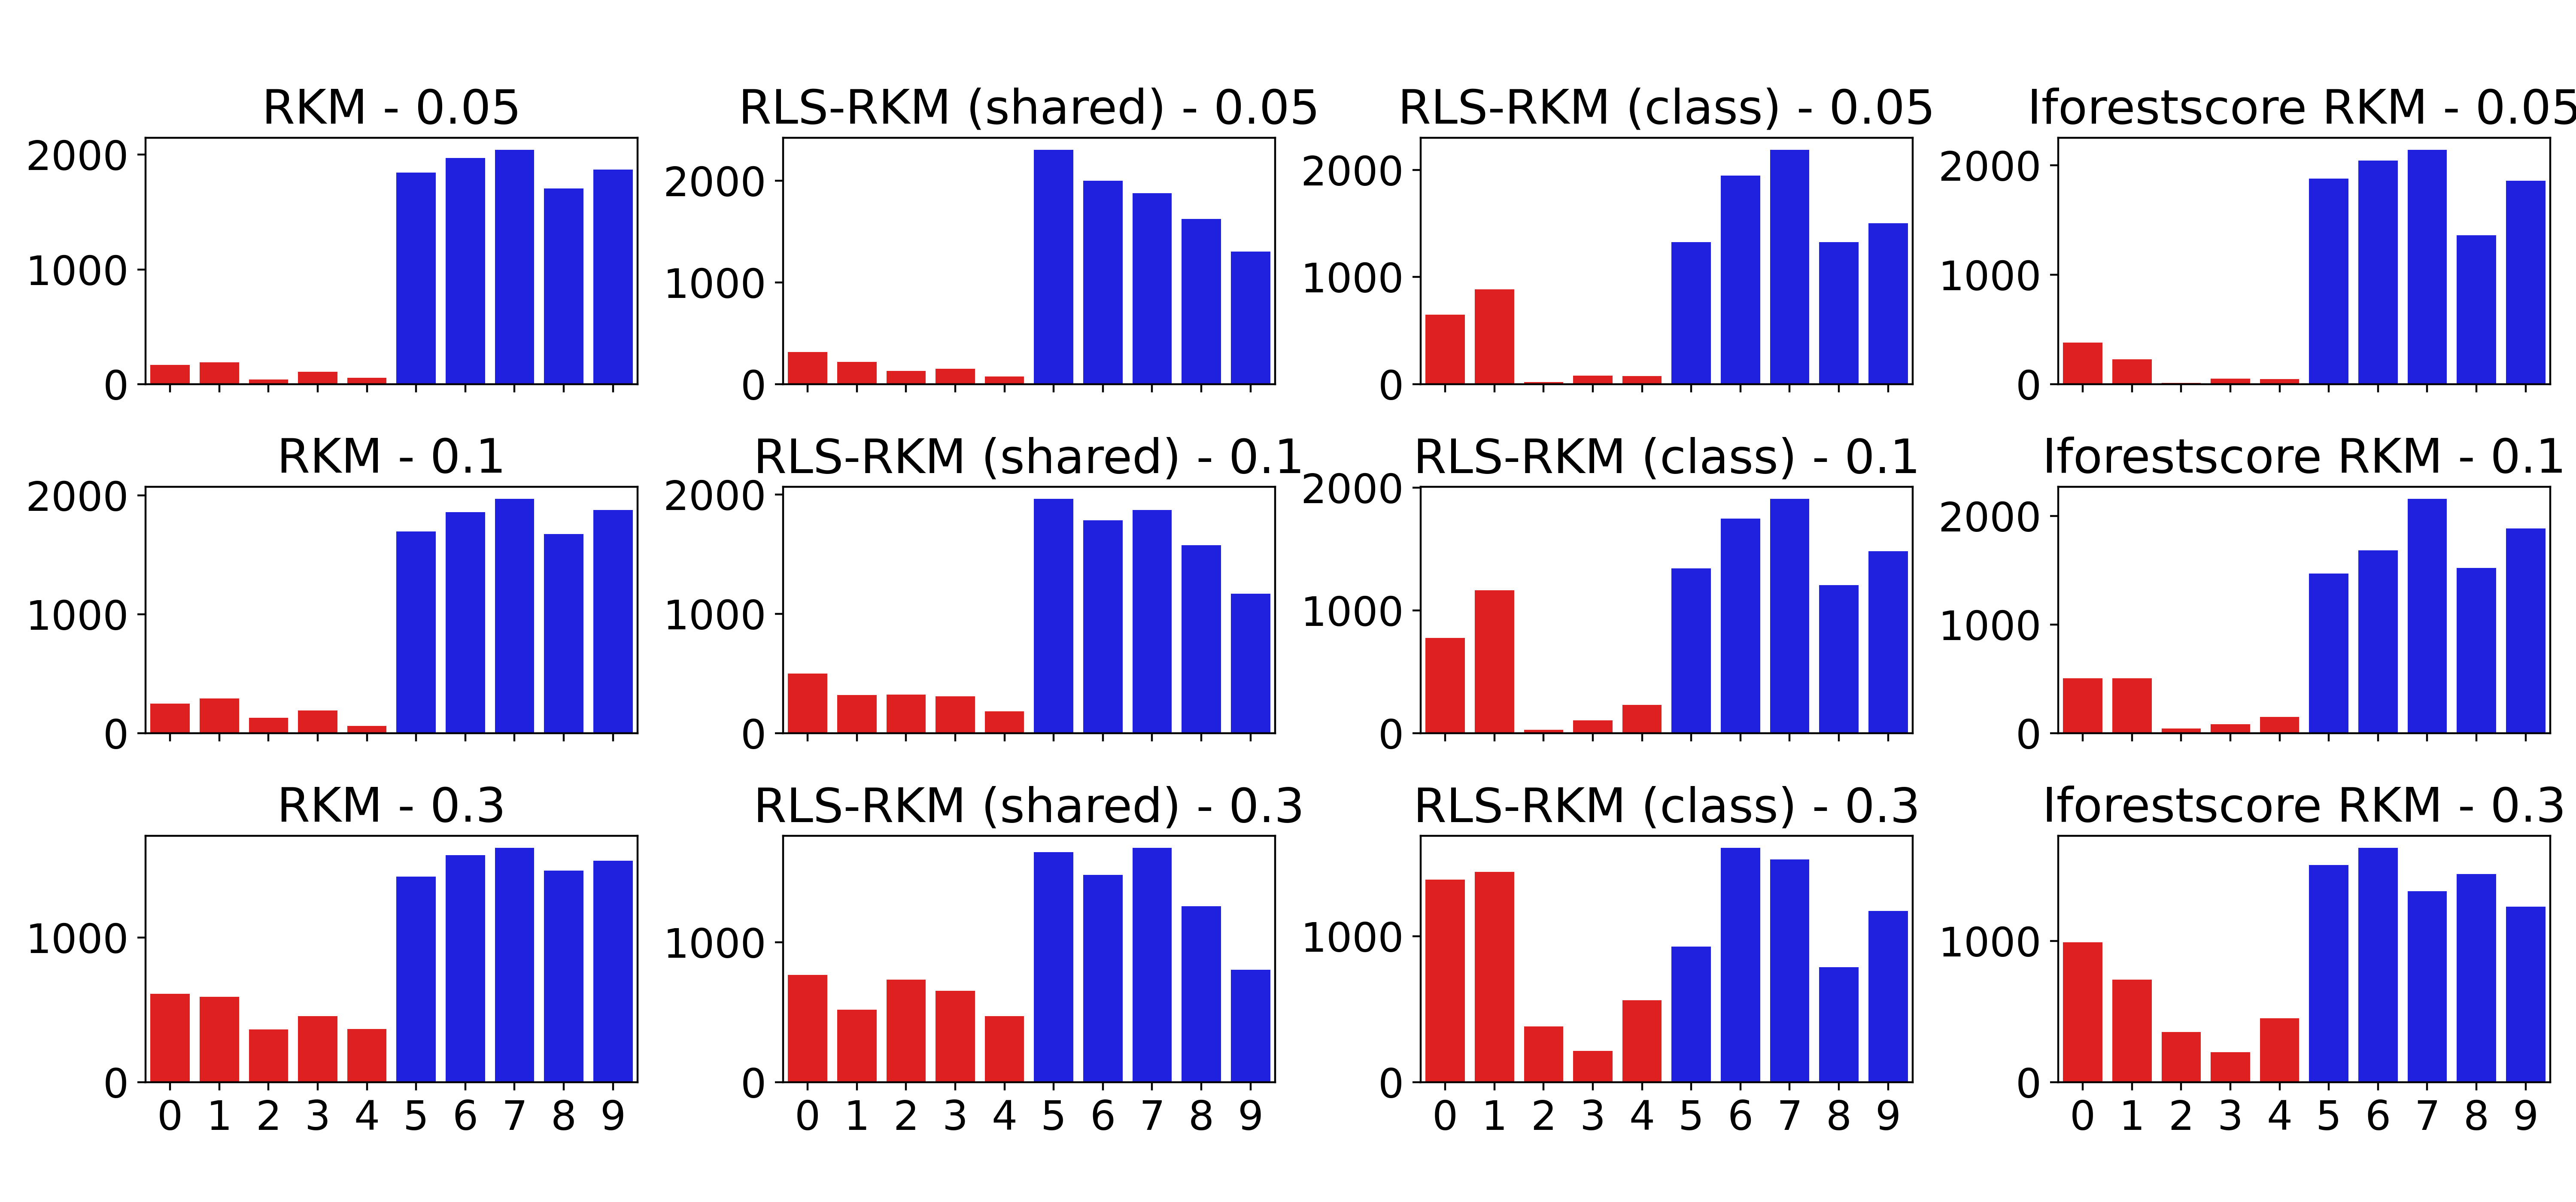
\includegraphics[width=0.9\linewidth]{Figures/Methods/expr-rls-mnist-gen-dist.png}
    \caption{Number of generated samples per mode from different RKM models on the unbalanced MNIST dataset.}
    \label{fig-rls-gen-dist-ubmnist}
\end{figure}


\subsection{Unbalanced Fashion MNIST}
\label{subsec-expr-Fashion}
Until now, experiments related to natural image datasets have only conducted on handwritten digits. In this section, we verify whether the use of RLS sampling and Iforest sampling in Gen-RKM could maintain similar performance on the Fashion MNIST dataset. The class of each generated sample is identified by a resnet18-type classifier which is trained up to 90.8\% accuracy on the test set. Unlike unbalanced MNIST, most of the categories in unbalanced Fashion MNIST are minority classes, whereas unbalanced MNIST has an equal number of minority and majority classes. The performance results of different sampling approaches are reported in Table \ref{tab-expr-fashion} and in Figure \ref{fig-rls-gen-dist-fashion}. Compared to the previous experiment, the performance of almost all methods is slightly better. Additionally, RLS-RKM (class) continues to outperform other methods, achieving the smallest FID and KL score on the unbalanced Fashion MNIST dataset.

\begin{table}[ht]
    \centering
    \begin{tabular}{ccccc}
\toprule
\makecell{Imbalance \\ ratio} & Model & Minority mean & KL score ($\downarrow$) & FID ($\downarrow$) \\
\midrule
\multirow{4}{*}{0.1} & RKM & 273 (±2) & 0.58 (±0.01) & 93.02 (±1.12) \\
& RLS-RKM (class) & \textbf{623} (±13) & \textbf{0.20} (±0.02) & \textbf{70.92} (±0.28) \\
& RLS-RKM (shared) & 437 (±2) & 0.38 (±0.02) & 80.98 (±2.35) \\
& Iforest RKM & 406 (±48) & 0.41 (±0.06) & 83.71 (±4.15) \\
\bottomrule
\end{tabular}
    \caption{Results of experiments on unbalanced Fashion MNIST dataset. Experiments are replicated over 3 runs with random initializations. Means and standard deviations (enclosed in parentheses) for each metric are reported. "Minority mean" refers to the average number of samples generated from each minority mode.}
    \label{tab-expr-fashion}
\end{table}
\begin{figure}[ht]
    \centering
    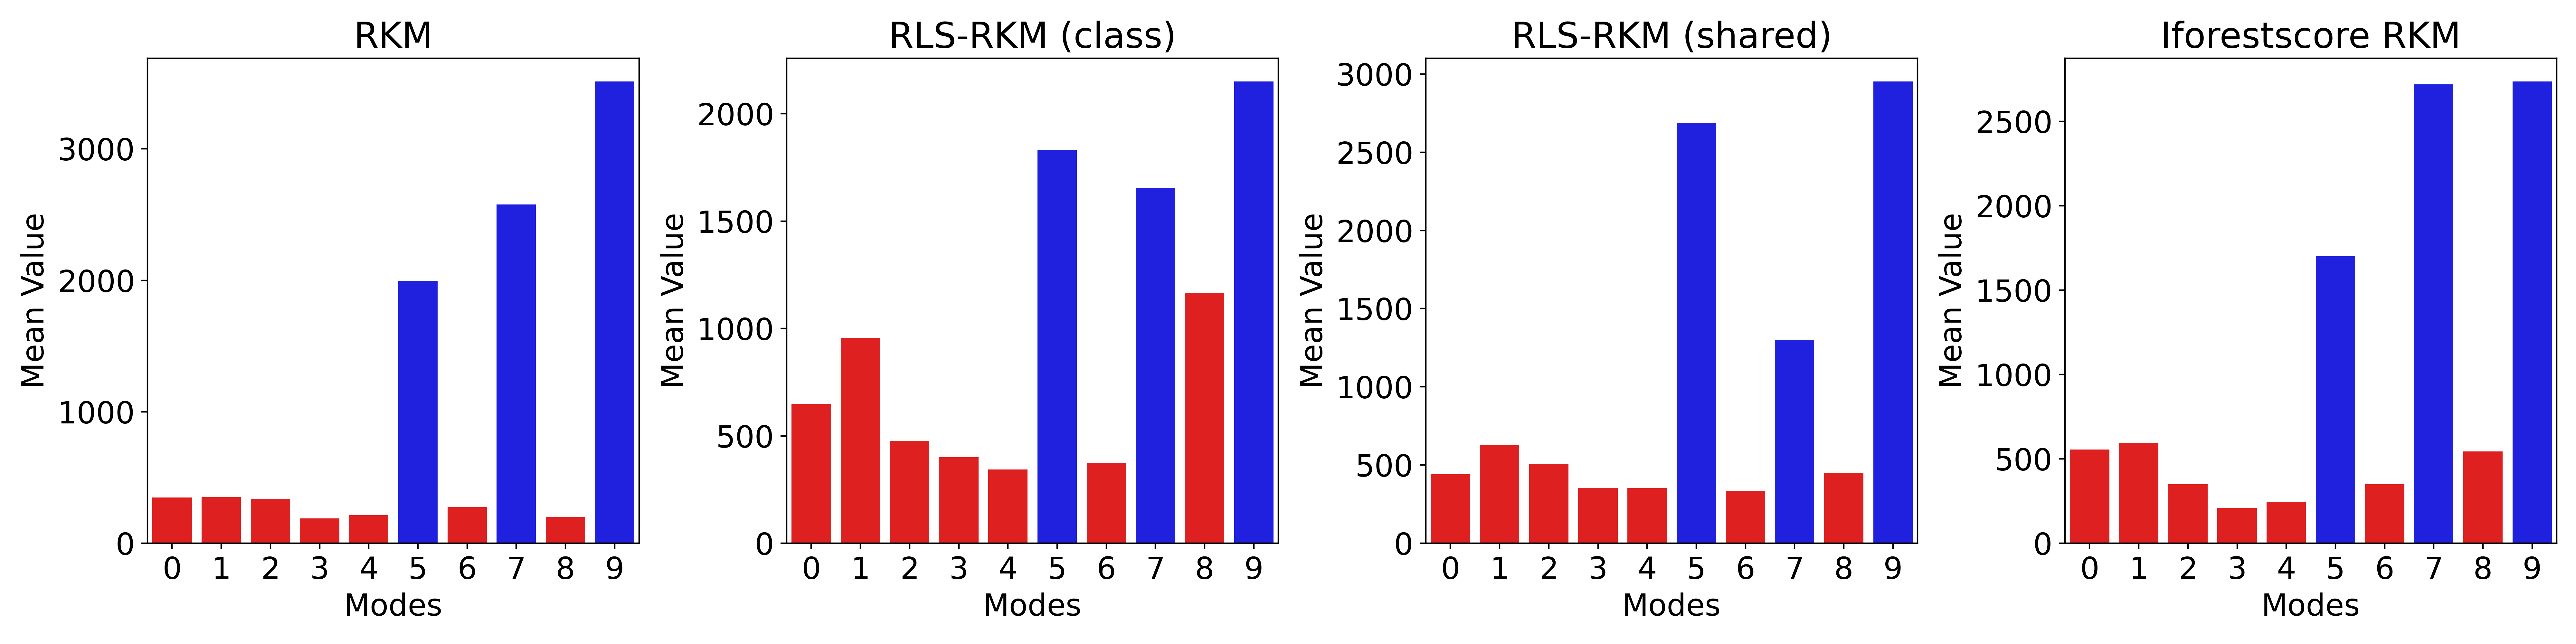
\includegraphics[width=0.9\linewidth]{Figures/Methods/expr-rls-fashion-gen-dist.png}
    \caption{Number of generated samples per mode from different RKM models on the unbalanced Fashion MNIST dataset.}
    \label{fig-rls-gen-dist-fashion}
\end{figure}

\subsection{Additional studies}
\label{subsec-additional-studies}

\begin{description}[leftmargin=0pt]
    \item[Ablation study on different pre-trained classifiers ] In the original work of RLS-GAN \cite{schreursLeverageScoreSampling2022}, the fixed explicit feature map for computing RLSs is derived from the last-to-the-next layer of an Inception-v3 network. However, the impact of different pre-trained classifiers was not compared. In this Section, an ablation study over the impact of various pre-trained classifiers in RLS-RKM (class) on the unbalanced 012-MNIST dataset is conducted. Specifically, the candidate pre-trained classifiers considered in our experiment include ResNet18\cite{heDeepResidualLearning2016}, ResNet34\cite{heDeepResidualLearning2016}, VGG16\cite{simonyanVeryDeepConvolutional2015}, AlexNet\cite{krizhevskyImageNetClassificationDeep2012}, and Inception-v3\cite{szegedyRethinkingInceptionArchitecture2016}. As shown in Table \ref{expr-different-classifiers}, we empirically observe that RLS sampling with pre-trained AlexNet as explicit feature map achieves the best performance across all evaluation metrics.

    \begin{table}[ht]
\centering
\begin{tabular}{lccccc}
\toprule
                     Classifier &      Mode 1 &      Mode 2 &      \textbf{Mode 3} &       KL score($\downarrow$) &           FID($\downarrow$) \\
\midrule
     Alexnet\cite{krizhevskyImageNetClassificationDeep2012} & 3219 (±218) & 4183 (±125) & \textbf{2283} (±299) & \textbf{0.03} (±0.02) & \textbf{52.02} (±4.32) \\
Inception\_v3\cite{szegedyRethinkingInceptionArchitecture2016} & 3998 (±242) & 4496 (±122) & 1206 (±278) & 0.12 (±0.04) &   60.4 (±4.4) \\
    Resnet18\cite{heDeepResidualLearning2016} & 3706 (±188) &  4231 (±94) & 1738 (±286) & 0.06 (±0.02) &  57.31 (±3.7) \\
    Resnet34\cite{heDeepResidualLearning2016} &  3328 (±59) & 4945 (±177) & 1486 (±231) &  0.1 (±0.02) &  55.34 (±3.0) \\
       vgg16\cite{simonyanVeryDeepConvolutional2015} &  3765 (±77) & 4538 (±183) & 1446 (±130) & 0.09 (±0.02) & 59.53 (±2.11) \\
\bottomrule
\end{tabular}
\caption{Ablation study over the impact of different pre-trained classifiers on the performance of RLS-RKM (class) on the unbalanced 012-MNIST dataset. Minority mode is highlighted in bold, with the imbalance ratio set to 0.1. The results are averaged over 5 runs of replicated experiments.}
\label{expr-different-classifiers}
\end{table}

    \item[Effect of weighted sampling on latent space in Gen-RKM ] It is also non-trivial to analyze the impact of the use of weighted sampling schemes during training in Gen-RKM on its corresponding latent space. The visualizations of the latent spaces obtained from the standard training process and that from the RLS sampling-adapted training process are shown in Figure \ref{fig-rls-latent-space-vis}. It is evident that the latent variables corresponding to the minority classes are also augmented in the latent space, and a re-balancing effect is significant. This ensures that the fitted GMM would not overlook these underrepresented groups, thereby reducing the unwanted bias towards majority modes that arise from unbalanced training data in generation. A more diverse and fair generation can thus be obtained in this spirit.

    \indent However, augmenting minority classes via oversampling techniques also has some drawbacks. Since correction for imbalance is achieved by oversampling the minority classes, the resampled training data will inevitably contain some duplicate instances. During the KPCA operation, these duplicate data will still yield redundant hidden representations in the latent space, as displayed in the right side of Figure \ref{fig-rls-latent-space-vis}. The negative effects are in two-fold. First, the smoothness and the continuity of the latent space are no longer guaranteed, where interpolation between latent points could be problematic. Second, the presence of duplicate latent points might cause the GMM to be overfitted, where duplicate points are assigned higher probabilities. That would increase the risk of data-copying (i.e., directly replicating certain training samples in generation) in the generative models, which has been shown as orthogonal to the problem of mode collapse \cite{bhattacharjeeDatacopyingGenerativeModels2023}.  

    \begin{figure}[ht]
    \centering
    \begin{subfigure}{0.45\textwidth}
        \centering
        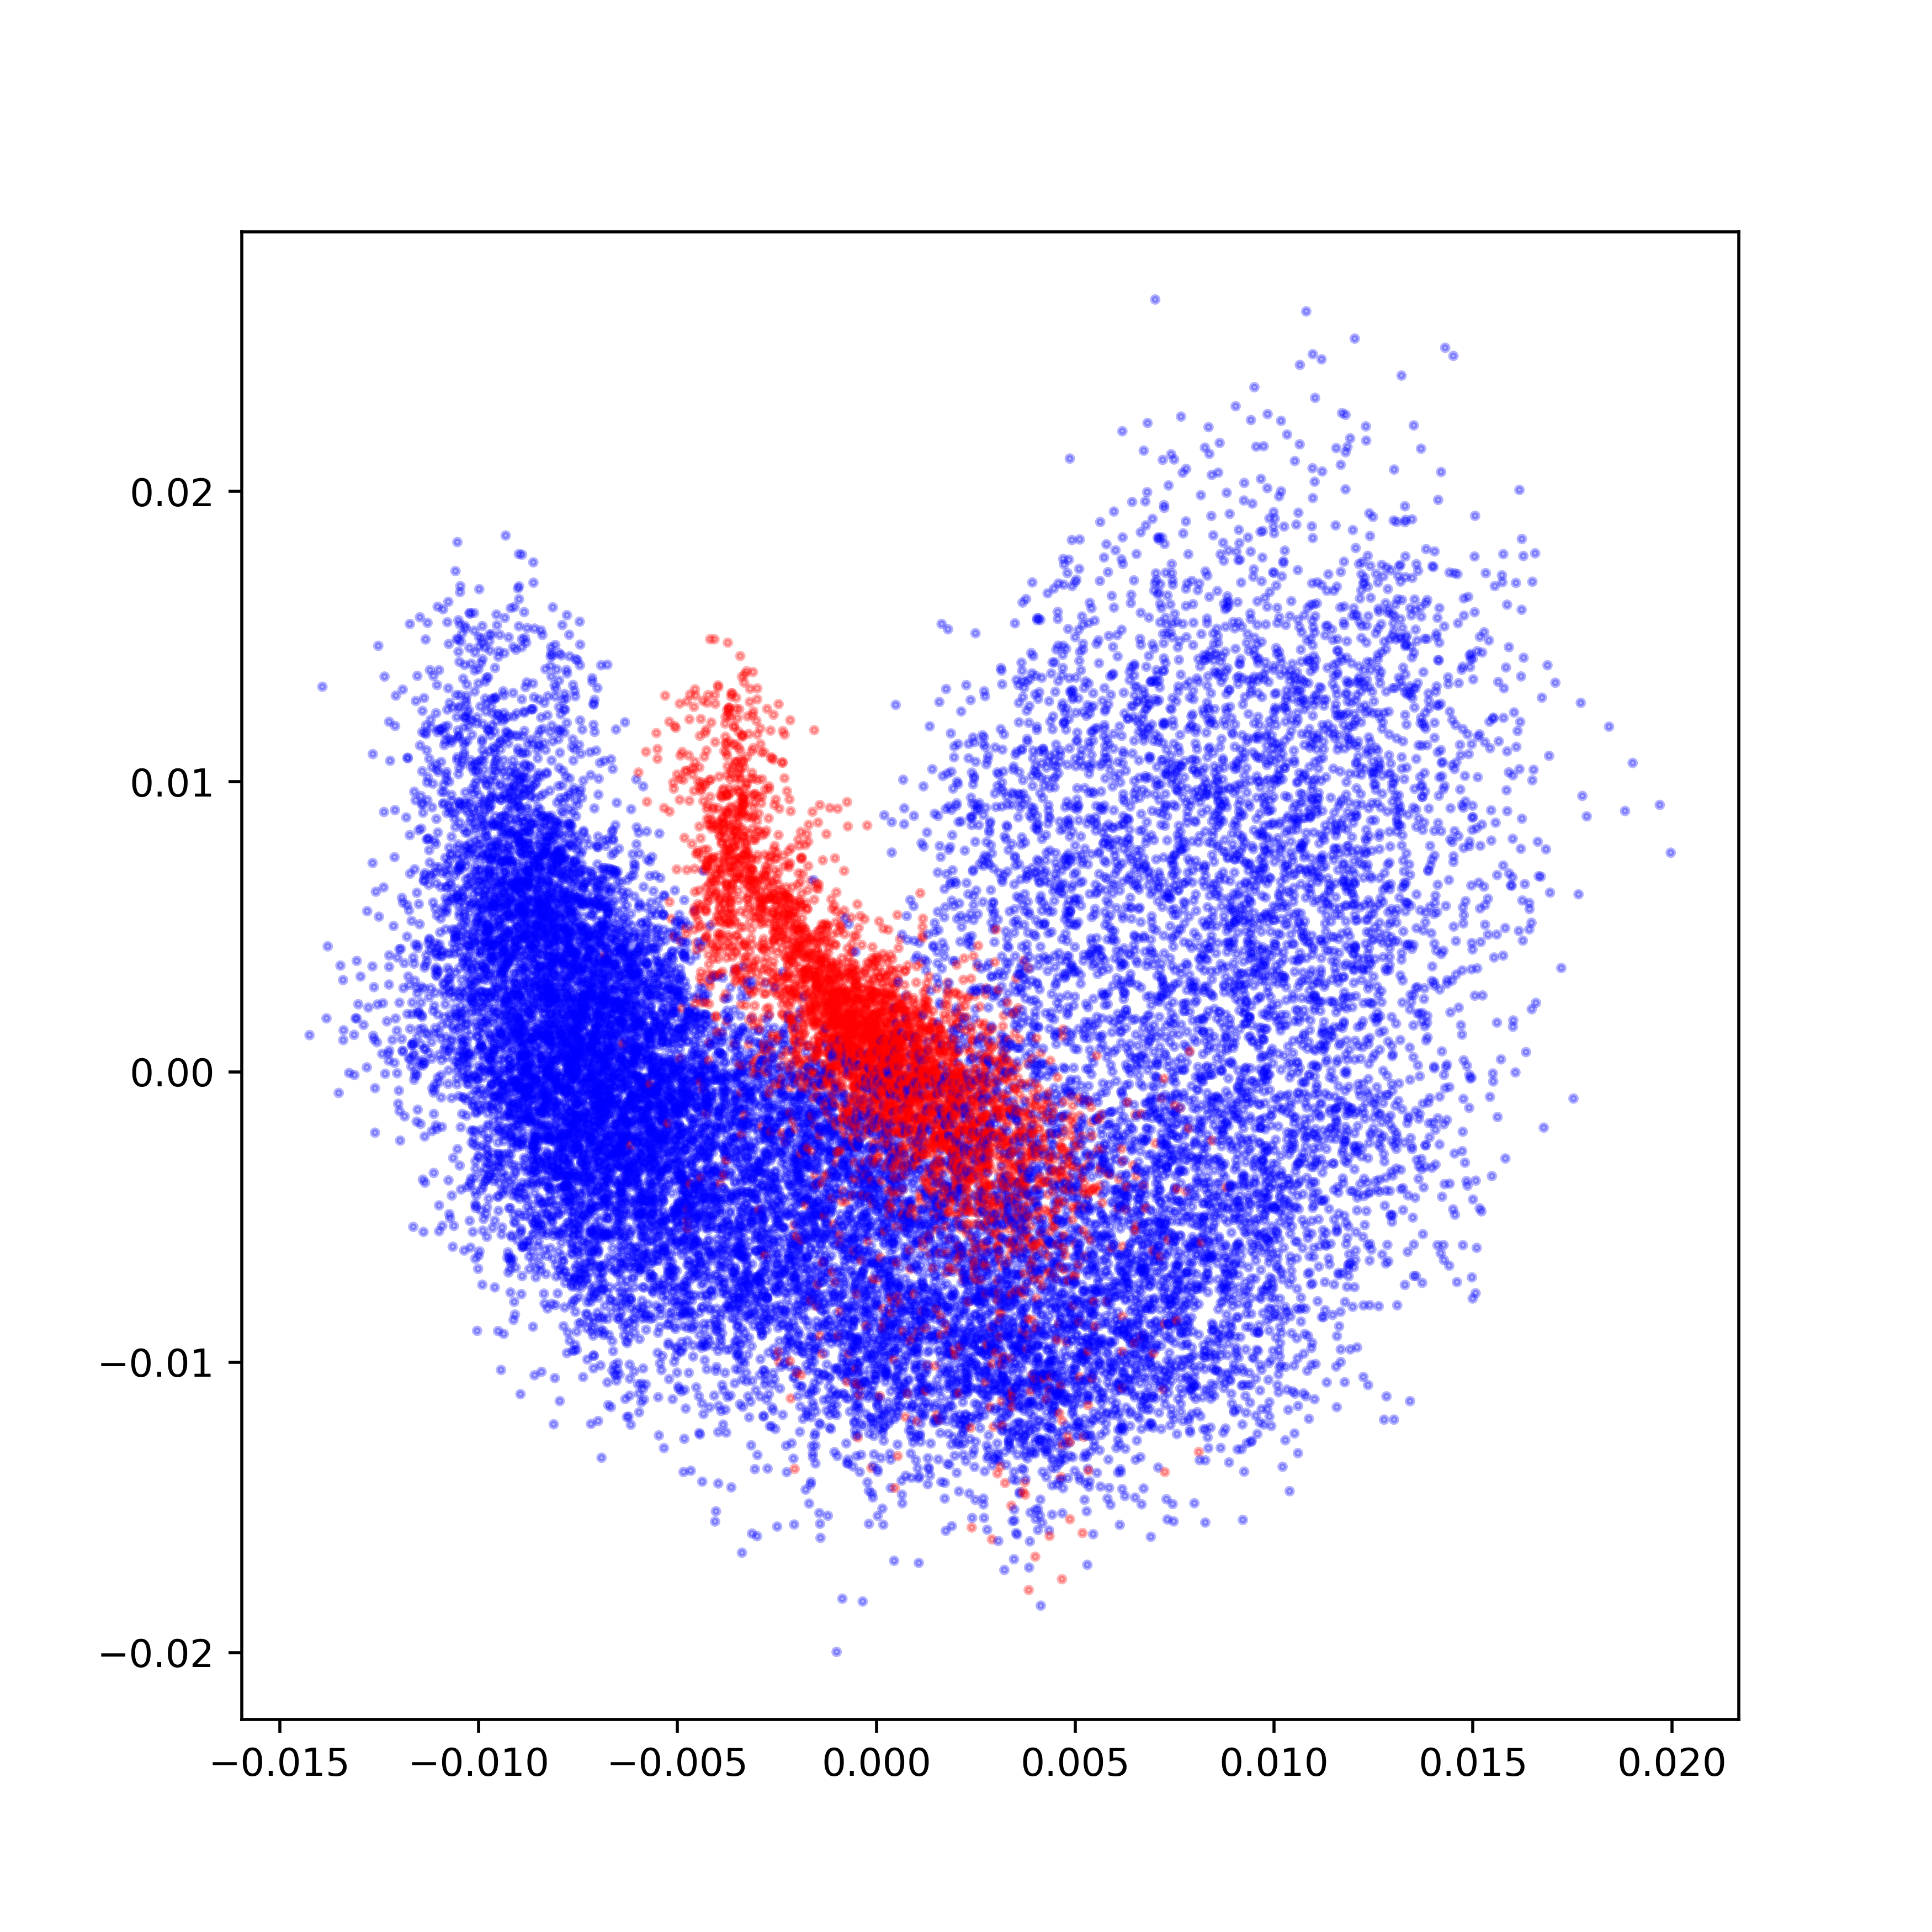
\includegraphics[width=0.9\textwidth]{Figures/Methods/ubFashion-latentspace-vis.png}
    \end{subfigure}
    \hfill
    \begin{subfigure}{0.45\textwidth}
        \centering
        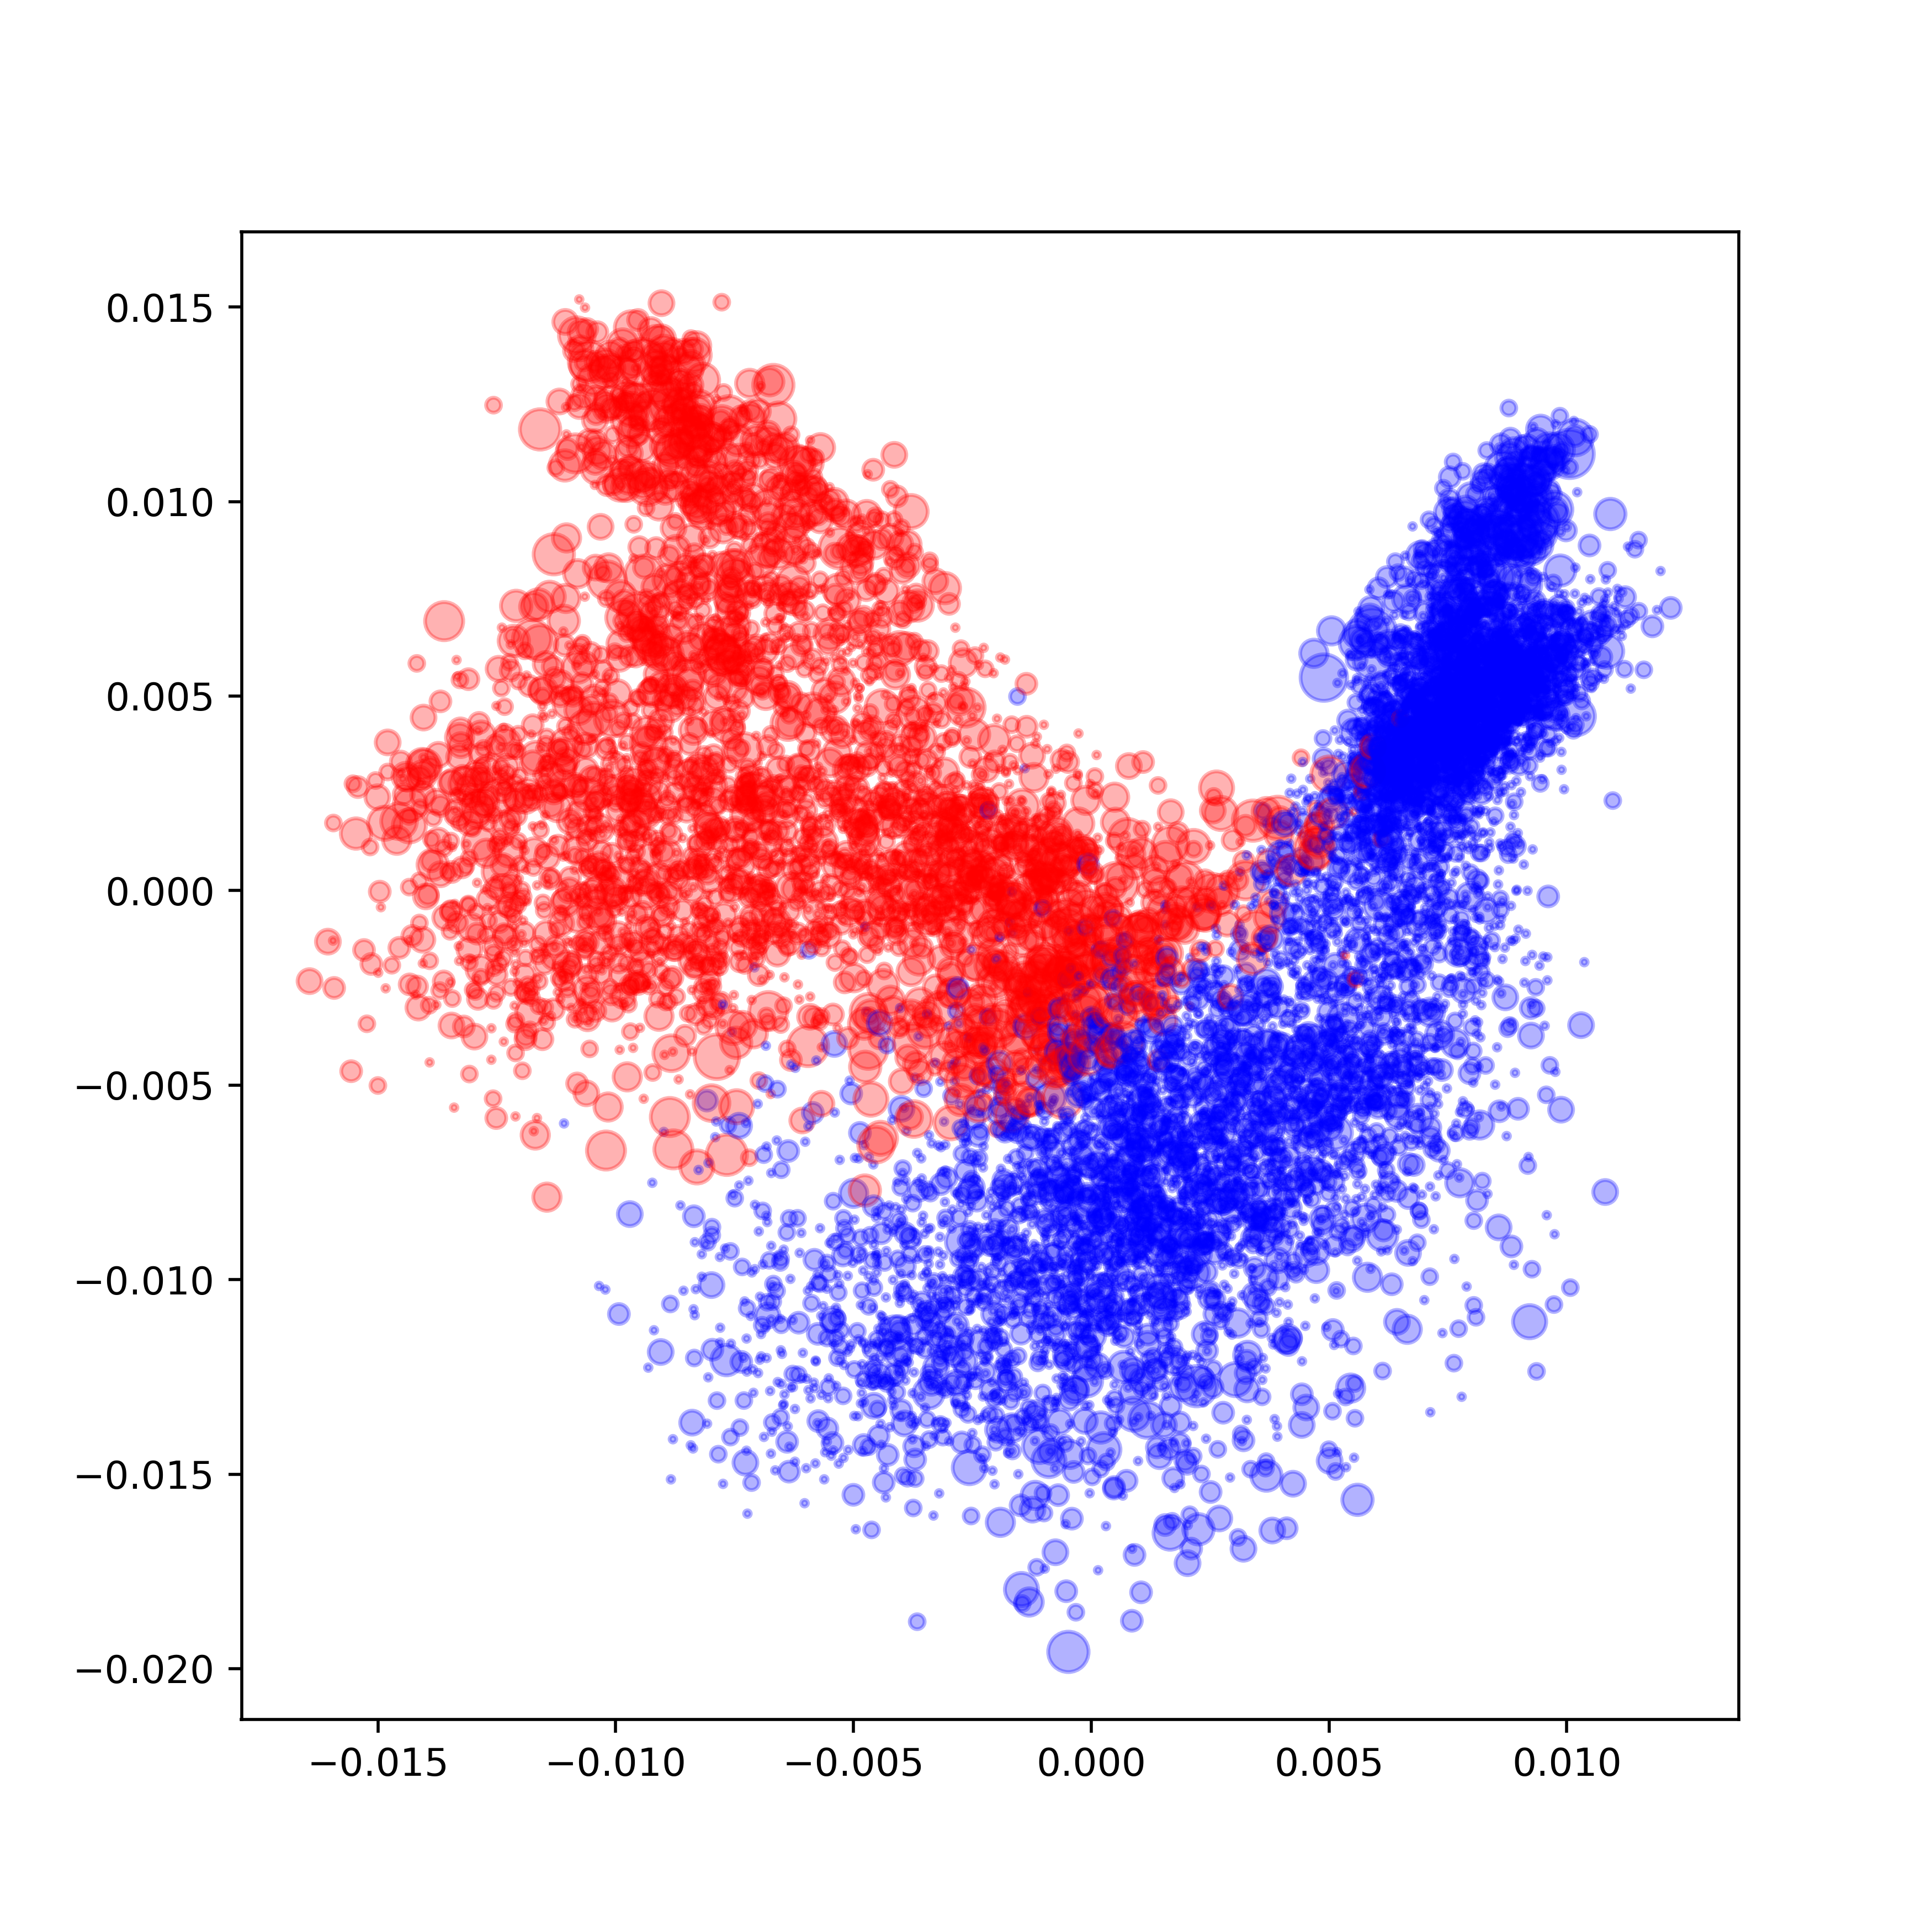
\includegraphics[width=0.9\textwidth]{Figures/Methods/RLS-ubFashion-latentspace-vis.png}
    \end{subfigure}
    \caption{Visualizations of the latent spaces of two Gen-RKMs trained on the unbalanced Fashion MNIST dataset (imbalance ratio is 0.1). Only the first two principal components in the latent spaces are displayed. The left figure is developed based on a vanilla Gen-RKM, whereas Gen-RKM in the right figure is trained with the RLS sampling (class) manner. Latent representations of minority modes are colored as red, while those of the majority classes are in blue. Note that the size of each point in the right figure indicates the frequency of being oversampled.}
    \label{fig-rls-latent-space-vis}
\end{figure}

    \item[Comparison to VAE and RLS-VAE ] A qualitative comparison is made in this section between the proposed methods and the standard VAE model. We also include the RLS sampling adapted version of VAE in this experiment to evaluate the effectiveness of RLS sampling across different model settings. The results are displayed in Table \ref{expr-comparison-vae}. Note that the same encoder and decoder architecture, along with the hyperparameter settings as outlined in Section \ref{subsec-setup-hyperparameter} is employed in VAE for a fair comparison. We observe empirically that both FID scores and KL scores are better with the Gen-RKM setting. In addition, the implementation of RLS sampling with a pre-trained classifier as feature map could significantly improve the mode coverage and capturing in both the Gen-RKM and VAE models. However, the use of RLS sampling in VAE could possibly lead to a lower FID score, indicating a poorer generation quality. 
    \begin{table}[ht]
\centering
\begin{tabular}{lcccccc}
\toprule
Model Name & Mode 1 & Mode 2 & \textbf{Mode 3} & KL Score($\downarrow$) & FID($\downarrow$) \\
\midrule
RKM & 4573(±44) & 5138(±90) & 165(±71) & 0.33(±0.02) & 61.60(±1.69) \\
RLS-RKM & 3153(±72) & 4280(±40) & \textbf{2276}(±113) & \textbf{0.03}(±0.00) & \textbf{56.65}(±1.39) \\
RLS-VAE & 3000(±78) & 4955(±198) & 1621(±262) & 0.10(±0.03) & 79.17(±2.70) \\
VAE & 4216(±101) & 5409(±154) & 176(±14) & 0.34(±0.01) & 76.39(±1.42) \\
\bottomrule
\end{tabular}
\caption{Results of comparison to VAE and RLS-VAE on the unbalanced 012-MNIST dataset with imbalance ratio 0.1. RLSs are computed by explicit feature map based on a pre-trained classifier.}
\label{expr-comparison-vae}
\end{table}

    \item[Timings of different sampling schemes ] The training times of Gen-RKM adapted with the proposed sampling schemes are reported in Table \ref{tab-sampling-training-time}. One can observe that the implementations of both RLS sampling and Iforest sampling in Gen-RKM are more computationally expensive compared to the standard training process. Among these,  RLS-RKM (shared) requires the longest training time due to the need for updating RLSs in each iteration. 
    \begin{table}[ht]
\centering
\begin{tabular}{lccc}
\toprule
{} &   Fashion &     MNIST & 012-MNIST \\
\cmidrule(lr){2-2} \cmidrule(lr){3-3} \cmidrule(lr){4-4}
Number of samples & 22200   & 32467 & 13261 \\
\midrule
Iforest RKM &  391(±18) &  721(±44) &  158(±2) \\
RKM              &   233(±5) &   326(±4) &   91(±0) \\
RLS-RKM (class)  &  418(±19) &  737(±13) &  156(±1) \\
RLS-RKM (shared) &   450(±7) &  1029(±3) &  165(±5) \\
\bottomrule
\end{tabular}
\caption{Training times in seconds (averaged over 3 runs) of different weighted sampling implementations in Gen-RKM. For the unbalanced 012-MNIST, the maximum epoch number is set to 100, while the maximum epoch number in unbalanced MNIST and Fashion MNIST is 150. The batch size is uniformly set to 328 across all cases. All experiments are conducted using a single NVIDIA GeForce RTX 3080 GPU (12GB).}
\label{tab-sampling-training-time}
\end{table}


    \item[Significance of mini-batch sampling and final step resampling ] Recall that in the RLS sampling adapted Gen-RKM, two key modifications based on weighted sampling are introduced during the training phase. Firstly, each mini-batch in every iteration is sampled with replacement according to the probability determined by the normalized RLSs. Secondly, the final computation step in Gen-RKM is performed on the full dataset, which has been resampled based on these RLSs. It is interesting to investigate how the performance of RLS-RKM becomes if we remove one of the above modifications in the algorithm. To conduct this ablation study, two simplified versions of RLS-RKM are considered as follows.
    \begin{itemize}
        \item \textbf{RLS-RKM (batch): }Only mini-batch sampling is based on RLSs, while the final computation step remains unmodified (i.e., performing KPCA on the original, unbalanced dataset). 

        \item \textbf{RLS-RKM (final): }Only the final computation step uses the resampled full dataset, while each mini-batch is uniformly sampled during the training phase, as usual.
    \end{itemize}
    The performance results of these two simplified versions of RLS-RKM are presented in Table \ref{expr-final-sample-or-mini-batch}. For RLS-RKM (batch), the performance shows almost no change compared to the vanilla RKM. This is not surprising, because the minority modes are not augmented in the latent space without the final resampling step, which inevitably makes it fail to generate more samples from the minority classes. As for RLS-RKM (final), a slight improvement on the mode coverage can be observed compared to vanilla RKM, but since the encoder and decoder parameters are not exactly trained on the resampled data, the quality of the final generation is actually worse than that of vanilla RKM. In conclusion, this ablation study demonstrates that the modifications on both mini-batch sampling and the final computation step are crucial to the effectiveness of the RLS-RKM algorithm.
    \begin{table}[ht]
\centering
\begin{tabular}{lcccccc}
\toprule
Model Name & Mode 1 & Mode 2 & \textbf{Mode 3} & KL score($\downarrow$) & FID($\downarrow$) \\
\midrule
RKM & 4623(±106) & 5185(±62) & 85(±46) & 0.36(±0.02) & 64.17(±0.28) \\
RLS-RKM & 3363(±196) & 4771(±162) & \textbf{1558}(±145) & \textbf{0.09}(±0.01) & \textbf{53.22}(±2.93) \\
RLS-RKM (batch) & 4496(±47) & 5249(±67) & 166(±17) & 0.34(±0.01) & 62.68(±2.91) \\
RLS-RKM (final) & 3759(±156) & 5111(±132) & 679(±186) & 0.21(±0.03) & 67.11(±6.06) \\
\bottomrule
\end{tabular}
\caption{Ablation study over the significance of mini-batch sampling and final step resampling in RLS-RKM. This experiment is conducted on the unbalanced 012-MNIST dataset with imbalance ratio of 0.05. RLSs are computed by an explicit feature map based on a pre-trained classifier.}
\label{expr-final-sample-or-mini-batch}
\end{table}
\end{description}


\section{Summary and discussion}
\label{sec-expr-summary}
This experiment chapter focuses on evaluating the effectiveness of different weighted sampling schemes implemented during the training of Gen-RKM on unbalanced datasets. Specifically, we conduct different experiments tailored to both supervised and unsupervised scenarios.

For the supervised setting, we assess the applicability of Gen-RKM adapted with inverse frequency sampling on the unbalanced MNIST and Fashion MNIST datasets. We then extend its use to conditional generation in the context of unbalanced data. From the results, we can conclude that
\begin{itemize}[label={--}]
\item A notable improvement in the diversity of generation can be observed when applying inverse frequency sampling. All minority modes can be successfully captured, and the distribution of generated samples becomes more uniform and balanced.
\item Unbalanced data may impact the effectiveness of conditional generation in Gen-RKM, leading to potentially blurred or incorrect results when generating samples conditioned on certain minority modes. This problem can be resolved by conditional generation based on a Gen-RKM trained with the inverse sampling manner, resulting in improved generation quality.

\item The limitation of inverse frequency sampling is quite evident. Since the sampling weights are determined by the inverse of class frequencies, it requires the knowledge of labels. Consequently, the applications of inverse frequency sampling are relatively limited in practice, as label information is often scarce in real-world scenarios.
\end{itemize}

More delicate experiments are carried out under the unsupervised setting to study the effectiveness of different RLS sampling schemes. Additionally, We also include Iforest sampling as an extension approach to basic RLS sampling. The used datasets vary from synthetic datasets to real-world image datasets. According to the results, the following findings can be concluded:
\begin{itemize}[label={--}]
    \item For the 2D synthetic dataset, we observe that RLS sampling is effective in preventing mode collapse and improving diversity in generation. However, for more complex datasets with a larger number of modes, such as the 2D grid, some minority modes may not be successfully captured.
    \item Regarding the unbalanced 012-MNIST dataset where there is only one minority mode, RLS sampling with a pre-trained classifier as the explicit feature map could significantly improve both mode coverage and generation quality under different imbalance ratios.
    \item A similar observation is made with the unbalanced MNIST and unbalanced Fashion MNIST datasets, where RLS-RKM (class) consistently outperforms other methods in terms of lower KL score and FID. However, there is a higher chance for the occurrence of mode missing due to the increasing number of minority modes in the datasets.
    \item A addition comparison to vanilla VAE and RLS-VAE is also conducted. The results indicate that using RLS sampling with VAE leads to a slightly lower FID score, suggesting a decrease in generation quality, despite great improvement in the aspect of mode coverage. Compared to Gen-RKM, the effect of RLS sampling on VAE is less pronounced.
\end{itemize}
Additionally, some drawbacks of RLS sampling can be identified from the above experiments and a series of additional studies.
\begin{itemize}[label={--}]
    \item RLS sampling is particularly dependent on the choice of feature map, which means that if the feature map fails to effectively extract information from the unbalanced data (i.e., it cannot distinguish well between minority modes and majority modes), the performance of RLS sampling could be rather poor.
    \item RLS sampling is rather computationally intensive, especially when using a shared feature map with Gen-RKM. Training could become significantly slower because the RLSs need to be recalculated in each iteration.
    \item The underlying mechanism behind RLS sampling (or possibly other weighted sampling schemes) leading to a more diverse generation in Gen-RKM is that minority modes in the latent space are also augmented via oversampling. However, this would cause the GMM to overfit, particularly on some repeated latent points, resulting in the generated samples that are very close to the true training samples. The risk of data copying in generation thus increases.
\end{itemize}

Overall, our experiments show that weighted sampling schemes like inverse frequency sampling and RLS sampling could more or less reduce the problem of mode collapse in Gen-RKM when facing unbalanced training data, leading to a more diverse and fair generation. Nevertheless, some limitations have been discovered, including the need for full label information in inverse frequency sampling, higher computational demands, the risk of data memorization, and reliance on feature maps in RLS sampling, which also suggest potential directions for future research.


% \begin{figure}[H]
%     \centering
%     \begin{subfigure}{0.45\textwidth}
%         \centering
%         \includegraphics[width=\textwidth]{Figures/Methods/rkm-fashion-gensamples-highlighted-minorities.png}
%     \end{subfigure}
%     \hfill
%     \begin{subfigure}{0.45\textwidth}
%         \centering
%         \includegraphics[width=\textwidth]{Figures/Methods/RLS-fashion-gensamples-highlighted-minorities.png}
%     \end{subfigure}
%     \caption{Generated images from unbalanced Fashion MNIST dataset by vanilla RKM (left) and RLS sampling adapted RKM (right). Feature map in RLS sampling is implemented by a pretrained classifier. Images are highlighted by a red border if classified as minority modes.}
%     \label{fig-gensamples-fashion-rls}
% \end{figure}


% \begin{figure}[H]
%     \centering
%     \begin{subfigure}{0.45\textwidth}
%         \centering
%         \includegraphics[width=\textwidth]{Figures/Methods/rkm-mnist012-gensamples-highlighted-minorities.png}
%     \end{subfigure}
%     \hfill
%     \begin{subfigure}{0.45\textwidth}
%         \centering
%         \includegraphics[width=\textwidth]{Figures/Methods/RLS-mnist012-gensamples-highlighted-minorities.png}
%     \end{subfigure}
%     \caption{Generated images from unbalanced 012-MNIST dataset by vanilla RKM (left) and RLS sampling adapted RKM (right). Feature map in RLS sampling is implemented by a pretrained classifier. Images are highlighted by a red border if classified as minority modes.}
%     \label{fig-gensamples-fashion-rls}
% \end{figure}

% \begin{figure}[H]
%     \centering
%     \begin{subfigure}{0.45\textwidth}
%         \centering
%         \includegraphics[width=\textwidth]{Figures/Methods/rkm-mnist-gensamples-highlighted-minorities.png}
%     \end{subfigure}
%     \hfill
%     \begin{subfigure}{0.45\textwidth}
%         \centering
%         \includegraphics[width=\textwidth]{Figures/Methods/RLS-mnist-gensamples-highlighted-minorities.png}
%     \end{subfigure}
%     \caption{Generated images from unbalanced MNIST dataset by vanilla RKM (left) and RLS sampling adapted RKM (right). Feature map in RLS sampling is implemented by a pretrained classifier. Images are highlighted by a red border if classified as minority modes.}
%     \label{fig-gensamples-fashion-rls}
% \end{figure}





% \begin{figure}[H]
%     \centering
%     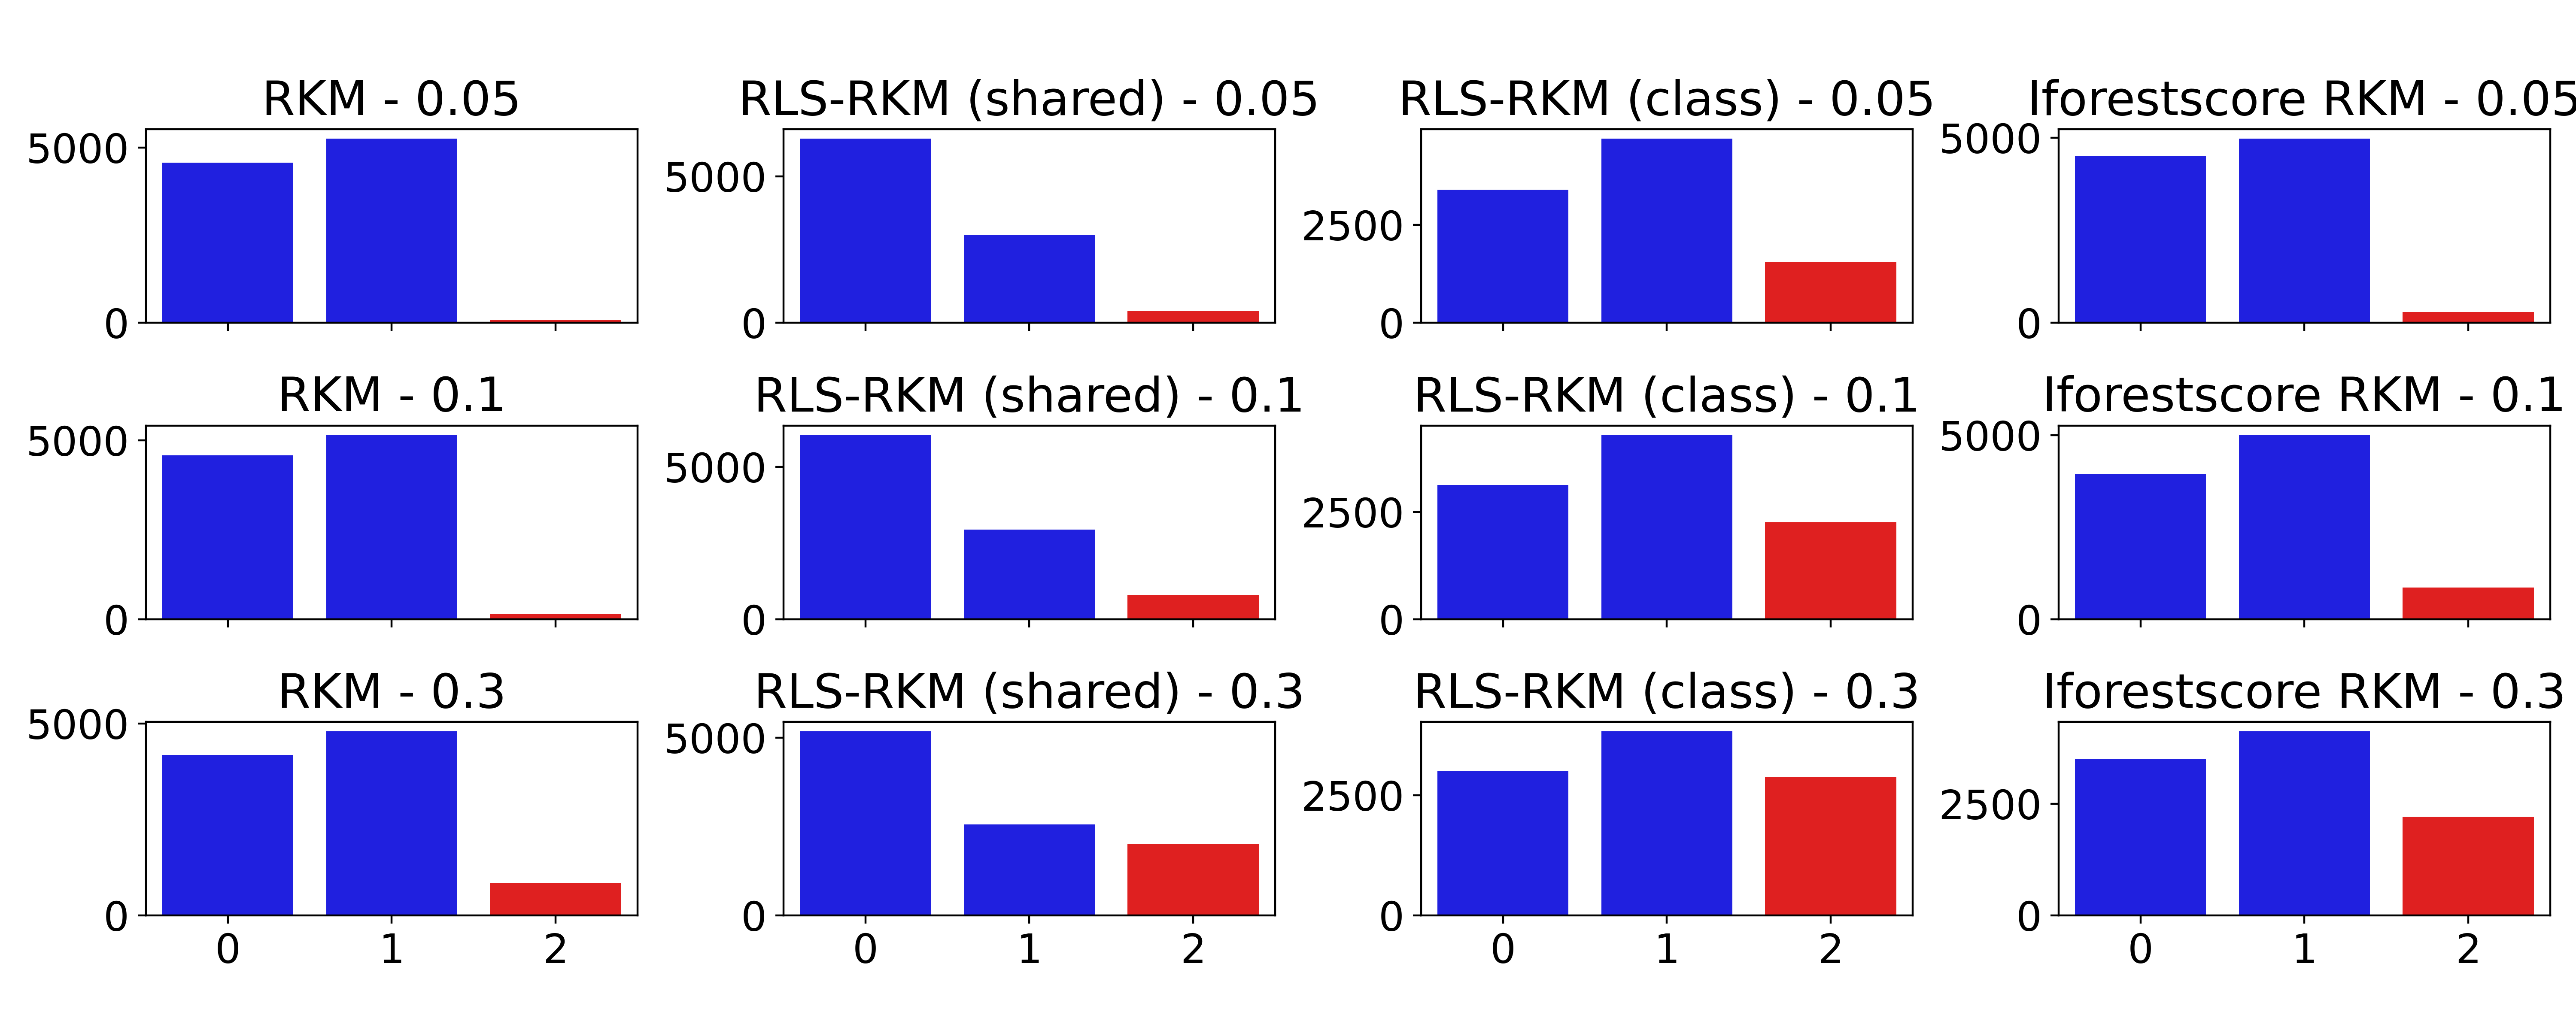
\includegraphics[width=\linewidth]{Figures/Methods/expr-mnist012-gen-dist.png}
%     \caption{Counts of generated samples per mode from different RKM models on unbalanced MNIST012 dataset.}
%     \label{fig-rls-gen-dist-ubmnist012}
% \end{figure}

% \begin{table}[ht]
    \centering
    \begin{tabular}{ccccc}
\toprule
\makecell{Imbalance \\ ratio} & Model & Minority mean & KL score ($\downarrow$) & FID ($\downarrow$) \\
\midrule
\multirow{4}{*}{0.05} & RKM & 113 (±13) & 0.49 (±0.02) & 39.19 (±1.17) \\
& RLS-RKM (shared) & 179 (±11) & 0.42 (±0.01) & 40.36 (±0.46) \\
& RLS-RKM (class) & \textbf{342} (±35) & \textbf{0.35} (±0.01) & \textbf{34.65} (±1.95) \\
& IforestRKM & 144 (±15) & 0.49 (±0.02) & 39.08 (±1.01) \\
\midrule
\multirow{4}{*}{0.10} & RKM & 185 (±11) & 0.40 (±0.01) & 38.89 (±0.18) \\
& RLS-RKM (shared) & 327 (±3) & \textbf{0.27} (±0.00) & 38.38 (±0.93) \\
& RLS-RKM (class) & \textbf{462} (±15) & \textbf{0.27} (±0.01) & \textbf{33.68} (±0.97) \\
& IforestRKM & 257 (±7) & 0.37 (±0.01) & 35.32 (±1.17) \\
\midrule
\multirow{4}{*}{0.30} & RKM & 478 (±14) & 0.15 (±0.01) & 34.09 (±1.28) \\
& RLS-RKM (shared) & 629 (±11) & \textbf{0.10} (±0.01) & 36.01 (±0.97) \\
& RLS-RKM (class) & \textbf{797} (±14) & 0.13 (±0.01) & \textbf{30.74} (±1.67) \\
& IforestRKM & 547 (±44) & 0.15 (±0.02) & 32.23 (±0.24) \\
\bottomrule
\end{tabular}
    \caption{Results of experiments on the unbalanced MNIST dataset under different imbalance ratios. Experiments are replicated over 3 runs with random initializations. Means and standard deviations (enclosed in parentheses) for each metric are reported. "Minority mean" refers to the average number of samples generated from each minority mode.
}
    \label{rls-expr-mnist}
\end{table}



% \begin{figure}[H]
%     \centering
%     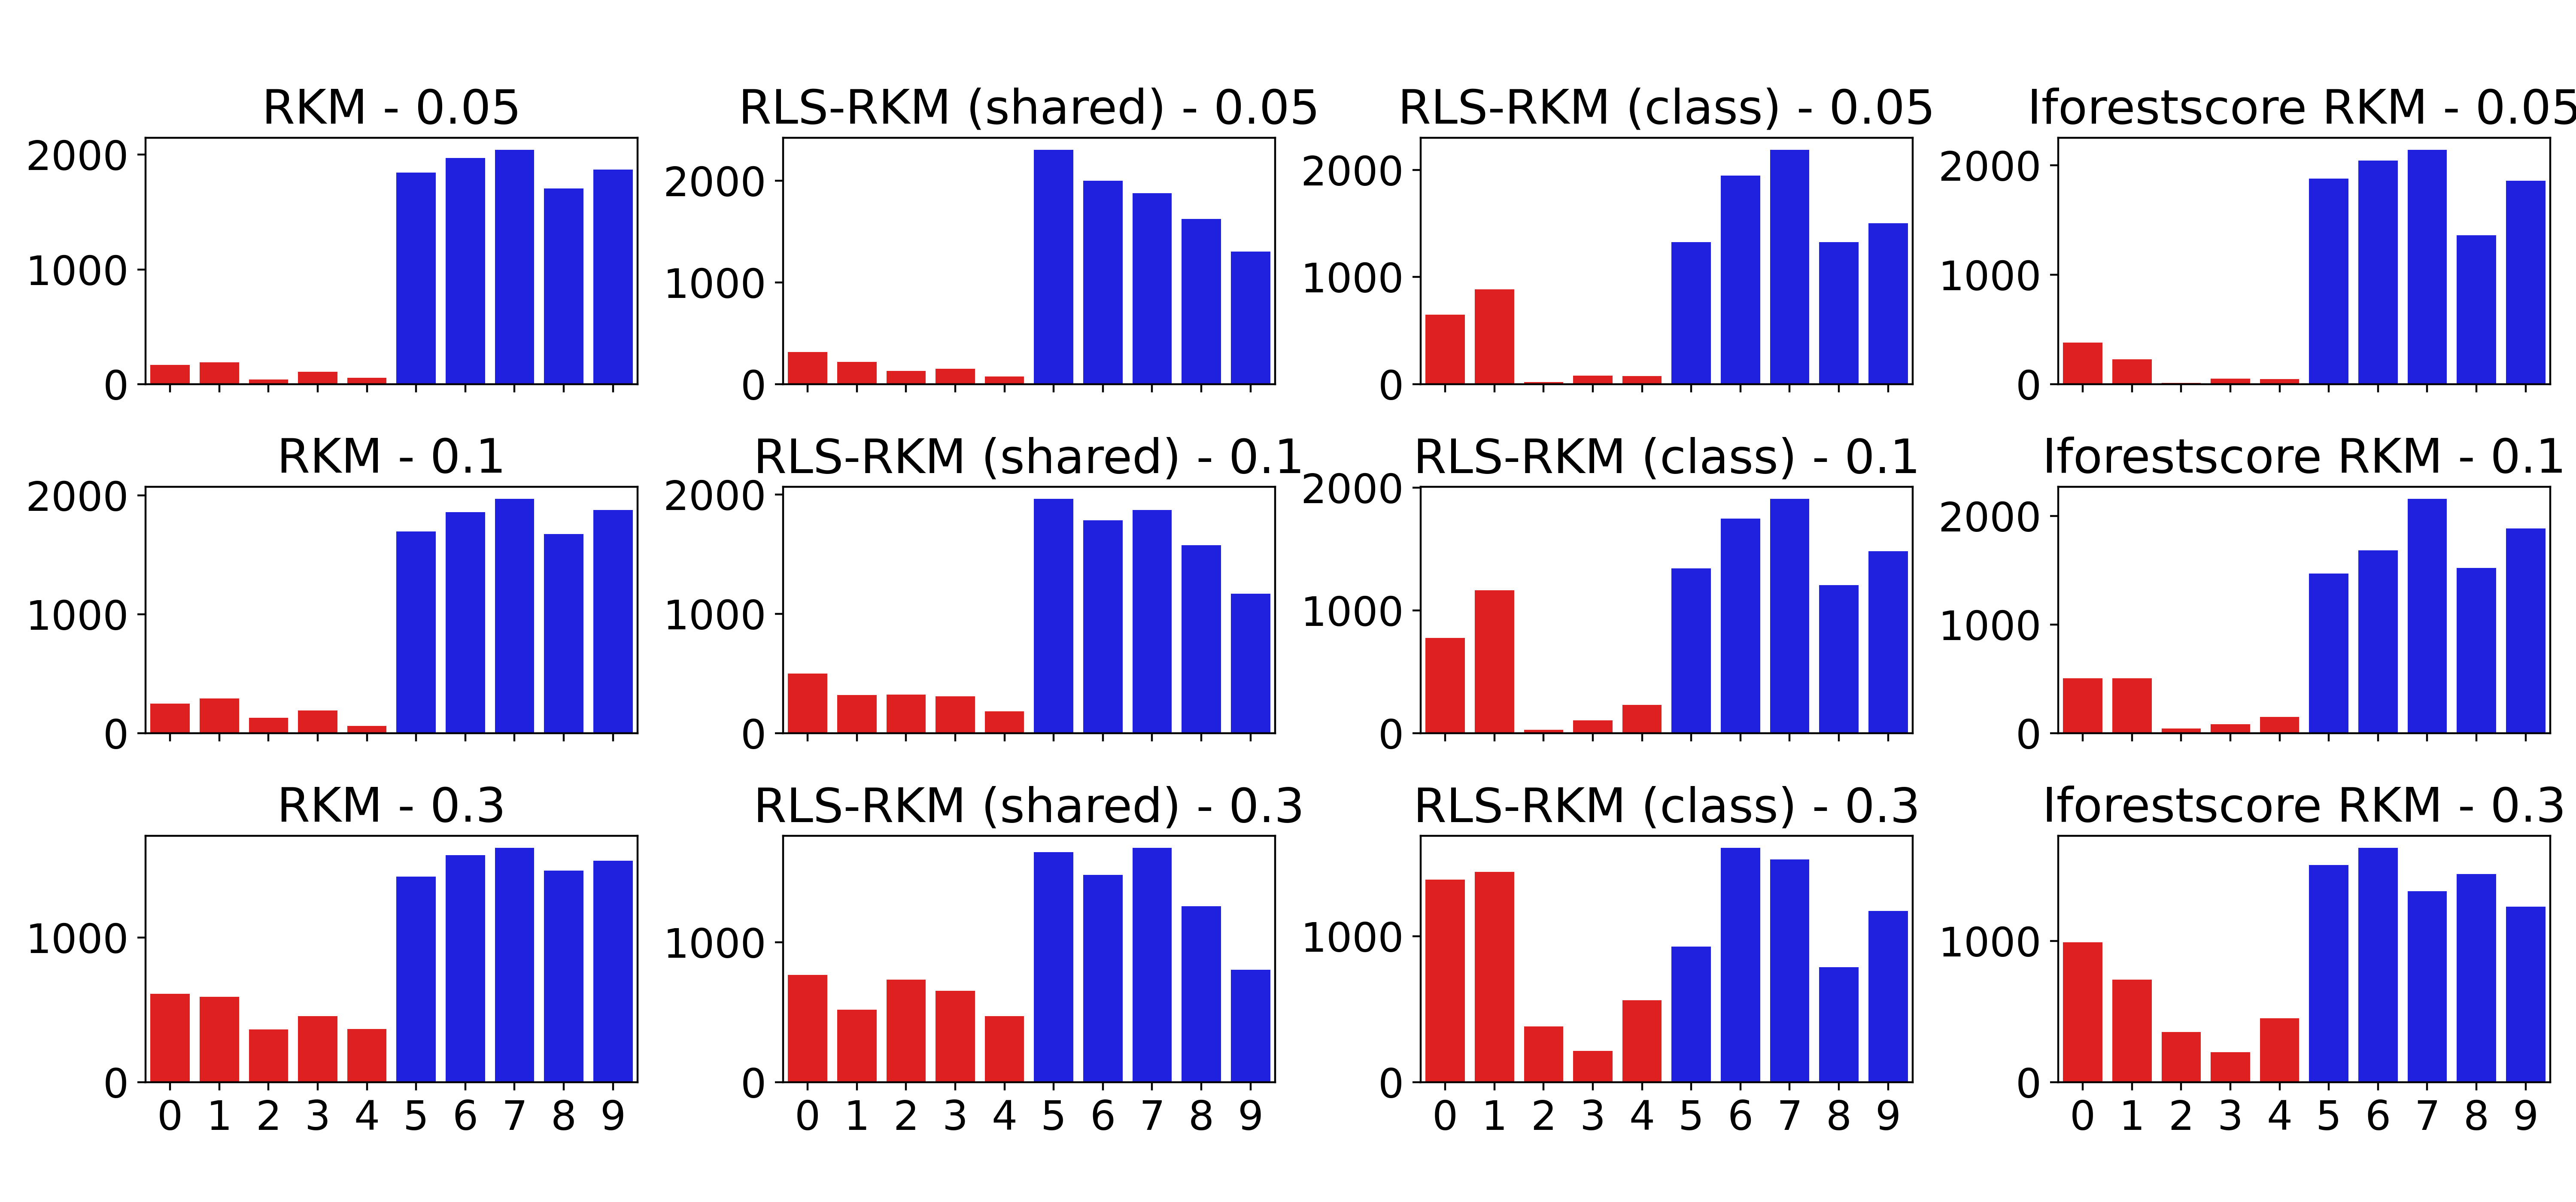
\includegraphics[width=\linewidth]{Figures/Methods/expr-rls-mnist-gen-dist.png}
%     \caption{Counts of generated samples per mode from different RKM models on unbalanced MNIST012 dataset.}
%     \label{fig-rls-gen-dist-ubmnist}
% \end{figure}
% \section{Discussion}